\documentclass[11pt,twoside]{book}
\usepackage{times,mathptm,multirow,fancyvrb,color}
\usepackage{picins}

%\usepackage{wrapfig}
\usepackage[pdftex]{graphicx}
\usepackage{hyperref}
\pdfcompresslevel=9
\DeclareGraphicsExtensions{.jpg,.pdf,.png}
\usepackage{setspace,moreverb}

%\usepackage{eso-pic}
\usepackage{color}

%\makeatletter
%   \AddToShipoutPicture{%
%     \setlength{\@tempdimb}{.5\paperwidth}%
%     \setlength{\@tempdimc}{.5\paperheight}%
%     \setlength{\unitlength}{1pt}%
%     \put(\strip@pt\@tempdimb,\strip@pt\@tempdimc){%

%\makebox(0,0){\rotatebox{45}{\textcolor[gray]{0.75}{\fontsize{8cm}{8cm}\selectfont{DRAFT}}}}
%    }
% }
%\makeatother

\pagestyle{empty}

\setlength{\textwidth}{6.5in}
\setlength{\oddsidemargin}{0.00in}
\setlength{\evensidemargin}{0.0in}



\setlength{\textheight}{9.0in}
\setlength{\topmargin}{0.00in}
\setlength{\parindent}{0.2in}

\setlength{\headheight}{0.00in}
\setlength{\headsep}{0.0in}
\setlength{\paperheight}{11.0in}
\setlength{\paperwidth}{8.5in}
%
% new commands for this paper
%
\newcommand{\bverb}{
\begin{Verbatim}[frame=single,rulecolor=\color{blue},
framerule=3pt,framesep=1pc,fillcolor=\color{yellow}]
}
\newcommand{\everb}{
\end{Verbatim}
}
\newcommand{\degC}{$^\circ$C}
\newcommand{\figoptions}{P}
\newcommand{\hhref}[1]{\href{#1}{{\tt #1}
}}
\newcommand{\figheight}{1.5in}
\newcommand{\infigheight}{0.75in}
\newcommand{\figheightA}{2.5in}
\newcommand{\figheightAbar}{2.2in}
\newcommand{\figheightC}{2.5in}
\newcommand{\figwidth}{3.333333in}
\newcommand{\figwidthb}{2.0in}
\newcommand{\FDS}{{FDS}}
\newcommand{\fds}{{FDS}}
\newcommand{\Smokeview}{{Smokeview}}
\newcommand{\smokeview}{{Smokeview}}
\newcommand{\parma}{.75}
\newcommand{\parmb}{.5}
\newcommand{\parmc}{0.25}
\newcommand{\bold}[1]{{\bf #1}}
\newcommand{\etc}{{\em etc}}
\newcommand{\ie}{{\em i.e.}}
\newcommand{\eg}{{\em e.g.}}
\newcommand{\via}{{via\ }}
\newcommand{\dialoguenmenu}{\fbox{\tt Diaglog} }
\newcommand{\optionmenu}{\fbox{\tt Option} }
\newcommand{\loadmenu}{\fbox{\tt Load/Unload} }
\newcommand{\tourmenu}{\fbox{\tt Tour} }
\newcommand{\helpmenu}{\fbox{\tt Help} }
\newcommand{\setbounds}{\fbox{\tt Set Bounds} }
\newcommand{\showmenu}{\fbox{\tt Show/Hide} }
\newcommand{\frameit}[1]{\fbox{\tt #1}}
\newcommand{\blist}{
\begin{list}
{}{
\setlength{\leftmargin}{\parma in}
\setlength{\labelwidth}{\parmb in}
\setlength{\labelsep}{\parmc in}
\setlength{\listparindent}{0.3in}
\setlength{\topsep}{.3in}
\setlength{\parsep}{.0in}
}}
\newcommand{\elist}{\end{list}}
\newcommand{\hitem}[1]{\item[{\bf #1} \hfill]}

\bibliographystyle{unsrt}
%\doublespace
\begin{document}
\newcommand{\ttitle}{User's Guide for Smokeview Version 4 \\
- A Tool for Visualizing Fire Dynamics Simulation Data}
%
% ----------------------  first cover/title page --------------------------
%
\begin{minipage}[t][9in][s]{6.5in}

\huge
\flushright{NIST Special Publication 1017-1}


\vspace{1in}

\Huge
\flushright{User's Guide for Smokeview Version 5 \\
- A Tool for Visualizing Fire Dynamics Simulation Data}
\flushright{(Draft: May 28, 2007)}

\vspace{.5in}
\normalsize
\flushright{Glenn P. Forney}

\vfill


\includegraphics[width=\textwidth]{figures/nistlogo_1line}

\end{minipage}

\newpage

%
% ----------------------  second cover/title page --------------------------
%
\begin{minipage}[t][9in][s]{6.5in}

\huge
\flushright{NIST Special Publication 1017-1}

\vspace{1.in}

\Huge
\flushright{User's Guide for Smokeview Version 5 \\
- A Tool for Visualizing Fire Dynamics Simulation Data}

\vspace{.5in}

\normalsize
\flushright{Glenn P. Forney\\
%\includegraphics[width=1in]{FIGURES/bfrl}  \\
{\em Fire Research Division} \\
{\em Building and Fire Research Laboratory}  \\
}

\vspace{.25in}

\flushright{June 2007}

\vfill

\flushright{
\includegraphics[width=1in]{figures/doc} }

\small
\flushright{U.S. Department of Commerce \\
{\em Carlos M. Gutierrez, Secretary} \\
\hspace{1in} \\
Technology Administration \\
{\em Robert Cresanti, Under Secretary for Technology}  \\
\hspace{1in} \\
National Institute of Standards and Technology \\
{\em William A. Jeffrey, Director} }


\end{minipage}


\date{}
%\pubnumber{xxxx}
\title{\ttitle}
\author{Glenn P. Forney}

%\pubdate{February 2001}
%\makecover{1}

\setlength{\parindent}{0.25in}

\newpage

\begin{minipage}[t][9in][s]{6.5in}

\flushright{Certain commercial entities, equipment, or materials may be identified in this \\
document in order to describe an experimental procedure or concept adequately. Such \\
identification is not intended to imply recommendation or endorsement by the \\
National Institute of Standards and Technology, nor is it intended to imply that the \\
entities, materials, or equipment are necessarily the best available for the purpose.
}

\vspace{3in}

\large
\flushright{\bf National Institute of Standards and Technology Special Publication 1017-1 \\
Natl.~Inst.~Stand.~Technol.~Spec.~Publ.~1017-1, 116 pages (June 2007) \\
CODEN: NSPUE2 }

\vfill

\flushright{U.S. GOVERNMENT PRINTING OFFICE \\
WASHINGTON: 2004 \\
\rule{3.5in}{0.01in} \\
For sale by the Superintendent of Documents, U.S. Government Printing Office \\
Internet: bookstore.gpo.gov -- Phone: (202) 512-1800 -- Fax: (202) 512-2250 \\
Mail: Stop SSOP, Washington, DC 20402-0001 }

\end{minipage}


\frontmatter

\pagestyle{plain}

%---------------------------------------------------------------------------------
%------------------------ Preface ------------------------------------------------
%---------------------------------------------------------------------------------

\chapter{Preface}
\Smokeview\ is a software tool designed to visualize numerical
calculations generated by the NIST Fire Dynamics Simulator (\fds),
a computational fluid dynamics (CFD) model of fire-driven fluid
flow. For details on setting up and running FDS cases read the FDS
User's guide\cite{FDS_Users_Guide_5}.  These two tools are
typically used together to respectively simulate and visualize the
flow of smoke induced by a fire. Smokeview visualizes the smoke
using traditional scientific methods such as displaying tracer
particle flow, 2D or 3D shaded contours of gas flow data such as
temperature and flow vectors showing flow direction and magnitude.
Smokeview also visualizes smoke realistically so that one can
{\em experience}\ the fire. This is done by displaying a series of
partially transparent planes where the transparencies in each
plane (at each grid node) are determined from soot densities
computed by FDS.  \Smokeview\ also visualizes static data at
particular times again using 2D or 3D contours of data such as
temperature and flow vectors showing flow direction and magnitude.

Windows PC versions of \Smokeview\ and \fds\ and associated
documentation may be downloaded from the web site {\bf
\hhref{http://fire.nist.gov/smokeview}} at no cost.
Versions for Linux and Mac/OSX may also be downloaded from
the same location.

%---------------------------------------------------------------------------------
%------------------------ Disclaimer ---------------------------------------------
%---------------------------------------------------------------------------------

\chapter{Disclaimer}

The US Department of Commerce makes no warranty,
expressed or implied, to users of Smokeview, and accepts no
responsibility for its use. Users of Smokeview assume sole
responsibility under Federal law for determining the
appropriateness of its use in any particular application; for any
conclusions drawn from the results of its use; and for any actions
taken or not taken as a result of analysis performed using this
tools.

Smokeview and the companion program FDS is intended for use only
by those competent in the fields of fluid dynamics,
thermodynamics, combustion, and heat transfer, and is intended
only to supplement the informed judgment of the qualified user.
These software packages may or may not have predictive capability
when applied to a specific set of factual circumstances. Lack of
accurate predictions could lead to erroneous conclusions with
regard to fire safety. All results should be evaluated by an
informed user.

Throughout this document, the mention of computer hardware or
commercial software does not constitute endorsement by NIST,
nor does
it indicate that the products are necessarily those
best suited for the
intended purpose.

%---------------------------------------------------------------------------------
%------------------------ Acknowledgements ---------------------------------------
%---------------------------------------------------------------------------------

\chapter*{Acknowledgements}
A number of people have made significant contributions to the
development of Smokeview. In trying to acknowledge those that have
contributed, we are inevitably going to miss a few people - let us
know and we will include those missed in the next version of this
guide.

The original version of Smokeview was inspired by Frames, a
visualization program written by James Sims for the Silicon
Graphics workstation.  This software was based on visualization
software written by Stuart Cramer for an Evans and Sutherland
computer. Frames used tracer particles to visualize smoke flow
computed by a pre-cursor to FDS. Judy Devaney made the NIST
multi-screen eight foot Rave facility available allowing a stereo
version of Smokeview to be built that can display scenes in
3D.  Both Steve Satterfield and Tere Griffin on many occasions
helped me demonstrate Smokeview cases on the Rave inspiring many
people to the possibility of using Smokeview as a {\em virtual
reality-like}\ fire fighter training facility.

Many conversations with Nelson Bryner, Dave Evans, Anthony Hamins
and Doug Walton were most helpful in determining how Smokeview
could be adapted for use in fire fighter training applications.

Smokeview would not be possible without the use of a number of
software libraries developed by others.  Mark Kilgard while at
Silicon Graphics developed GLUT, the basic tool kit for
interfacing OpenGL with the underlying operating system on
multiple computer platforms. Paul Rademacher while a graduate
student at the University of North Carolina developed GLUI, the
software library for implementing the user friendly dialog boxes.

Significant contributions have been made by those that have used
Smokeview to visualize complex cases; cases that are used to
perform both applied and basic research.  The resulting feedback
has improved Smokeview as a result of their interaction with me,
pushing the envelope and not accepting the status quo.

For applied research, Daniel Madrzykowski, Doug Walton and Robert
Vettori of NIST have used Smokeview to analyze fire incidents.
Steve Kerber has used Smokeview to visualize flows resulting from
PPV fans. David Stroup has used Smokeview to analyze cases for use
in fire fighter training scenarios.  Conversations with Doug
Walton have been particularly helpful in identifying needed
features and clarifying how best to make their implementation user
friendly.  David Evans, William (Ruddy) Mell and Ronald Rehm used
Smokeview to visualize {\em urban-wildland interface}\ fires.   For
basic research, Greg Linteris has used Smokeview to visualize fire
simulations involving the cone calorimeter. Anthony Hamins has
used Smokeview to visualize the structure of CH4/air flames
undergoing the transition from normal to microgravity conditions
and fire suppression in a compartment. Jiann Yang has used
Smokeview to visualize smoke or particle number density and
saturation ratio of condensable vapor.

This user's guide has improved through the many constructive
comments of the reviewers Anthony Hamins, Doug Walton, Ronald
Rehm, and David Sheppard. Chuck Bouldin helped port Smokeview to
the Macintosh.

Many people have sent in multiple comments and feedback by email,
in particular Adrian Brown, Scot Deal, Charlie Fleischmann, Jason
Floyd, Simo Hostikka, Bryan Klein, Davy Leroy, Dave McGill, Brian
McLaughlin, Derek Nolan, Steven Olenick, Stephen Priddy, Boris
Stock, Jason Sutula, Javier Trelles, and Christopher Wood.

Feedback is encouraged and may be sent to glenn.forney@nist.gov .

\tableofcontents
\listoffigures
\listoftables

\mainmatter

\pagenumbering{arabic}

%
% .............. new section ..............................
%
%\pagestyle{fancy}
%\newcounter{picno}
%\setcounter{picno}{24}
%\newcounter{picnoe}
%\setcounter{picnoe}{24}
%\fancyhead{} \fancyfoot[RO] {
% \setlength{\unitlength}{1mm}
% %\stepcounter{picno}
% \addtocounter{picno}{-1}
% \begin{picture}(0,0)
%   \put(-15,0){
%     \epsfig{height=1.125in,figure=figures/movies/tankfarm_\number\value{picno}.eps}
%   }
% \end{picture}
%}
%
%\fancyfoot[LE]
%{
%  \setlength{\unitlength}{1mm}
%  %\stepcounter{picnoe}{-1}
%  \addtocounter{picnoe}{-1}
%  \begin{picture}(0,0)
%    \put(-15,0){
%      \epsfig{height=1.25in,figure=figures/movies/townhouse3_\number\value{picnoe}.eps}
%    }
%  \end{picture}
%}
%\renewcommand{\headrulewidth}{0.0pt}
%\renewcommand{\footrulewidth}{0.0pt}
%\renewcommand{\footskip}{1.5in}

%---------------------------------------------------------------------------------
%------------------------ Introduction -------------------------------------------
%---------------------------------------------------------------------------------

\chapter{Introduction}
\section{Overview}
\Smokeview\ is a software tool designed to visualize numerical
predictions generated by the NIST Fire Dynamics Simulator (\fds),
a computational fluid dynamics (CFD) model of fire-driven fluid
flow\cite{FDS_Tech_Guide_5}. This report documents version 5 of
\smokeview\ updating material found in Ref.
\cite{Smokeview_Users_Guide_4}. For details on setting up and
running FDS cases read the FDS User's
guide\cite{FDS_Users_Guide_5}.

\FDS\ and \smokeview\ are used to model and visualize fire
phenomena. However, FDS and Smokeview are not limited to fire
simulation. For example, one may use FDS and \smokeview\ to model
other applications such as contaminant flow in a building.
\Smokeview\ performs this visualization by displaying time
dependent tracer particle flow, animated contour slices of
computed gas variables and surface data. \Smokeview\ also presents
contours and vector plots of static data anywhere within a
simulation scene at a fixed time. Several examples using these
techniques to investigate fire incidents are documented in Refs.
\cite{CHERRYROAD,IOWA,HOUSTON,WTC}.

Normally \smokeview\ is used in a post-processing step to
visualize \fds\ data after a calculation has been completed.
\Smokeview\  may also be used during a calculation to monitor a
simulation's progress and before a calculation to setup \fds\
input files more quickly, one can then use \smokeview\ to edit or
create blockages by specifying the size, location and/or material
properties.

Figure \ref{figfdsoverview} gives an overview of how data files
used by FDS,  Smokeview and Smokezip are related. A typical
procedure for using \fds\ and \smokeview\ is to:
\begin{enumerate}

\item Set up an \fds\ input file.

\item Run \fds.  \fds\ then creates one or more output files used
by Smokeview to visualize the case.

\item Run \smokeview\ to analyze the output files generated by
step 2. by either double-clicking the file named {\tt
casename.smv} with the mouse (on the PC) or by typing {\tt
smokeview casename} at a command line. \Smokeview\ may also be
used to create new blockages and modify existing ones. The
blockage changes are saved in a new \fds\ input data file.
\end{enumerate}

\noindent This publication documents step 3. Steps 1 and 2 are documented in
the FDS User's Guide \cite{FDS_Users_Guide_5}.

\begin{figure}[\figoptions]
\centerline{
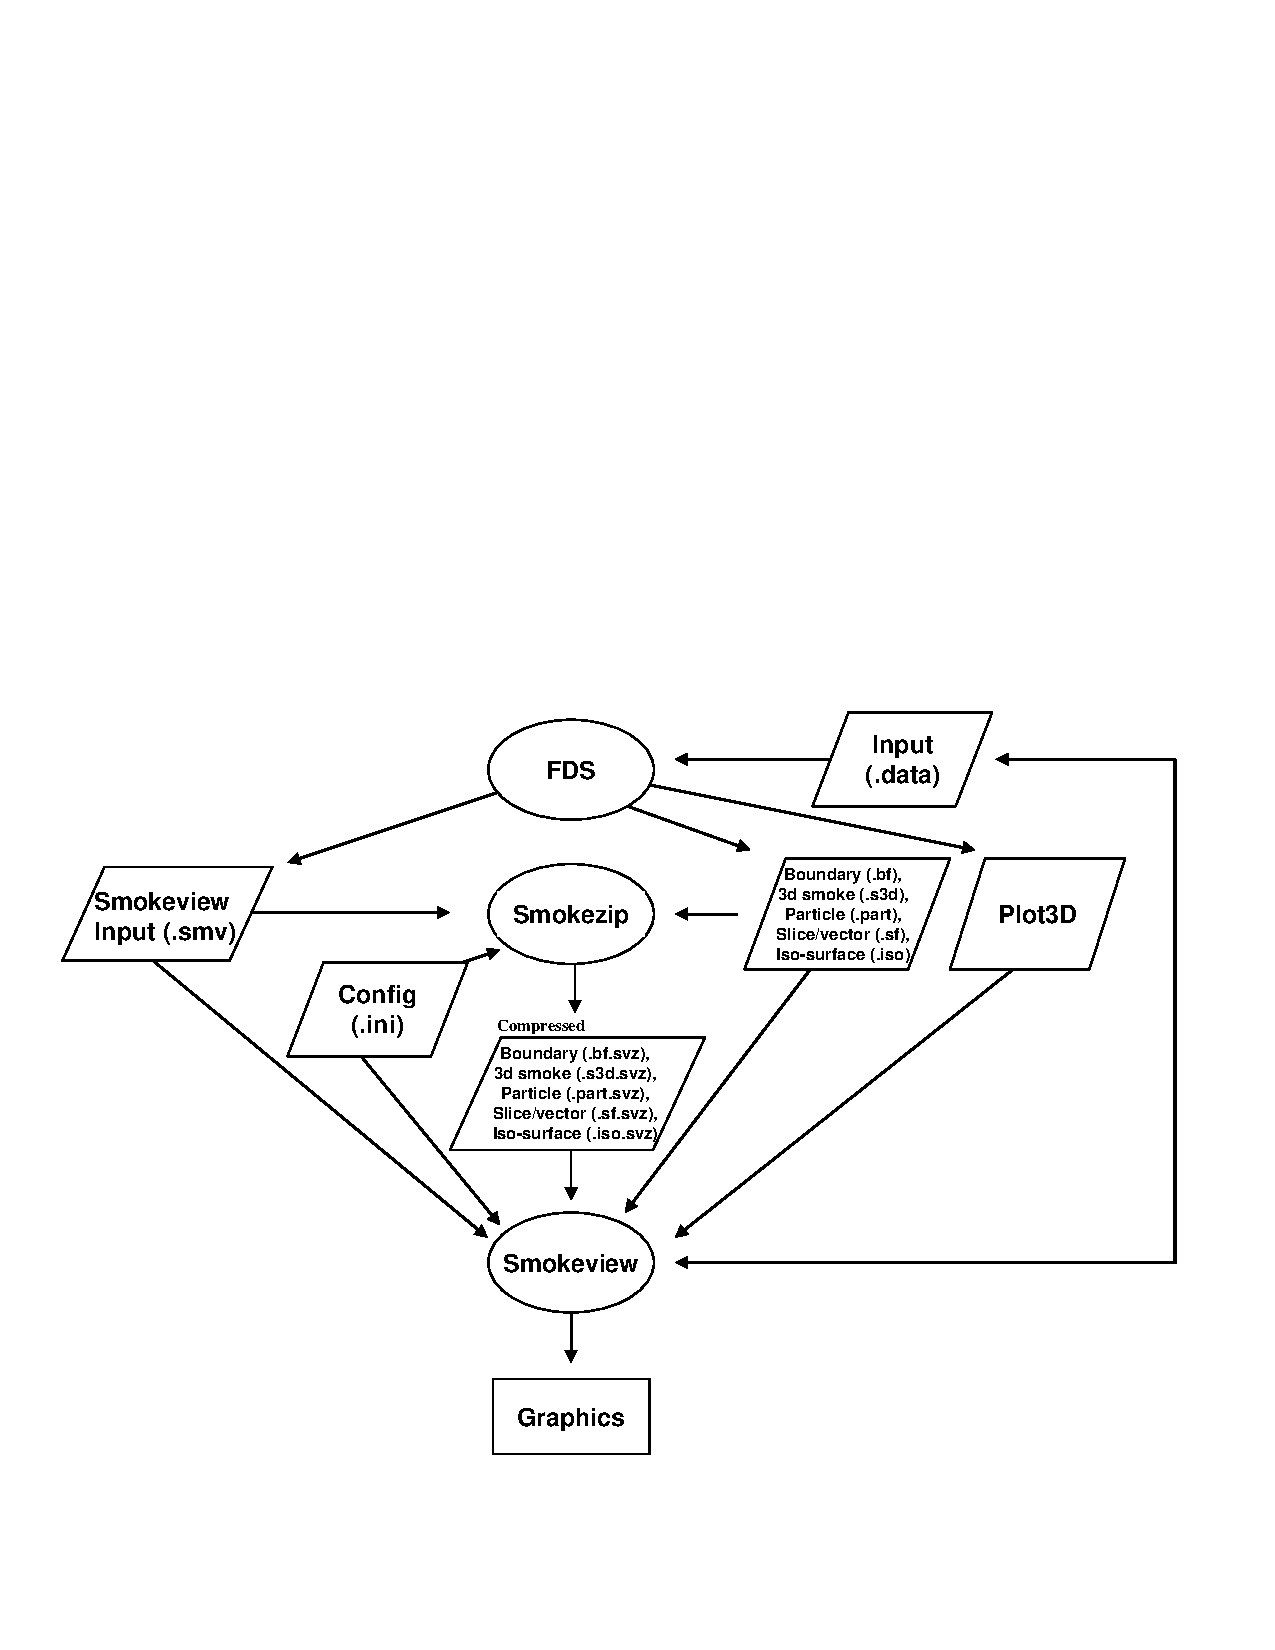
\includegraphics[width=5.0in]{figures/fds_overview}}
 \caption[FDS file overview]{Diagram illustrating files used and created by the NIST Fire Dynamics
 Simulator (FDS), Smokezip and Smokeview.}
\label{figfdsoverview}%
\end{figure}

Menus in Smokeview are activated by clicking the right mouse
button anywhere in the Smokeview window.  Data files may be
visualized by selecting the desired \loadmenu\ menu option. Other
menu options are discussed in Appendix \ref{sectionmenu}. Many
menu commands have equivalent keyboard shortcuts. These shortcuts
are listed in \smokeview's \helpmenu\ menu and are described in
Appendix \ref{sectionkeyboard}. Visualization features not
controllable through the menus may be customized by using the
\smokeview\ preference file, {\tt smokeview.ini}, discussed in
Appendix \ref{appendixini}.

\Smokeview\ is written in C and Fortran 90 and consists of about
70,000 lines of code. The C portion of Smokeview visualizes the
data while the Fortran 90 portion reads in the data generated by
FDS (also written in Fortran 90). \smokeview\ uses the 3D graphics
library OpenGL\cite{OpenGLRed3} and the Graphics Library Utility
Toolkit (GLUT)\cite{OpenGLGlut}. \Smokeview\ uses the GLUT
software library so that most of the development effort can be
spent implementing the visualizations rather than creating an
elaborate user interface.  \Smokeview\ uses a number of auxiliary
libraries to implement image capture (GD\cite{BOUTELL,GDLIB},
PNG\cite{PNGLIB}, JPEG\cite{JPEGLIB}), image and general file
compression (ZLIB\cite{ZLIB}) and dialog creation
(GLUI\cite{GLUILIB}). Each of these libraries is portable running
under UNIX, LINUX and Windows 9x/2000/XP allowing Smokeview to run
on these platforms as well.

\section{Features}

Smokeview is a program designed to visualize numerical
calculations generated by the Fire Dynamics Simulator.
Smokeview visualizes both dynamic and static data.  Dynamic
data is visualized by animating particle flow (showing
location and {\em values}\ of tracer particles), 2D contour
slices (both within the domain and on solid surfaces) and
3D level surfaces.  2D contour slices can also be drawn
with colored vectors that use velocity data to show flow
direction, speed and value. Static data is visualized
similarly by drawing 2D contours, vector plots and 3D level
surfaces. Smokeview features in more detail include:

\begin{description}
\item[3D Smoke] Smoke, fire and sprinkler spray are displayed
realistically using a series of partially transparent planes.  The
smoke transparencies are determined by using smoke densities
computed by FDS.  The fire and sprinkler spray transparencies are
determined by using a heuristic based on heat release rate and
water density data, again computed by FDS. Various settings for
the 3d smoke option may be set using the new {\em 3D Smoke}\ dialog
box found in the \frameit{Dialogs}\ menu.

\item[Animated Isosurfaces] Isosurface or 3D level surface
animations may be used to represent flame boundaries, layer
interfaces or various other gas phase variables. Multiple
isocontours may be stored in one file, allowing one to
simultaneously view several isosurface levels for the same
variable.

\item[Color Contours] Animated 2D shaded color contour plots are
used to visualize gas phase information, such as temperature or
density. The contour plots are drawn in horizontal or vertical
planes along any coordinate direction.  Contours can also be drawn
in shades of gray.

Animated 2D shaded color contour plots are also used to
visualize solid phase quantities such as radiative flux or
heat release rate per unit area.

\item[Animated Flow Vectors] Flow vector animations, though
similar to color contour animations (the vector colors are
the same as the corresponding contour colors), are better
than solid contour animations at highlighting flow
features.

\item[Particle Animations] Lagrangian or moving particles can be
used to visualize the flow field. Often these particles represent
smoke or water droplets.

\item[Data Mining] The user can analyze and examine the simulated
data by altering its appearance to more easily identify features
and behaviors found in the simulation data. One may flip or
reverse the order of colors in the colorbar and also click in the
colorbar and slide the mouse to highlight data values in the
scene. These options may be found under \frameit{Options/Shades}.

The user may click in the time bar and slide the mouse to
change the simulation time displayed. One use for the time
bar and color bar selection modes might be to determine
when smoke of a particular temperature enters a room.

\item[Multimesh Geometry] Smokeview shows the multi-mesh geometry
new in FDS 3, and gives the user control over viewing certain
features in a given mesh. Using the
\frameit{LOAD/UNLOAD}$>$\frameit{MULTI-SLICE} menu item one may
now load multiple slices simultaneously. These slices are ones
lying in the same plane (within a grid cell) across multiple
meshes.

\item[Scene Clipping] It is often difficult to visualize slice or
boundary data in complicated geometries due to the number of
obstructed surfaces. Interior portions of the scene may now be
seen more easily by {\em clipping}\ part of the scene away.

\item[Scene Motion] The motion dialog box has been enhanced to
allow more precise control of scene movement and orientation.
Cursor keys have been mapped to scene translation/rotation to
allow easy navigation within the scene.

\item[Texture Mapping] Jpeg or PNG image files may be applied to a
blockage, vent or enclosure boundary. This is called texture
mapping.  This allows one to view Smokeview scenes more
realistically. These image files may be obtained from the
internet, a digital camera, a scanner or from any other source
that generates these file formats. Image files used for texture
mapping should be {\em seamless}. A seamless texture as the name
suggests is periodic in both horizontal and vertical directions.
This is an especially important feature when textures are tiled or
repeated across a blockage surface.

\item[Blockage Editing] The Blockage Editing dialog box has been
enhanced to allow one to assign material properties to selected
blockages. Comment labels found in the FDS input file may be
viewed or edited.  Any text appearing after the closing ``/'' in
an {\tt \&OBST} line is treated as a comment by Smokeview.

\item[Annotating Cases]The two keywords, {\tt
LABEL} and {\tt TICKS} are used to help document Smokeview output. The {\tt
LABEL} keyword allows one to place colored labels at specified
locations at specified times.  The {\tt TICK} keyword places
equally spaced tick marks between specified bounds. These marks
along with {\tt LABEL} text may be used to document length scales
in the scene.

\item[Scene Movement] The first person or eye view mode for moving
has been enhanced to allow one to move through a scene more
realistically by preventing one from moving through blockages and
allowing one to climb stairs, similar to the types of motion
permitted in modern computer games.  Using the cursor keys and the
mouse, one can move through a scene while the fire is progressing
performing tasks related to a training exercise.

\item[Transparent Blockages] One may now specify blockages with partially transparent colors
using the {\tt COLOR}\ or {\tt RGB} keyword on either the {\tt \&OBST}\ or {\tt \&SURF}\ lines to specify the color
and {\tt TRANSPARENCY}\ on these same lines to specify the transparency amount (0.0 for completely transparent, 1.0 for completely opaque).
This allows one to see through a solid enclosure by defining
{\em windows}\ to be partially transparent.

\item[Virtual Tour]   A series of checkpoints or key frames
specifying position and view direction may be specified. A smooth
path is computed using Kochanek-Bartels splines\cite{Moller:02} to
go through these key frames so that one may control the position
and view direction of an observer as they move through the
simulation. One can then see the simulation as the observer would.
This option is available under the \tourmenu\ menu item. Existing
tours may be edited and new tours may be created using the
{\em Tour}\ dialog box found in the \frameit{Dialogs}\ menu. Tour
settings are stored in the local configuration file
(casename.ini).

\item[Data Chopping] - The \frameit{File/Bounds Settings...}\
dialog box has been enhanced to allow one to chop or hide data in
addition to setting bounds. One use of this feature would be to
more easily visualize a ceiling jet by hiding ambient temperature
data (data below a prescribed temperature).

\item[Time Averaging] - The \frameit{File/Bounds Settings...}
dialog box has also been enhanced to allow one to time average
slice file data.  Data may be smoothed over a user selectable time
interval.

\item[Data Compression] - An option has been added to the
\frameit{LOAD/UNLOAD} menu to compress 3d smoke and boundary
files. The option shells out to the program smokezip which runs in
the background enabling one to continue to use Smokeview while
files are compressing.

\end{description}

\section{What's New}
Several features have been added to Smokeview to improve the
user's ability to visualize fire scenarios.

\begin{description}

\item[3D slice files] The user may now visualize a 3D region of
data using slice files.  Slices may be moved from one plane to
the next just as with PLOT3D files (using up/down cursor keys or
page up/page down keys).  Data for 3D slice files are generated by specifying a 3D rather than a 2D region with the {\tt \&SLCF} keyword.

\item[color display] The display of color contours used to draw
slice, boundary and PLOT3D files has been improved. The colors are
now crisper and sharper, more accurately representing the
underlying data. This is most noticeable when selecting the
colorbar with the mouse. As before this causes a portion of the
colorbar to turn black and the corresponding region in the scene
to also turn black.  Now the black color is accurate to the pixel
so this feature could be used to highlight regions of interest.

\item[streak lines]The new particle file format used in FDS 5
allows Smokeview to display particles as streak lines (a particle
drawn where it has been for a short period of time in the past).
Streak lines are a good method for displaying motion with
{\em still}\ pictures.

\item[general objects]A new method for drawing objects (an object
being a heat detector, smoke detector, sprinkler sensor {\em
etc.}) has been implemented in Smokeview 5.  These objects look
more realistic.  Objects are specified in a data file rather than
in Smokeview as C code. This allows the user to customize the
{\em look}\ and {\em feel}\ of the objects (say to match the types of
detectors/sprinklers that are being used) without requiring code
changes in Smokeview.

\item[stereo views]A method for displaying stereo/3D images has been implemented that does
not require any specialized equipment such as shuttered glasses or quad buffered enabled video cards.  Stereo pair images are displayed side by side after invoking the option with
the {\em Stereo}\ dialog box or pressing the "S" key (upper case).  A 3D view may be seen by relaxing the eyes allowing them to merge the two images into one.

\end{description}

%---------------------------------------------------------------------------------
%------------------------ Getting Started ----------------------------------------
%---------------------------------------------------------------------------------

\chapter{Getting Started}
\Smokeview\  may be obtained at {\bf
\hhref{http://fire.nist.gov/fds}}. This site gives links to a {\tt
Setup} program for PC installation. It also contains documentation
for \smokeview\ and \fds, sample \fds\ calculations, software
updates and links for requesting feedback about the software.

After obtaining the setup program, install \smokeview\  on the PC
by either entering the setup program name from the Windows
\frameit{Start/Run...} menu or by double-clicking the downloaded
\smokeview\  setup program. The setup program then steps through
the program installation. It copies the FDS and \smokeview\
executables, sample cases, documentation and the \smokeview\
preference file {\tt smokeview.ini} to the default directory {\tt
C:$\backslash$nist$\backslash$fds}.  The setup program also
defines PATH variables and associates the {\tt .smv} file
extension to the \smokeview\ program so that one may either type
\smokeview\ at any command line prompt or double click on any {\tt
.smv} file. Smokeview uses the OpenGL graphics library which is a
part of all Windows distributions.

Most computers purchased today are perfectly adequate for running
\smokeview.  For \smokeview\ it is more important to obtain a fast
graphics card than a fast CPU. If the computer will run both \fds\
and \smokeview\, then it is important to obtain a fast CPU as
well. For example, the townhouse case found at
\hhref{http://fire.nist.gov/fds/svsamples/thouse3d.data} consists
of about 180,000 grid cells and is used in many of the Figures in
this report, required 5.0 hours of CPU time on a 3.6~GHZ Xeon
Windows XP system. Cases with more grid cells and longer
simulation times (the townhouse case simulated 300~S of smoke
flow) would clearly benefit from a faster CPU and more memory
which are now relatively inexpensive.

%---------------------------------------------------------------------------------
%------------------------ Basics  ------------------------------------------------
%---------------------------------------------------------------------------------

\chapter{Basics}

\Smokeview\  may be started on the PC by double-clicking the file
named {\tt casename.smv} where casename is the name specified by
the {\tt CHID} keyword defined in the \fds\ input data file. Menus
are accessed by clicking with the right mouse button.  The
\loadmenu\ menu may be used to read in the data files to be
visualized. The \showmenu\ menu may be used to change how the
visualizations are presented. For the most part, the menu choices
are self explanatory. Menu items exist for showing and hiding
various simulation elements, creating screen dumps, obtaining help
\etc. Menu items are described in Appendix \ref{sectionmenu}.


To use \smokeview\ from a {\em command line}, open a command shell on a PC
or a UNIX shell on a UNIX workstation.  Then change to the directory
containing the \fds\ case to be viewed and type:
\begin{verbatim}
smokeview casename
\end{verbatim}
where casename is the name specified by the {\tt CHID} keyword
defined in the \fds\ input data file. Data files may be loaded and
options may be selected by clicking the right mouse button and
picking the appropriate menu item.


\smokeview\ opens two windows, one displays the scene and
the other displays status information. Closing either
window will end the \smokeview\ session.  Multiple copies
of \smokeview\ may be run simultaneously if the computer
has adequate resources.

Normally \smokeview\ is run during an \fds\ run, after the
run has completed and as an aid in setting up \fds\ cases
by visualizing geometric components such as blockages,
vents, sensors, \etc.\ One can then verify that these
modelling elements have been defined and located as
intended. One may select the color of these elements using
color parameters in the {\tt smokeview.ini} to help
distinguish one element from another. Smokeview.ini file
entries are described in section \ref{appendixini}.

Although specific video card brands cannot be recommended, they
should be {\em high-end}\ due to Smokeview's intensive graphics
requirements. These requirements will only increase in the future
as more features are added.  A video card designed to perform well
for {\em fancy}\ computer games should do well for Smokeview. Some
apparent bugs in Smokeview have been found to be the result of
problems found in video cards on older computers.

\section{Manipulating the Scene}
The scene may be manipulated from two points of view, a world or
global view and a first person or {\em eye}\ view.  These views may
be switched by pressing the ``e'' key or by selecting the
appropriate radio button in the Motion/View dialog box.

\subsection{World View}

The scene may be rotated or translated while in world view, either
directly with the mouse or by using controls contained in the
scene movement dialog box. This dialog box is opened from the
\frameit{Dialogs$>$Motion/View}\ menu item and is illustrated in
Figure \ref{figMOTION}. Clicking on the scene and dragging the
mouse horizontally, vertically or a combination of both results in
scene rotation or translation depending upon whether
\frameit{CTRL} or \frameit{ALT} is depressed or not during mouse
movement.

%\begin{wrapfigure}[15]{O}[0.5in]{3.5in}
\begin{figure}[\figoptions]
\centerline{\includegraphics[width=3.58333in]{FIGURES/figMOTION} }
\caption[Motion Dialog Box]{Motion Dialog Box. Rotate or translate
the scene by clicking an {\em arrow}\ and dragging the mouse. The
Motion Dialog Box is invoked by selecting
\frameit{Dialogs$>$Motion/View} } \label{figMOTION}
\end{figure}
%\end{wrapfigure}

In particular, when modifier keys are not depressed, horizontal or
vertical mouse movement results in scene rotation parallel to the
XY or YZ plane, respectively. Pressing the CTRL and ALT modifier
keys while moving the mouse results in scene movement in the
following ways:

\blist

\hitem{CTRL key depressed} Horizontal mouse movement results in
scene translation from side to side along the X axis. Vertical
mouse movement results in scene translation into and out of the
computer screen along the Y axis.

\hitem{ALT key depressed} Vertical mouse movement results in scene
translation along the Z axis.  Horizontal mouse movement has no
effect on the scene while the \frameit{ALT} key is depressed.

\elist

The Motion/View dialog box, illustrated in Figure \ref{figMotion}\, may be used to move the scene in a
more controlled manner. For example, buttons in the {\em Motion}\ region allows one to translate or rotate the scene.
The \frameit{Horizontal} button allows one to translate the scene horizontally in a left/right or in/out
direction while the \frameit{Vertical}\ button allows one to translate the scene in an up/down direction.

Controls in the {\em View} region of the Motion/View dialog box
allow one to change the scene magnification or zoom factor and the
projection method used to draw objects (perspective or isometric)
These two projection methods differ in how objects are displayed
at a distance.  A perspective projection for-shortens or draws an
object smaller when drawn at a distance. An isometric projection
on the other hand draws an objects the same size regardless of
where it is drawn in the scene. The projection method desired may
be selected using the {\em View} section of the Motion/View dialog
box.

The \frameit{zoom}\ and \frameit{aperture} edit boxes allow one to
change the magnification of the scene or equivalently the angle of
view across the scene.  The relation between these two parameters
is given by
\begin{eqnarray*}
\mbox{zoom}=\tan(45^\circ/2)/\tan(\mbox{aperture}/2)
\end{eqnarray*}
A default aperture of $45^\circ$ is chosen so that Smokeview
scenes have a normal perspective.


\fbox{\tt View} may be used to reset the scene back to either an
external, internal (to the scene), or previously saved viewpoint.

\blist

\hitem{Select Rotation Center}A pull down list appears in
multi-mesh cases allowing one to change the rotation center.
Therefore one could rotate the scene about the center of the
entire physical domain or about the center of any one particular
mesh. This is handy when meshes are defined far apart.

\hitem{Rotation Buttons}Rotation buttons are enabled or disabled
as appropriate for the mode of scene motion. For example, if
{\em about world center - level rotations}\ has been selected, then
the \frameit{Rotate X} and \frameit{Rotate eye} buttons are
disabled.  A rotation button labelled \frameit{90 deg} has been
added to allow one to rotate 90 degrees while in {\em eye center}\
mode. This is handy when one wishes to move down a long corridor
precisely parallel to one of the walls.  The first click of {\em 90
deg}\ snaps the view to the closest forward or side direction
while each additional click rotates the view 90 degrees clockwise.

\hitem{Viewpoint Buttons}A viewpoint is the combination of a
location and a view direction.  Several new buttons have been
added to this dialog box to save and restore viewpoints.  The
scene is manipulated to the desired orientation then stored the
{\bf Add}\ button to add the new viewpoint or the {\bf Replace}\
button to replace this viewpoint with the currently selected one.
To change the view to a currently stored viewpoint, use the {\bf
Select} listbox to select the viewpoint and the {\bf Restore}
button to activate it. The {\bf Delete} button may be used to
remove a viewpoint from the stored list.  The {\bf Edit} text box
may be used to change the name or label for the selected
viewpoint.  The {\bf view at startup} button is used to specify
the viewpoint that should be set when Smokeview first starts up.

\elist

\subsection{Eye View}

Radio buttons in the Motion/View dialog box allow one to toggle
between world, eye centered and world level rotation scene
movement modes. These modes may also be changed by using the ``e''
key. When in {\em eye center}\ mode, several key mappings have been
added, inspired by popular computer games, to allow for easier
movement within the scene. For example, the up and down cursor
keys allow one to move forward or backwards.  The left and right
cursor keys allow one to rotate left or right. Other keyboard
mappings are described in Table \ref{tabKEYS}.

\begin{table}[\figoptions]
\begin{center}
\caption{Keyboard mappings for {\em eye centered}\ or first person scene movement }
\vspace{0.1in}
\begin{tabular}{|l|l|}
\hline Key &   Description  \\

\hline\hline
up/down cursor & \multirow{2}{*}{move forward/backward}  \\
w/s &   \\\hline
{\tt ALT} + left/right cursor  & \multirow{2}{*}{slide left/right} \\
{\tt a/d}  &  \\ \hline
{\tt ALT} + up/down cursor  & move up/down  \\ \hline\hline
left/right cursor  & rotate left/right \\ \hline
{\tt Page Up/Down}  & look up/down \\ \hline
{\tt Home}  & look level \\ \hline\hline
j&toggle between crawling and walking\\ \hline
\multicolumn{2}{|p{3.5in}|}{Pressing the {\tt SHIFT} key while moving, sliding or rotating
results in a  4x speedup of these actions. } \\ \hline

\end{tabular}
\label{tabKEYS}
\end{center}
\end{table}

\section{3D Smoke}
\FDS\ generates several data files visualized by \smokeview. Each
file type may be loaded or unloaded using the \loadmenu\  menu
described in Appendix \ref{sectload}. Visualizations produced by
these data files are described in this and the following sections. The format used to store
each of the data files is given in Appendix \ref{sectionfile}. The
FDS input data file used to generate the following examples may be
found at \hhref{http://fire.nist.gov/fds/svsamples/thouse3d.data}.

Visualizing smoke realistically is a daunting
challenge for at least three reasons. First, the storage
requirements for describing smoke can easily exceed the disk
capacities of present 32 bit operating systems such as Linux, \ie\
file sizes can easily exceed 2 gigabytes. Second, the computation
required both by the CPU and the video card to display each frame
can easily exceed 0.1~s, the time corresponding to a 10~frame/s
display rate. Third, the physics required to describe smoke and
its interactions with itself and surrounding light sources is
complex and computationally intensive. Therefore, approximations
and simplifications are required to display smoke rapidly.

Smoke visualization techniques such as tracer particles or shaded
2D contours are useful for quantitative analysis but not suitable
for virtual reality applications, where displays need to be
realistic and fast as well as accurate. The approach taken by
Smokeview is to display a series of parallel planes.  Each plane
is colored black (for smoke) with transparency values pre-computed
by FDS using time dependent soot densities computed by FDS
corresponding to the grid spacings of the simulation. The
transparencies are adjusted in real time by Smokeview to account
for differing path lengths through the smoke as the view direction
changes. The graphics hardware then combines the planes together
to form one image.  For some view angles the smoke {\em planes}\ may
be visible. Changing the viewing angle a small amount will
normally make the smoke appear more uniform.

Fire by default is colored a dark shade of orange wherever the
computed heat release rate per unit volume exceeds a user-defined
cutoff value.  The visual characteristics of fire are not
automatically accounted for.  The user though may use the {\bf 3D
Smoke}\ dialog box to change both the color and transparency of
the fire for fires that have {\em non-standard}\ colors and
opacities.

Figure \ref{figsmoke3d} illustrates a visualization of realistic
smoke.

\begin{figure}[\figoptions]
\begin{center}
\begin{tabular}{cc}
 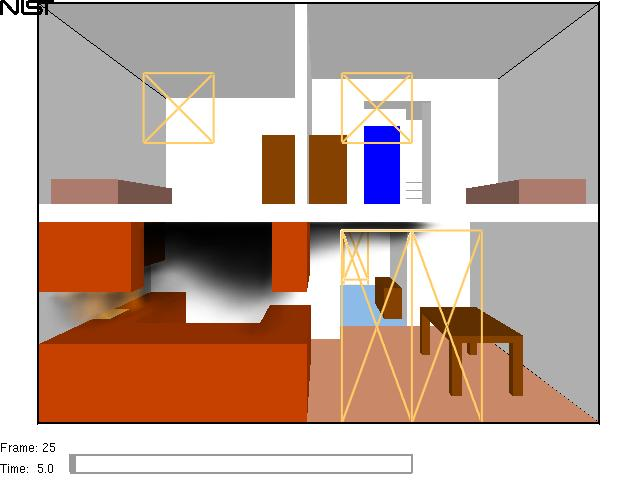
\includegraphics[height=\figheightA]{figures/th_smoke3d_0025}&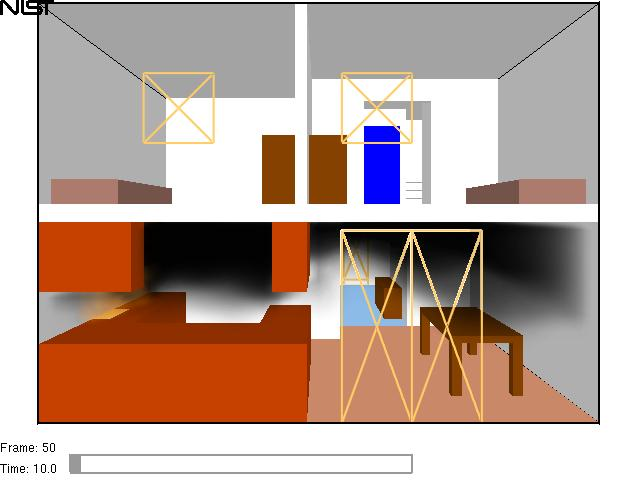
\includegraphics[height=\figheightA]{figures/th_smoke3d_0050}\\
 5.0 s&10.0 s\\
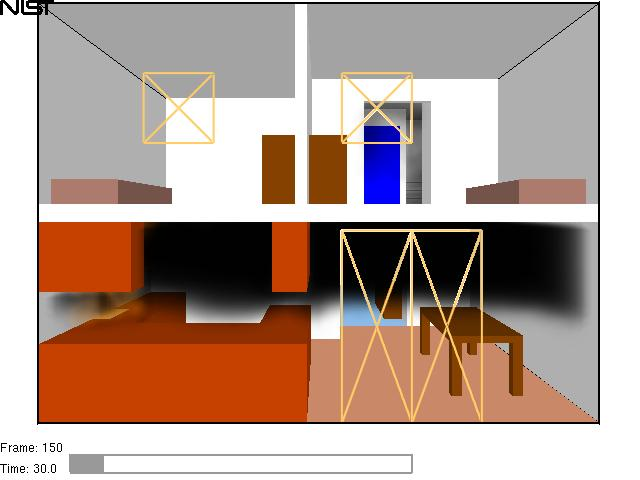
\includegraphics[height=\figheightA]{figures/th_smoke3d_0150}&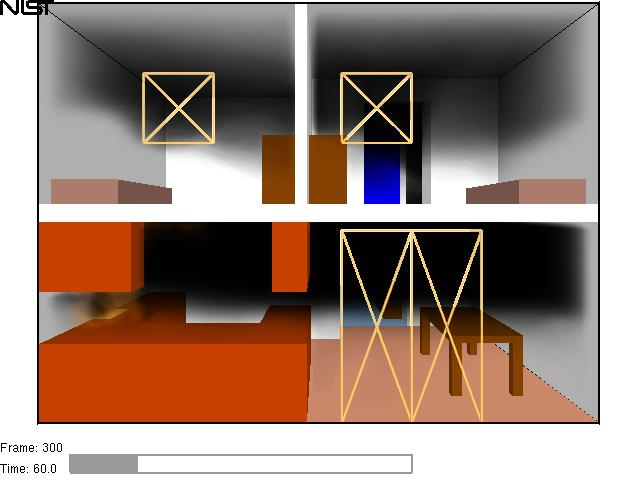
\includegraphics[height=\figheightA]{figures/th_smoke3d_0300}\\
30.0 s&60.0 s\\
\end{tabular}
\end{center}
\caption[Smoke3D file snapshots of a townhouse kitchen fire.]
{Cross section of a townhouse showing first and second floor.
Smoke3d file snapshots at various times in a simulation of a
townhouse kitchen fire.
  }
\label{figsmoke3d}%
\end{figure}

\section{Tracer Particles - Particle Files}

\renewcommand{\figheight}{1.4in}

Particle files contain the locations of tracer particles used to
visualize the flow field. Figure
\ref{figparticle} shows several snapshots of a developing kitchen
fire visualized by using particles where particles are colored
black. If present, sprinkler water droplets would be colored blue.
Particles are stored in files ending with the extension {\tt
.part} and are displayed by selecting the entry from the
\loadmenu\ menu.  Figure \ref{figstreak} shows a snapshot of the same kitchen fire using streak lines instead of particles.  The streaks begin at 6 s and end at 10 s.
This is a good way to show motion using a static image.

\begin{figure}[\figoptions]
\begin{center}
\begin{tabular}{cc}
 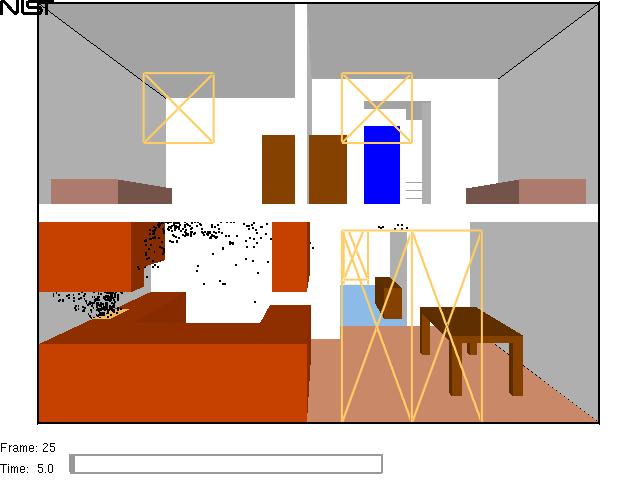
\includegraphics[height=\figheightA]{figures/th_part_0025}&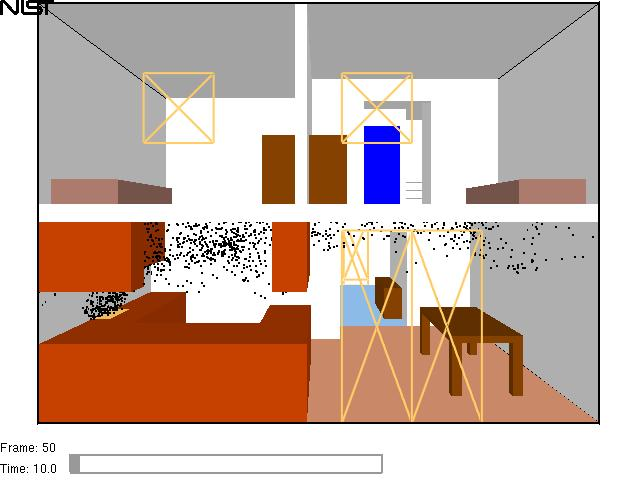
\includegraphics[height=\figheightA]{figures/th_part_0050}\\
 5.0 s&10.0 s\\
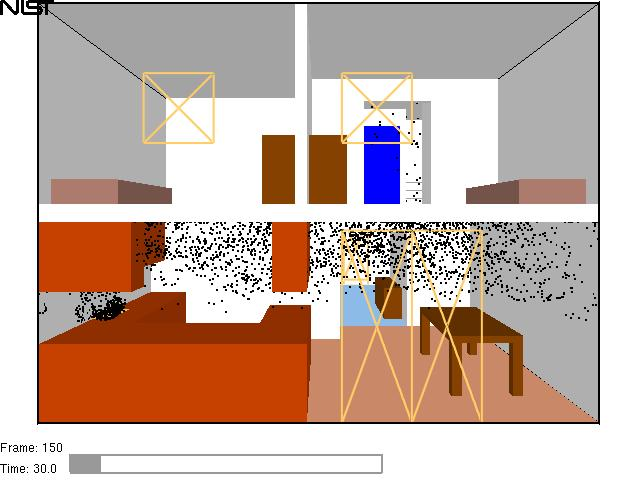
\includegraphics[height=\figheightA]{figures/th_part_0150}&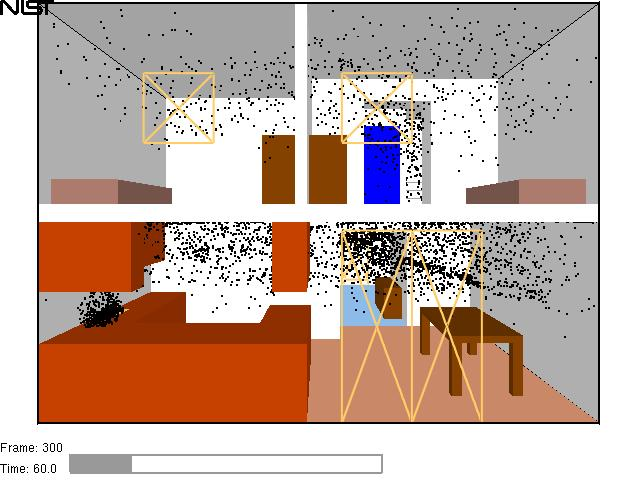
\includegraphics[height=\figheightA]{figures/th_part_0300}\\
30.0 s&60.0 s\\
\end{tabular}
\end{center}

\caption[Particle file snapshots of a townhouse kitchen fire.]
{Cross section of a townhouse showing first and second floor.
Particle file snapshots at four times during the simulation of a
townhouse kitchen fire.}
\label{figparticle}%
\end{figure}

\begin{figure}[\figoptions]
\begin{center}
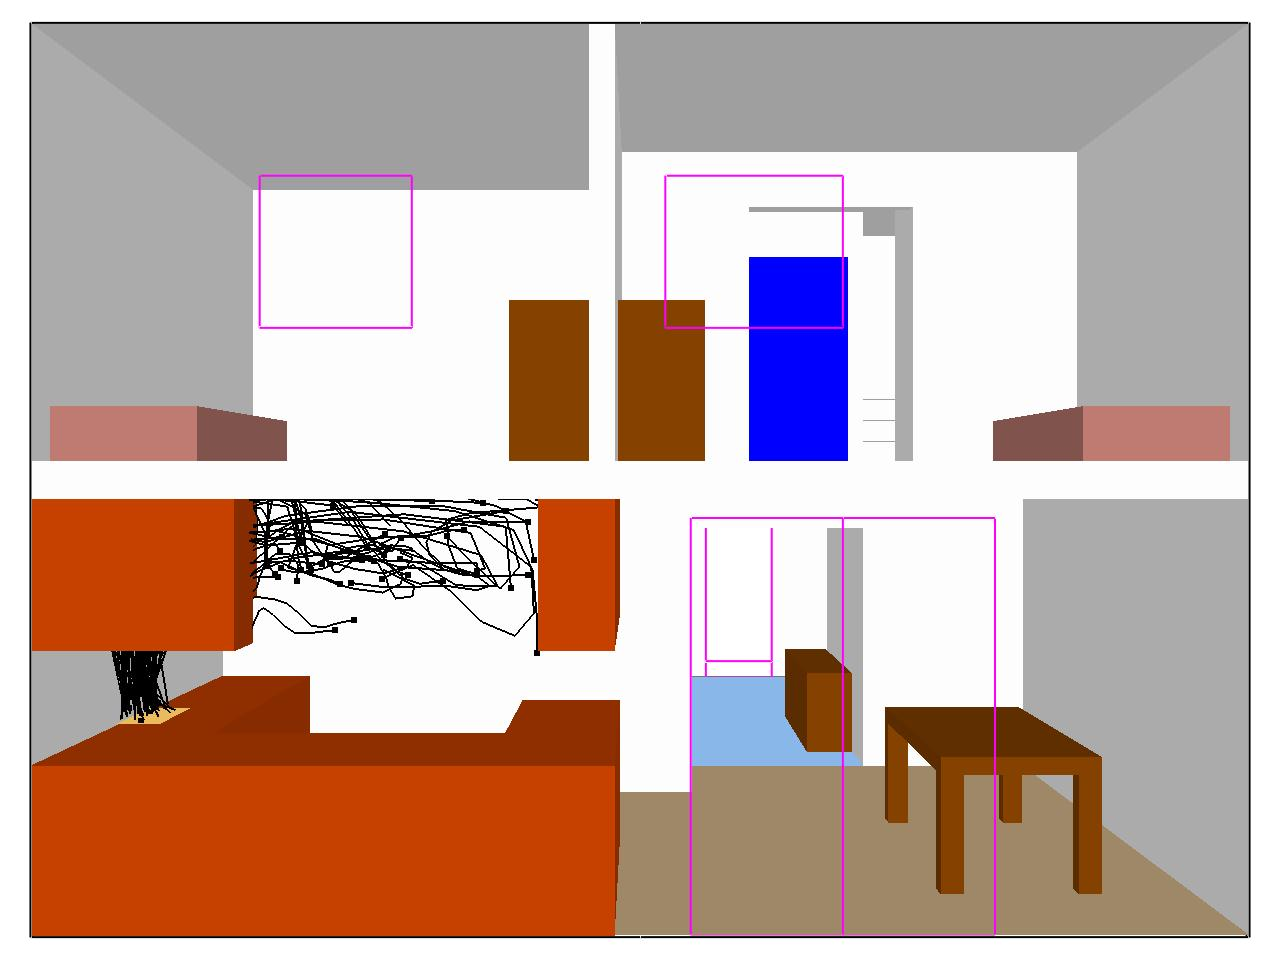
\includegraphics[height=4.0in]{figures/th6_streak}
\end{center}

\caption[Streak lines showing particle paths from 6 to 10 seconds in a townhouse kitchen fire.]
{Cross section of a townhouse showing first and second floor.
Streak lines showing particle paths from 6 to 10 seconds in a townhouse kitchen fire.}
\label{figstreak}%
\end{figure}

\section{2D Shaded Contours - Slice Files}Slice files contain
results recorded within a rectangular array of grid points at each
recorded time step. Continuously shaded contours are drawn for
simulation quantities such as temperature, gas velocity and heat
release rate. All or part of a plane is selected when setting up
the \fds\ input data file. Figure \ref{figslice} shows several
snapshots of a vertical animated slice where the slice is colored
according to gas temperature. Slice files have file names with
extension {\tt .sf} and are displayed by selecting the desired
entry from the \loadmenu\ menu.

\begin{figure}[\figoptions]
\begin{center}
\begin{tabular}{ccc}
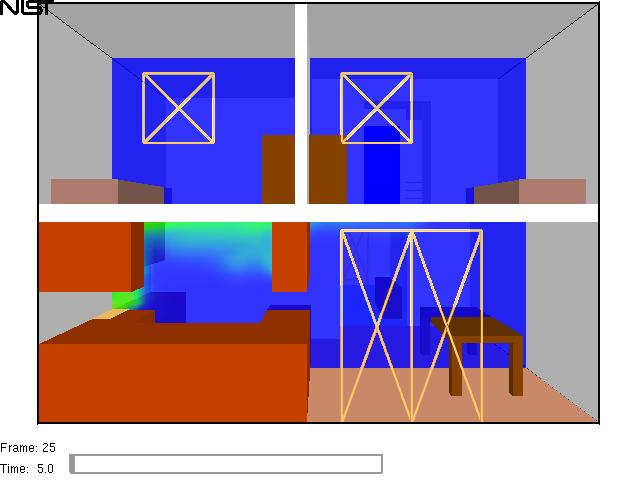
\includegraphics[height=\figheightAbar]{figures/th_slice_0025}&
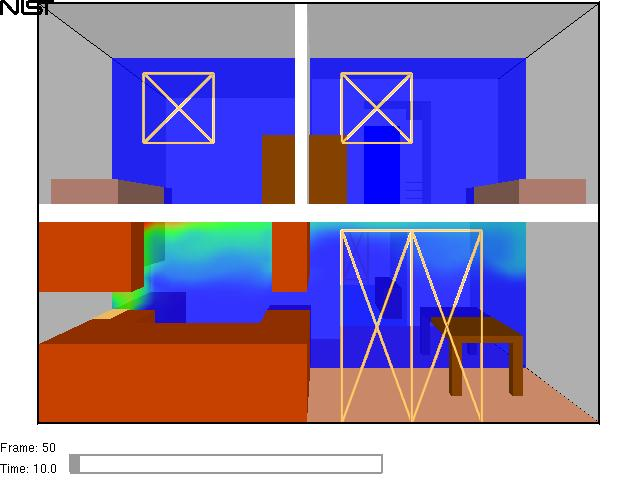
\includegraphics[height=\figheightAbar]{figures/th_slice_0050}\\
5.0 s&10.0 s\\
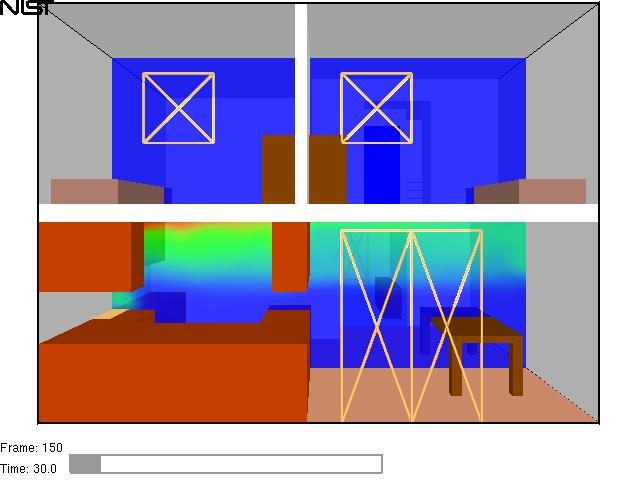
\includegraphics[height=\figheightAbar]{figures/th_slice_0150}&
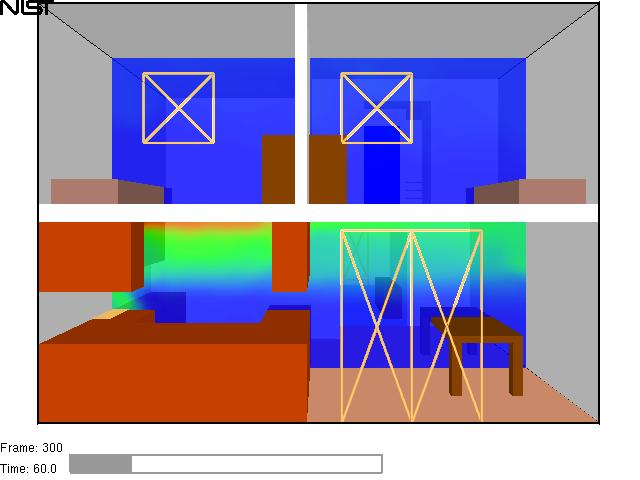
\includegraphics[height=\figheightAbar]{figures/th_slice_0300}&\\
30.0 s&60.0 s
&\raisebox{0.0ex}[0pt]{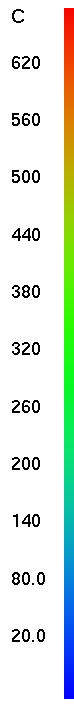
\includegraphics[height=5.0in]{figures/colorbar_20_620}}\\
\end{tabular}
\caption [Slice file snapshots of shaded temperature contours.]
{Slice file snapshots of shaded temperature contours at various
times in a simulation. These contours were generated by adding
``{\tt \&SLCF PBY=1.5,QUANTITY='TEMPERATURE' /}'' to the FDS input
file. }
\label{figslice}%
\end{center}
\end{figure}


\indent To specify in FDS a vertical slice 1.5~m from the $y=0$
boundary colored by temperature, use the line:
\begin{verbatim}
&SLCF PBY=1.5 QUANTITY='TEMPERATURE' /
\end{verbatim}
Other quantities that can be specified are given in Table
\ref{tablegas}. A more complete list may be found in Ref.
\cite{FDS_Users_Guide_4}.

\paragraph{New data coloring}Smokeview uses a new more precise method for coloring data occurring in
slice, boundary and PLOT3D files. This is illustrated in Figure \ref{fignewslice}.  The colors are
now crisper and sharper, more accurately representing the
underlying data. This is most noticeable when selecting the
colorbar with the mouse. As before this causes a portion of the
colorbar to turn black and the corresponding region in the scene
to also turn black.  Now the black color is accurate to the pixel
so this feature could be used to highlight regions of interest.
Data is colored using 1D textures rather than coloring vertices.

\begin{figure}[\figoptions]
\begin{center}
\begin{tabular}{ccc}
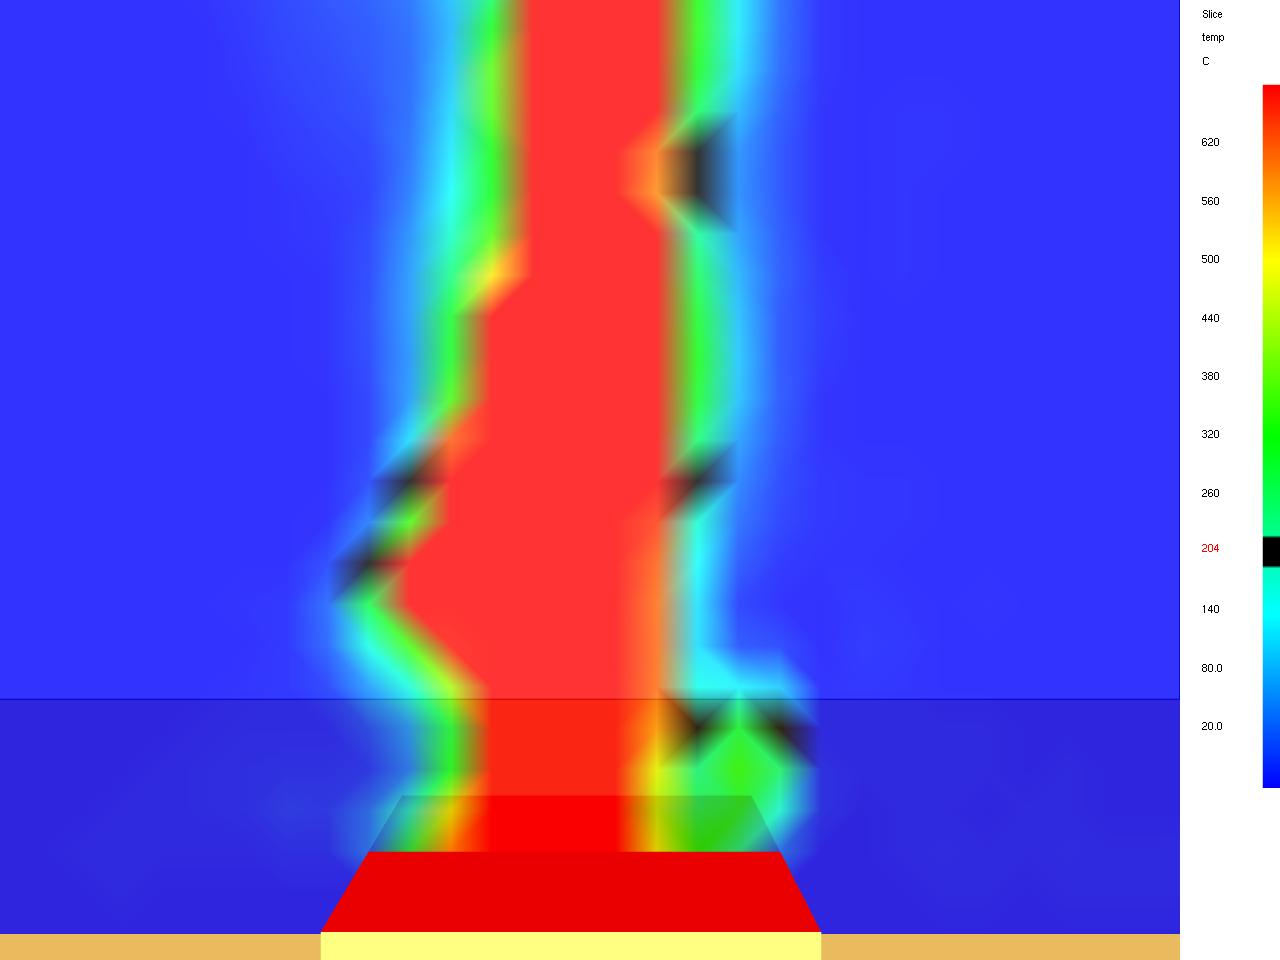
\includegraphics[height=\figheightA]{figures/plume5_sf_bad}&
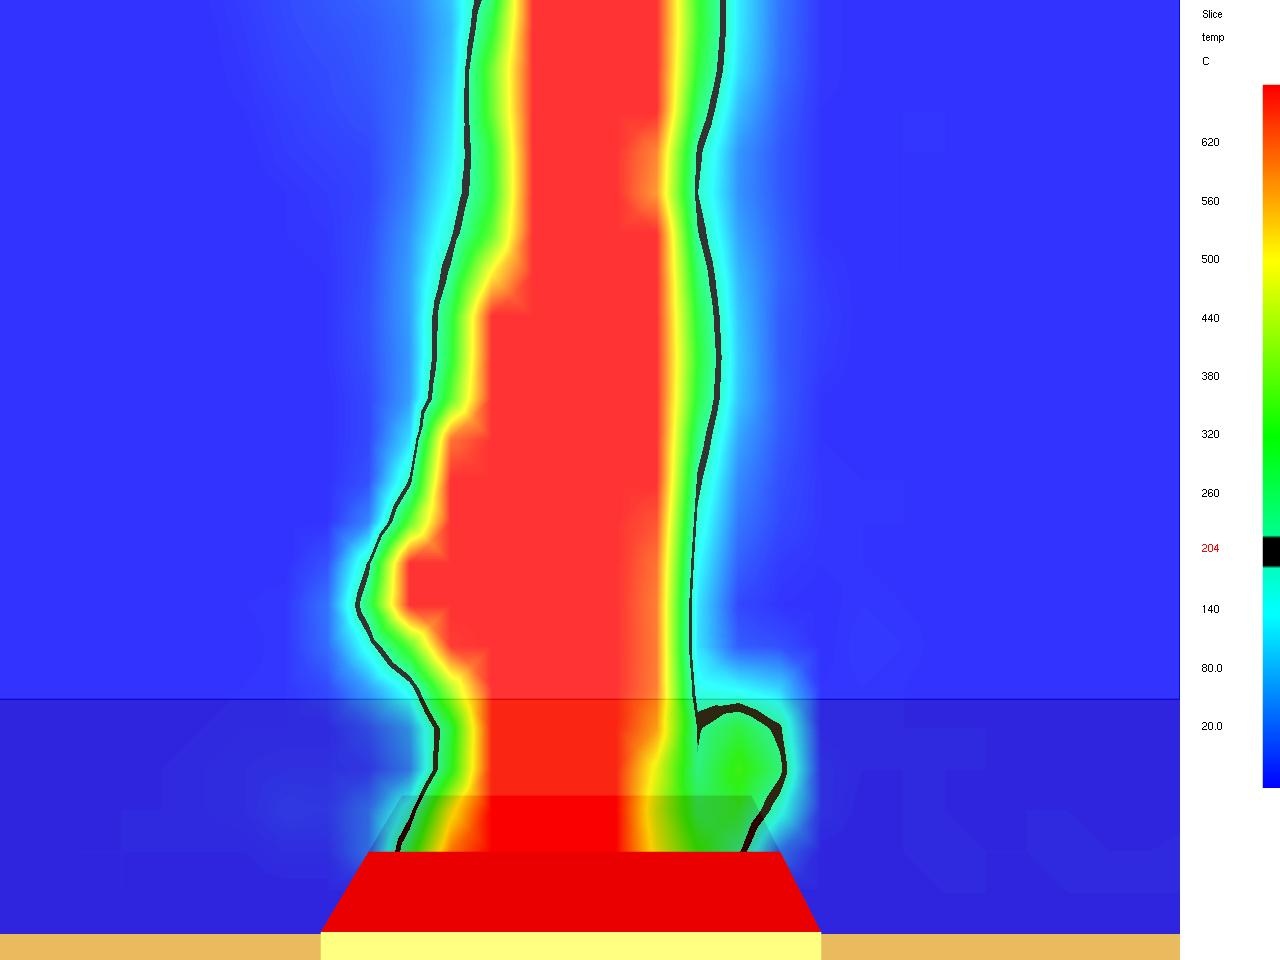
\includegraphics[height=\figheightA]{figures/plume5_sf_good}\\
interpolate colors&interpolate 1D texture color bar\\
\end{tabular}
\caption [Slice file snapshots illustrating old and new method for
coloring data.] {Slice file snapshots illustrating old and new
method for coloring data.}
\label{fignewslice}%
\end{center}
\end{figure}

\paragraph{3D Slice Files}
The user may now visualize a 3D region of data using slice files.
The slices may be moved from one plane to the next just as with
PLOT3D files (using up/down cursor keys or page up/page down
keys).  To specify in FDS a cube of data from 1.0 to 2.0 in each
of the X, Y and Z directions, use the line:
\begin{verbatim}
&SLCF XB=1.0,2.0,1.0,2.0,1.0,2.0 QUANTITY='TEMPERATURE' /
\end{verbatim}

\begin{table}[\figoptions]
\caption[Some output quantities used to generate slice and Plot3D
visualizations.]{Some output quantities used to generate slice and
Plot3D visualizations.  A more complete list may be found in
Ref.\cite{FDS_Users_Guide_4}}
\begin{center}
\begin{tabular}{|l|l|l|}
\hline
Quantity                   &  Description             & Units               \\ \hline \hline
{\tt DENSITY}              & density                  & kg/m$^3$            \\ \hline
{\tt TEMPERATURE}          & gas temperature          & \degC               \\ \hline
{\tt U-VELOCITY}           & velocity component       & m/s                 \\ \hline
{\tt V-VELOCITY}           & velocity component       & m/s                 \\ \hline
{\tt W-VELOCITY}           & velocity component       & m/s                 \\ \hline
{\tt VELOCITY}             & velocity magnitude       & m/s                 \\ \hline
\end{tabular}
\end{center}
\label{tablegas}
\end{table}

Animated vectors are displayed using data contained in two or more
slice files.  The direction and length of the vectors are
determined from the $U$, $V$ and/or $W$ velocity slice files. The
vector colors are determined from the file (such as temperature)
selected from the \loadmenu\ menu. Figure \ref{figvslice} shows a
sequence of vector slices corresponding to the shaded temperature
contours found in Figure \ref{figslice}.

\begin{figure}[\figoptions]
\begin{center}
\begin{tabular}{ccc}
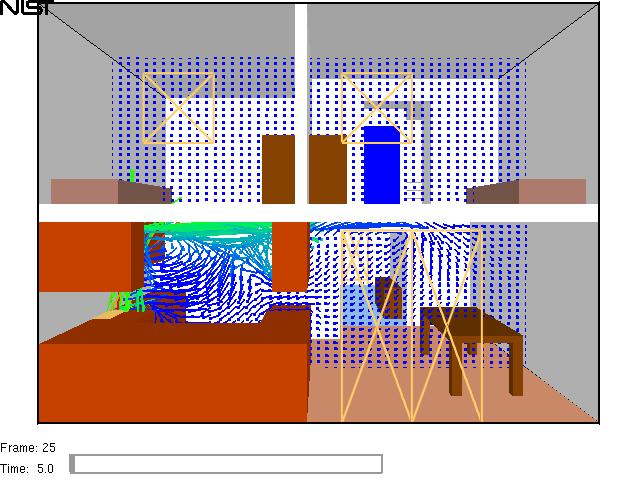
\includegraphics[height=\figheightAbar]{figures/th_vslice_0025}&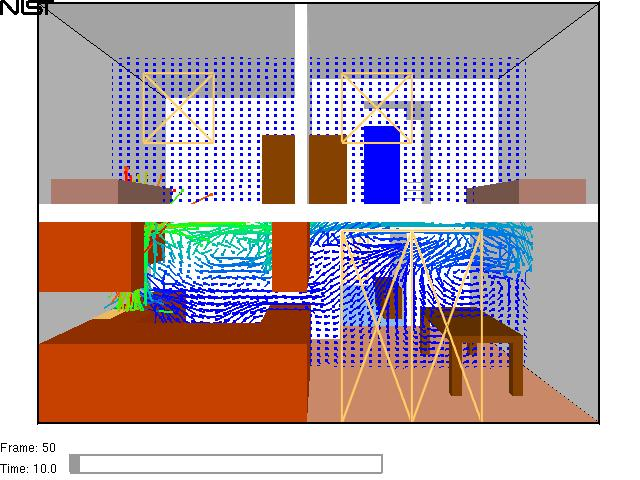
\includegraphics[height=\figheightAbar]{figures/th_vslice_0050}\\
5.0 s&10.0 s\\
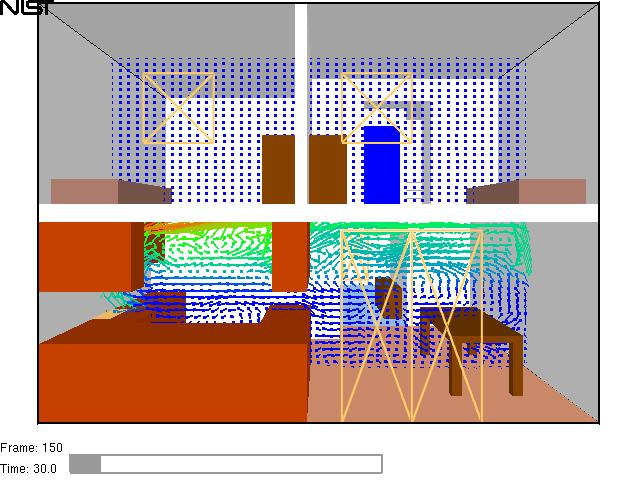
\includegraphics[height=\figheightAbar]{figures/th_vslice_0150}&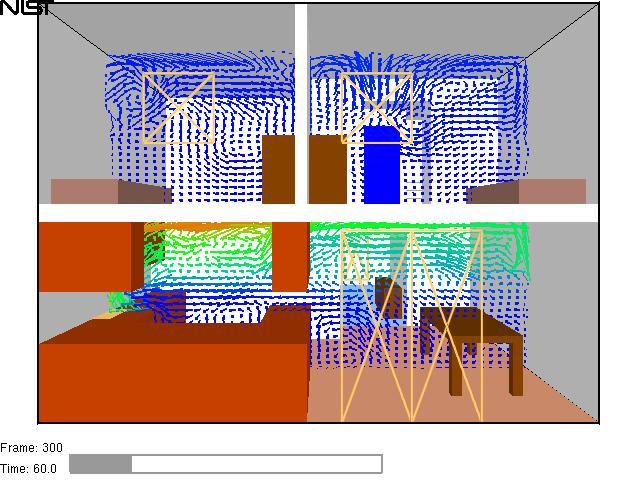
\includegraphics[height=\figheightAbar]{figures/th_vslice_0300}\\
30.0 s&60.0 s
&\raisebox{0.0ex}[0pt]{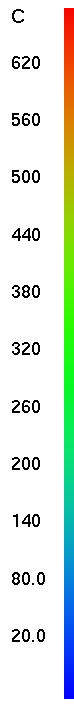
\includegraphics[height=5.0in]{figures/colorbar_20_620}}\\
\end{tabular}
\end{center}
\caption [Vector slice file snapshots of shaded vector plots.]
{Vector slice file snapshots of shaded vector plots. These vector
plots were generated by using ``{\tt \&SLCF
PBY=1.5,QUANTITY='TEMPERATURE',VECTOR=.TRUE. /}''.}
\label{figvslice}%
\end{figure}

To generate the extra velocity files needed to view vector
animations, add {\tt VECTOR=.TRUE.} to the above {\tt
\&SLCF} line to obtain:
\begin{verbatim}
&SLCF PBY=1.50,QUANTITY='TEMPERATURE',VECTOR=.TRUE. /
\end{verbatim}

\section{2D Shaded Contours on Solid Surfaces - Boundary
Files}Boundary files contain simulation data recorded at blockage
or wall surfaces. Continuously shaded contours are drawn for
quantities such as wall surface temperature, radiative flux, \etc.
Figure \ref{figboundary} shows several snapshots of a boundary
file animation where the surfaces are colored according to their
temperature. Boundary files have file names with extension {\tt
.bf} and are displayed by selecting the desired entry from the
\loadmenu\  menu.
\begin{figure}[\figoptions]
\begin{center}
\begin{tabular}{ccc}
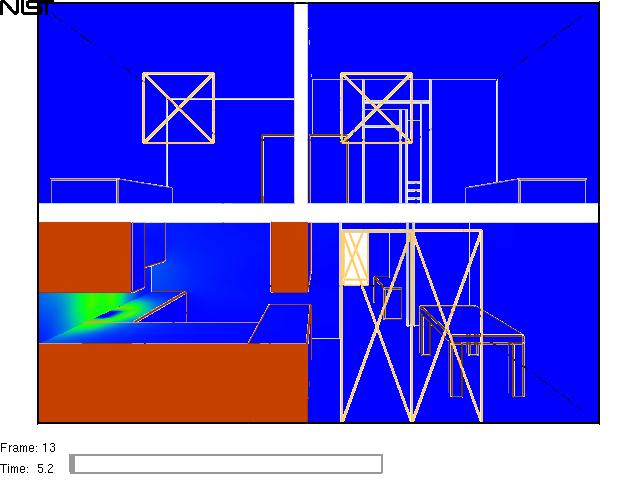
\includegraphics[height=\figheightAbar]{figures/th_bound_0025}&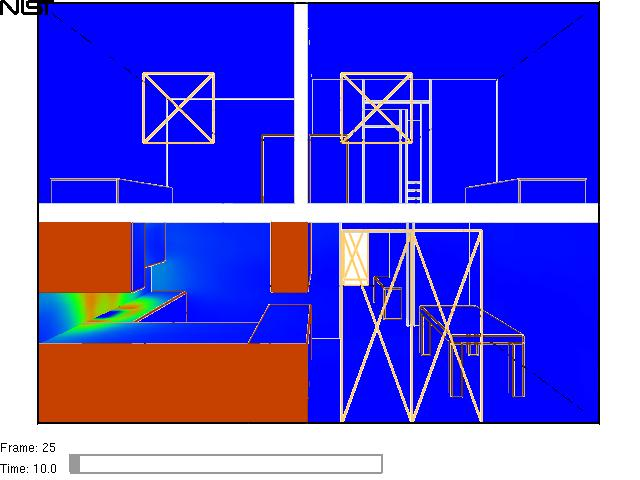
\includegraphics[height=\figheightAbar]{figures/th_bound_0050}\\
5.0 s&10.0 s\\
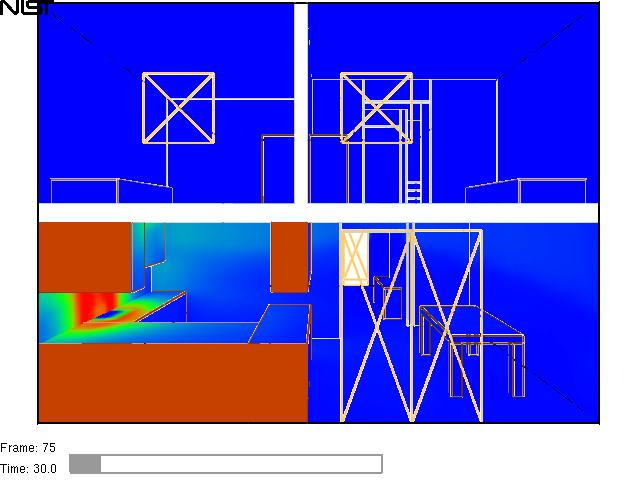
\includegraphics[height=\figheightAbar]{figures/th_bound_0150}&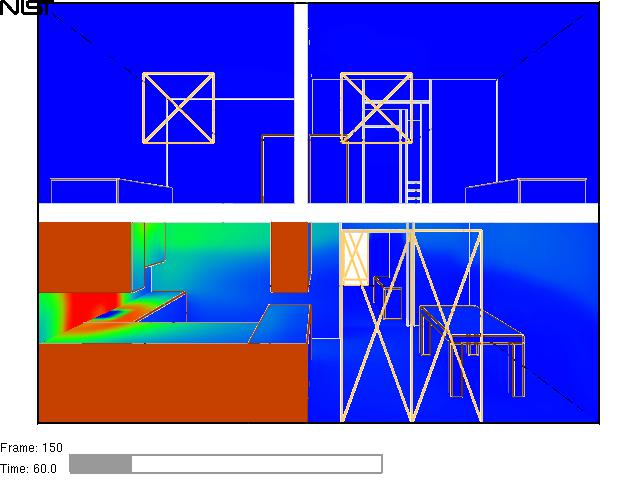
\includegraphics[height=\figheightAbar]{figures/th_bound_0300}\\
30.0 s&60.0 s
&\raisebox{0.0ex}[0pt]{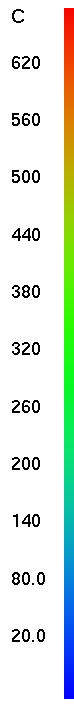
\includegraphics[height=5.0in]{figures/colorbar_20_620}}\\
\end{tabular}
\end{center}
\caption [Boundary file snapshots of shaded wall temperatures
contours.] {Boundary file snapshots of shaded wall temperatures.
These snapshots were generated by using ``{\tt\&BNDF
QUANTITY='WALL\_TEMPERATURE'/}''. }
\label{figboundary}%
\end{figure}
\begin{figure}[\figoptions]
\begin{center}
\begin{tabular}{cc}
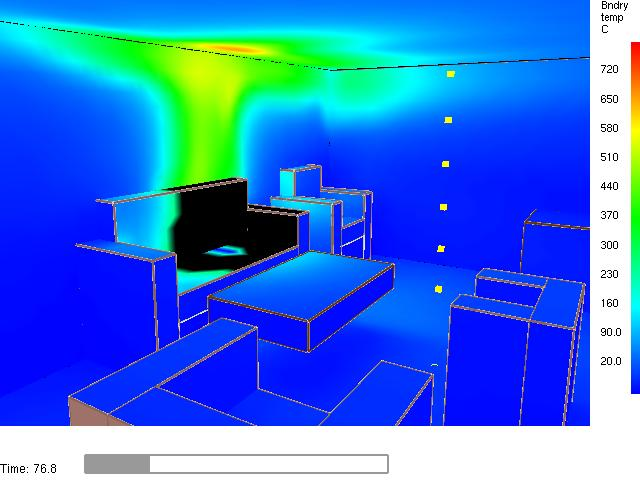
\includegraphics[height=\figheightA]{figures/roomfireb}&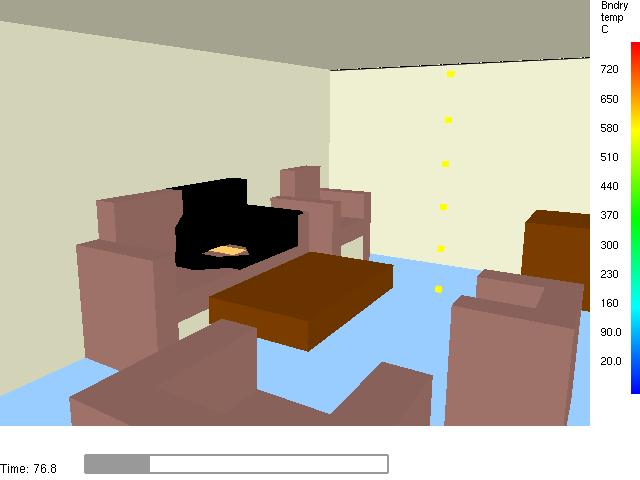
\includegraphics[height=\figheightA]{figures/roomfirec}\\
Showing Ignited Surfaces&Showing Only Ignited Surfaces\\
\end{tabular}
\end{center}
\caption{Boundary file snapshots showing ignited surfaces}
\label{figboundary2}%
\end{figure}

A boundary file containing wall temperature data may be
generated by using:
\begin{verbatim}
&BNDF 'WALL_TEMPERATURE' /
\end{verbatim}
Loading a boundary file is a memory intensive operation.  The
entire boundary file is read in to determine the minimum and
maximum data values.  These bounds are then used to convert four
byte floats to one byte color indices.  To drastically reduce the
memory requirements, simply specify the minimum and maximum data
bounds using the \setbounds\ dialog box.  This should be done
before loading the boundary file data.  When this is done, memory
for the boundary file data is allocated for only one time step
rather than for all time steps.

\paragraph{Highlighting Ignited Surfaces}
Wall temperature boundary file data may be colored black where
temperatures exceed the ignition temperature of the underlying
surface where the ignition temperature is defined on the FDS
\&SURF line. This is activated by selecting the {\em Show Ignition}\
check box in the Set Bounds dialog box.  If one also selects the
{\em how Only Ignition}\ check box then the ignited material is
drawn black but the rest of the boundary file is not drawn.

 Table \ref{tableflux} gives other quantities
that can be specified on a {\tt \&BNDF} line. A more complete list
of quantities is given in Ref. \cite{FDS_Users_Guide_4}.

\begin{table}[\figoptions]
\begin{center}
\caption[Some output quantities used to generate boundary file
visualizations.]{Some output quantities used to generate boundary
file visualizations. A more complete list may be found in
Ref.\cite{FDS_Users_Guide_4}}
\begin{tabular}{|l|l|l|}
\hline
Quantity                 & Description                     & Units          \\ \hline \hline
{\tt RADIATIVE\_FLUX}    & radiative flux                  & kW/m$^2$       \\ \hline
{\tt CONVECTIVE\_FLUX}   & convective flux                 & kW/m$^2$       \\ \hline
{\tt WALL\_TEMPERATURE}  & wall temperature                & \degC          \\ \hline
\end{tabular}
\label{tableflux}
\end{center}
\end{table}

\section{3D Contours - Isosurface Files}
\begin{figure}[\figoptions]
\begin{center}
\begin{tabular}{cc}
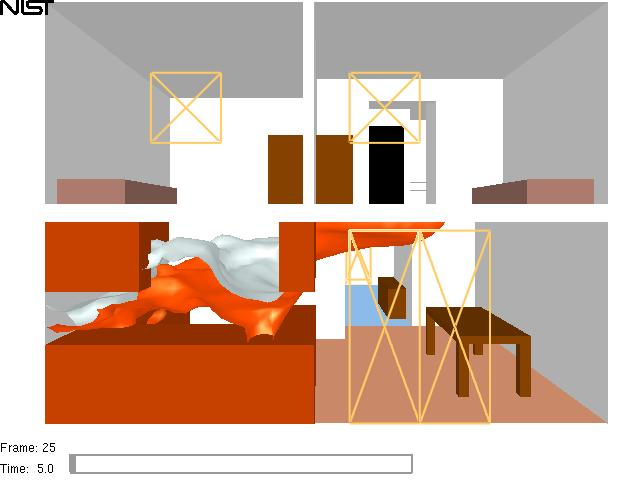
\includegraphics[height=\figheightA]{figures/thouse3d4_iso_0025}&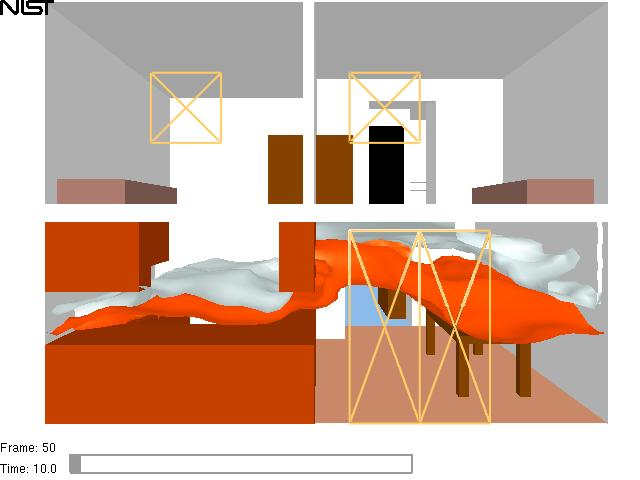
\includegraphics[height=\figheightA]{figures/thouse3d4_iso_0050}\\
5.0 s&10.0 s\\
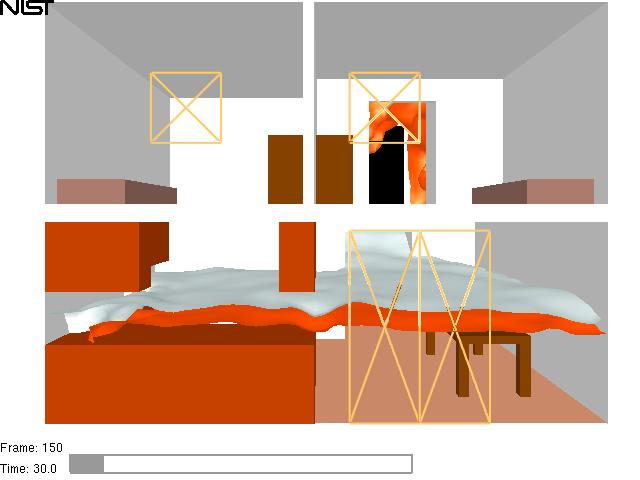
\includegraphics[height=\figheightA]{figures/thouse3d4_iso_0150}&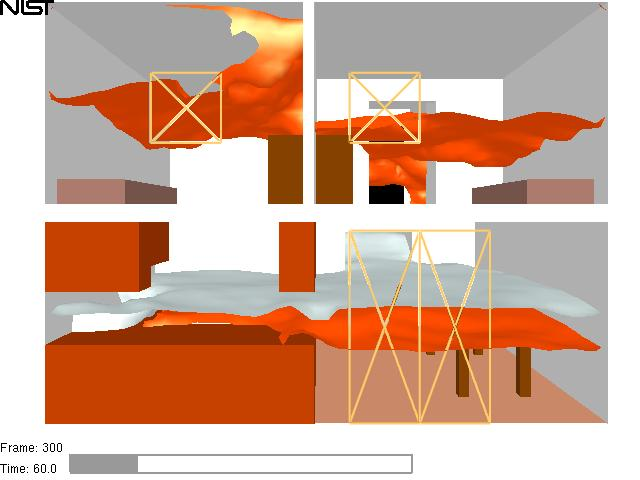
\includegraphics[height=\figheightA]{figures/thouse3d4_iso_0300}\\
30.0 s&60.0 s
\end{tabular}
\end{center}
\caption [Isosurface file snapshots of temperature levels. ]

{ Isosurface file snapshots of temperature levels. The orange
surface is drawn where the air/smoke temperature is 30~\degC\ and
the white surface is drawn where the air/smoke temperature is
100~\degC. These snapshots were generated by adding ``{\tt\&ISOF
QUANTITY='TEMPERATURE',VALUE(1)=30.0,VALUE(2)=100.0 /}'' to the
FDS input file.}
\label{figiso}%
\end{figure}

The surface where a quantity such as temperature attains a given
value is called an isosurface. An isosurface is also called a
level surface or 3D contour. Isosurface files contain data
specifying isosurface locations for a given quantity at one or
more levels. These surfaces are represented as triangles.
Isosurface files have file names with extension .iso and are
displayed by selecting the desired entry from the \loadmenu\ menu.

Isosurfaces are specified in the \fds\ input file with the {\tt
\&ISOF} keyword.  To specify isosurfaces for temperatures of
30\degC\ and 100\degC\ as illustrated in Figure \ref{figiso} add
the line:
\begin{verbatim}
&ISOF QUANTITY='TEMPERATURE',VALUE(1)=30.0,VALUE(2)=100.0 /
\end{verbatim}
to the FDS input file. Other quantities may be specified using
values given in Table \ref{tablegas}. A more complete list may be
found in Ref. \cite{FDS_Users_Guide_4}

\section{Static Data - Plot3D Files} Data stored in Plot3D files
use a format developed by NASA~\cite{PLOT3D} and are used by many
CFD programs for representing simulation results. Plot3D files
store five data values at each grid cell. \FDS\ uses Plot3D files
to store temperature, three components of velocity (U, V, W) and
heat release rate. Other quantities may be stored if desired.

An \fds\ simulation will typically create Plot3D files at several
specified times throughout the simulation. Plot3D data is
visualized in three ways: as 2D contours, vector plots and
isosurfaces. Figure \ref{fig2dcontour}a shows an example of a 2D
Plot3D contour. Vector plots may be viewed if one or more of the
U,V and W velocity components are stored in the Plot3D file. The
vector length and direction show the direction and relative speed
of the fluid flow. The vector colors show a scalar fluid quantity
such as temperature. Figure \ref{figvector2}b shows vectors in a
doorway. The vector lengths may be adjusted by depressing the
``a'' key.  Note the hot flow (red color) leaving the fire room in
the upper part of the door and the cool flow (blue color) entering
fire room in the lower part of the door. Figure \ref{fig3dcontour}
gives an example of isosurfaces for two different temperature
levels. Plot3D data are stored in files with extension {\tt .q} .

\begin{figure}[\figoptions]
\begin{center}
\begin{tabular}{cc}
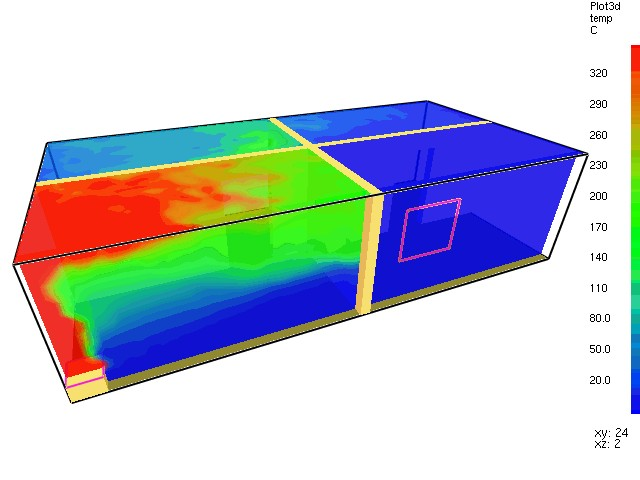
\includegraphics[height=2.0in]{figures/roomfire_plot3d}
&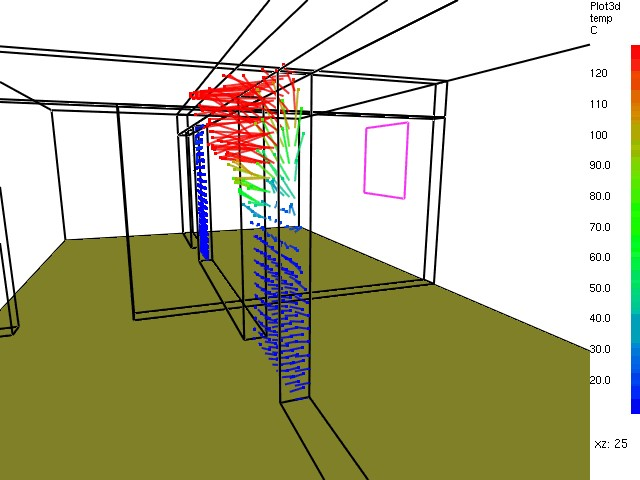
\includegraphics[height=2.0in]{figures/roomfire_plot3dv}\\
a)

\parbox[t]{2.5in}{shaded 2D temperature contour plots in a vertical plane through the fire and a
horizontal plane below the ceiling}
&
b)
\parbox[t]{2.5in}{shaded temperature vector plot in a vertical plane through the doorway.
The ``a'' key may be depressed to alter the vector sizes.
The ``s'' key may be depressed to alter the number of vectors displayed.
}
\end{tabular}
\end{center}
\caption{Plot3D contour and vector plot examples.  }
\label{fig2dcontour}%
\label{figvector2}
\end{figure}

\begin{figure}[\figoptions]
\begin{center}
\begin{tabular}{cc}
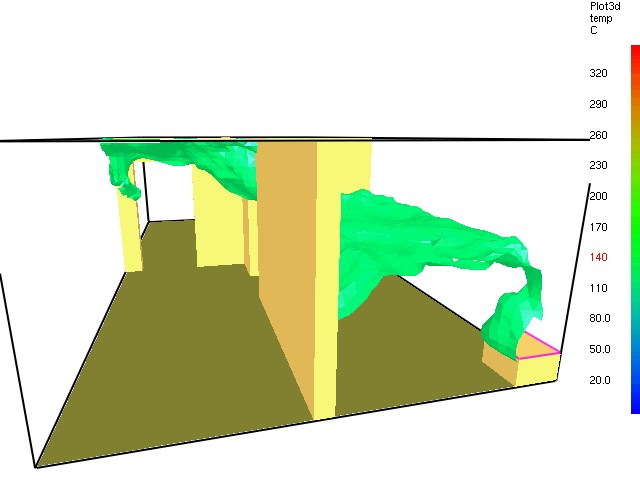
\includegraphics[height=2.0in]{figures/roomfire_iso2}
&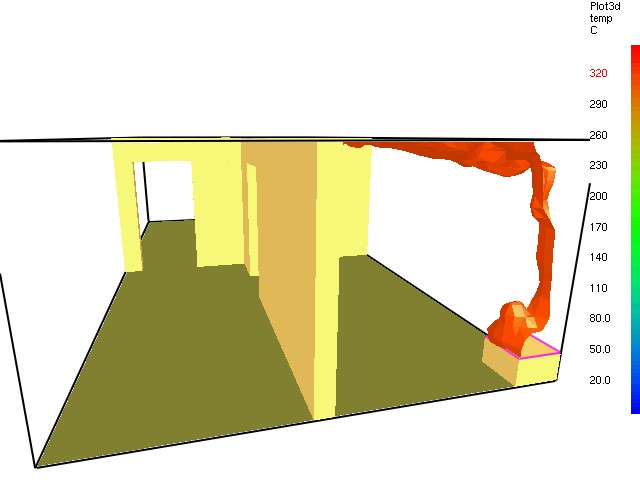
\includegraphics[height=2.0in]{figures/roomfire_iso1}\\
a) temperature isosurface at 140 \degC&b) temperature
isosurface at 320 \degC
\end{tabular}
\end{center}
\caption{Plot3D isocontour example.}
\label{fig3dcontour}%
\end{figure}

\section{Zone Fire Modeling Data - PLT Files}
The zone fire model CFAST\cite{Jones:2004A} creates files that Smokeview may use to visualize the case being simulated.
Smokeview visualizes the geometric layout of the scenario.  It also visualizes the layer interface heights, upper layer temperature and vent flow.  The vent flow
is computed internally in Smokeview using the same equations and data (pressure at floor, layer interface  heights and lower/upper layer temperatures) as used by CFAST.
The vent flow colors represent the temperature of the flow origin, the length vent flow region is proportional to the flow velocity.  Plumes are represented as inverted cones with heights determined using the CFAST reported heat release rate and
the same correlation that CFAST uses.
A Smokeview view of the one room sample case that comes with the CFAST installation is illustrated in Figure \ref{figcfast}.

\begin{figure}[\figoptions]
\begin{center}
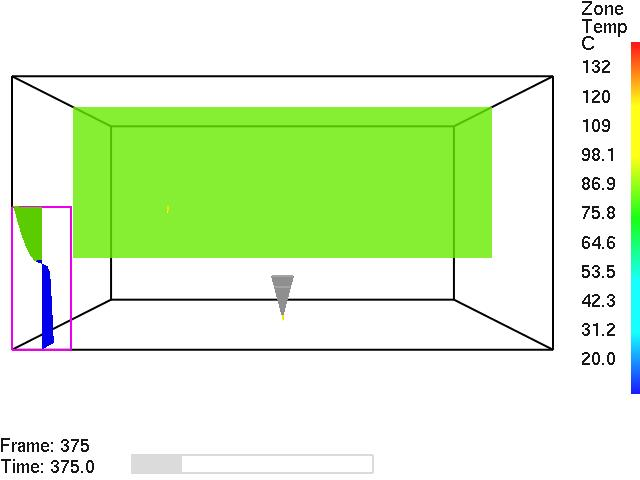
\includegraphics[height=3.5in]{figures/standard_0375}
\end{center}
\caption{CFAST 6.0 Standard case showing upper layer and vent flow at 375 s.}
\label{figcfast}%
\end{figure}
%---------------------------------------------------------------------------------
%------------------------ Advanced Features --------------------------------------
%---------------------------------------------------------------------------------

\chapter{Advanced Features}

\section{Manipulating the Scene Automatically - The Touring
Option}

\begin{figure}[\figoptions]
\begin{center}
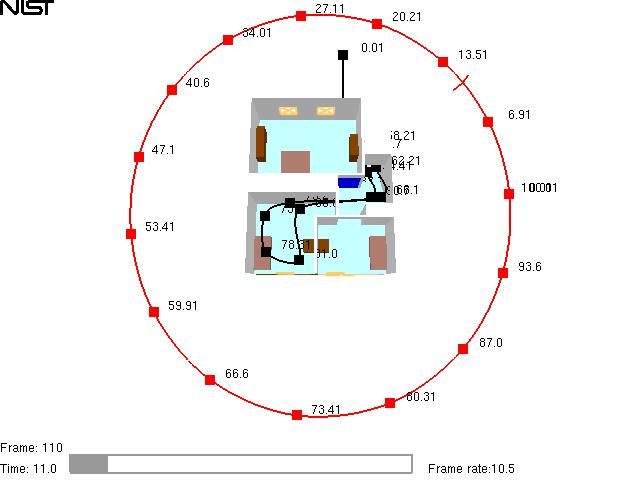
\includegraphics[width=4.4444in]{FIGURES/figTOUREXAMPLE}\\
\end{center}
\caption[Overhead view of the townhouse example showing the
default {\em Circle}\ tour and a user defined tour.]{Overhead view of
townhouse example showing the default {\em Circle}\ tour and a user
defined tour.  The square dots indicate the keyframe locations.
Keyframes may be edited using the Touring or Advanced Touring
dialog boxes.}
 \label{figTOUREXAMPLE}
\end{figure}

\begin{figure}[\figoptions]
\begin{center}
\begin{tabular}{cc}
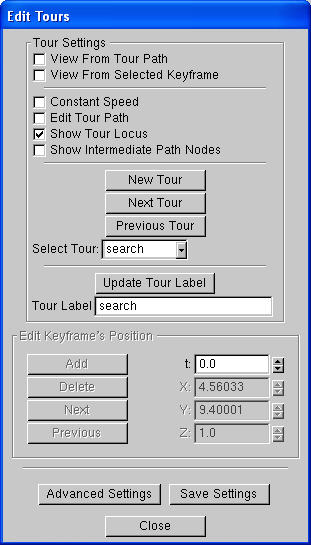
\includegraphics[width=2.159722in]{FIGURES/figTOUR}&
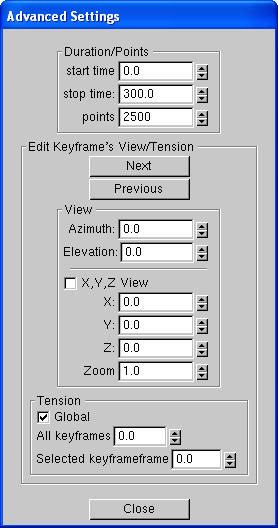
\includegraphics[width=1.93055in]{FIGURES/figADVANCEDTOUR}\\
a) basic options&b) advanced options\\
\end{tabular}
\end{center}
\caption[Touring dialog boxes]{The Touring dialog boxes may be
used to select tours or keyframes, change the position or view
direction at each keyframe and change the tension of the tour
path. }
 \label{figTOUR}
\end{figure}

The touring option allows one to specify arbitrary paths or tours
through or around a Smokeview scene.  One may then view the
scenario from the vantage point of an observer moving along one of
these paths.  Alternatively, one may observe the motion along all
of the paths simultaneously from an external vantage point. These
paths may be used to represent the movement of building occupants
or first responders during a fire incident, or to highlight key
portions or features of a scenario during presentations.  A tour
may also be used to observe time dependent portions of the
scenario such as blockage/vent opening and closings.  The default
view direction is towards the direction of motion.  The view
direction and path tension may be changed with the {\bf Advanced
Settings}\ dialog box.

When Smokeview starts up it creates a tour, called the {\em circle
tour}\ which surrounds the scene.  The {\em circle}\ tour and a user
defined tour are illustrated in Figure \ref{figTOUREXAMPLE}. The
circle tour is similar to the \tourmenu\ menu option found in
earlier versions of Smokeview. The user may modify the {\em circle}\
tour or define their own tours by using the {\bf Tour}\ dialog box
illustrated in Figure \ref{figTOUR}. The user places several
points or keyframes in or around the scene. Smokeview creates a
smooth path going through these points.

\paragraph{Tour Settings}
An existing tour may be modified by selecting it from the {\bf
Select tour:}\ listbox found in the Tour dialog box.  A new tour
may be created by clicking the {\bf Add Tour} button. A newly
created tour goes through the middle of the Smokeview scene
starting at the front left and finishing at the back right. A tour
may also be modified by editing the text entries found in the
{\em local}\ preference file, casename.ini under the {\bf TOUR}\
keyword.

The speed traversed along the tour is determined by the time value
assigned to each keyframe.   If the {\bf Constant Speed}\ checkbox
is checked then these times are determined given the distance
between keyframes and the velocity required to traverse the entire
path in the specified time as given by the {\em start time}\ and
{\em stop time}\ entries found in the {\bf Advanced Settings}\ dialog
box.


Three different methods for viewing the scene may be selected.  To
view the scene from the point of view of the selected tour, check
the {\bf View From Tour Path}\ checkbox. To view the scene from a
keyframe (to see the effect of editing changes), select the {\bf
View From Selected Keyframe}\ checkbox. Unchecking these boxes
returns control of scene movement to the user.

\paragraph{Keyframe Settings}
A keyframe may be selected for editing by either clicking it with
the mouse or by using the {\bf Next} or {\bf Previous} buttons.
Keyframe positions may then be modified by changing data in the t,
X, Y or Z edit boxes. A different view direction may be selected
using the {\bf Advanced Settings}\ dialog box.

A new keyframe is created by clicking the {\bf Add}\ button. It is
formed by averaging the positions and view directions of the
current and next keyframes. If the selected keyframe is the last
one in the tour then a new keyframe  is added beyond the last
keyframe.

A keyframe may be deleted by clicking the {\bf Delete}\ button.
There is no {\bf Delete Tour}\ button. A tour may be deleted by
either deleting all of its keyframes or by deleting its entry in
the casename.ini file.

\paragraph{Advanced Settings}
The {\bf Advanced Settings}\ dialog box is only necessary if one
wishes to override Smokeview's choice of view direction (along the
direction of motion) or tension settings.  This dialog box is
opened by clicking the {\bf Advanced Settings}\ button contained
in the {\bf Keyframe Settings} dialog box.

A view direction may be defined at each keyframe by either setting
direction angles relative to the path (an azimuth and an elevation
angle) or by setting a direction relative to the scene geometry (a
cartesian (X,Y,Z) view direction).

Path relative view directions are enabled by default.  To define a
cartesian view direction, select the {\bf X,Y,Z View}\ check box
and edit the X, Y and Z View edit boxes to change the view
location. To define an path relative view direction, uncheck the
{\bf X,Y,Z View}\ check box and edit the Azimuth and Elevation
edit boxes. Checking the {\bf View From Selected Keyframe}
checkbox allows one to see the effects of the above view changes
from the keyframe being edited. To see the effect of a change in
one of the keyframe's parameters, uncheck the {\bf View From
Selected Keyframe}\ checkbox and position the tour locator
(vertical and horizontal red lines) near the keyframe.  The
horizontal red line always points in the view direction.

Spline tension settings may also be changed using the {\bf
Advanced Settings}\ dialog box, though normally this is not
necessary except when one wishes abrupt rather than smooth path
changes. Kochanek-Bartels\cite{Moller:02} splines (piecewise cubic
Hermite polynomials) are used to represent the tour paths.

The cubic Hermite polynomials for each interval are uniquely
specified using a function and a derivative at both endpoints of
the interval ({\em i.e. 4 data values}).  These derivatives are
computed in terms of three parameters referred to as {\em bias},
{\em continuity} and {\em tension}. Each of these parameters range
from -1 to 1 with a default value of 0. The tension value may be
set for all keyframes at once (by checking the {\bf Global}\
checkbox) or for each keyframe separately.  The bias and
continuity values are set to zero internally by Smokeview.  A
tension value of 0 is set by default, a value of 1 results in a
linear spline.


\paragraph{Setting up a tour}
\begin{figure}[\figoptions]
\begin{center}
\begin{tabular}{cc}
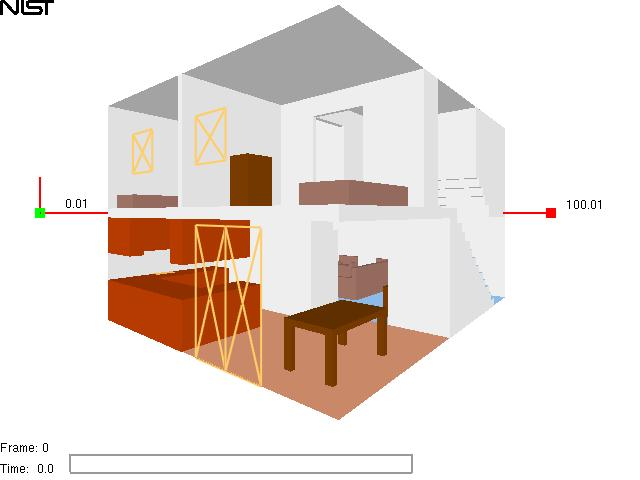
\includegraphics[height=\figheightA]{figures/figTOUR_1}&
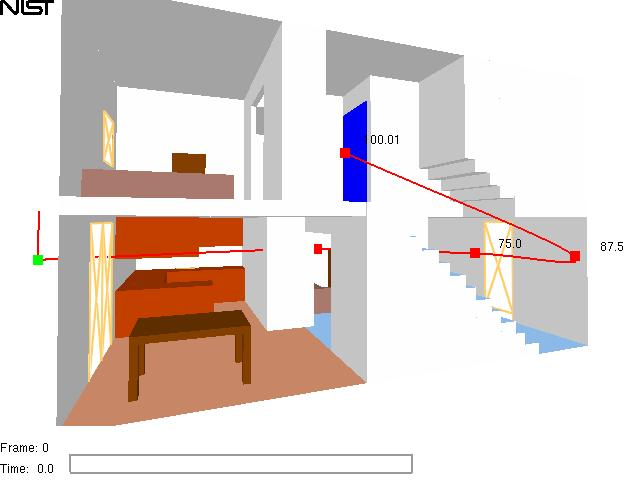
\includegraphics[height=\figheightA]{figures/figTOUR_2}\\
a) Initial tour&b) First and last step set with 5 keyframes\\
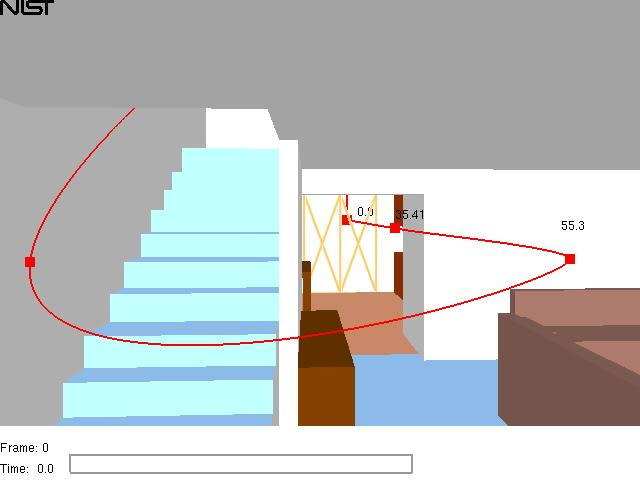
\includegraphics[height=\figheightA]{figures/figTOUR_3}&
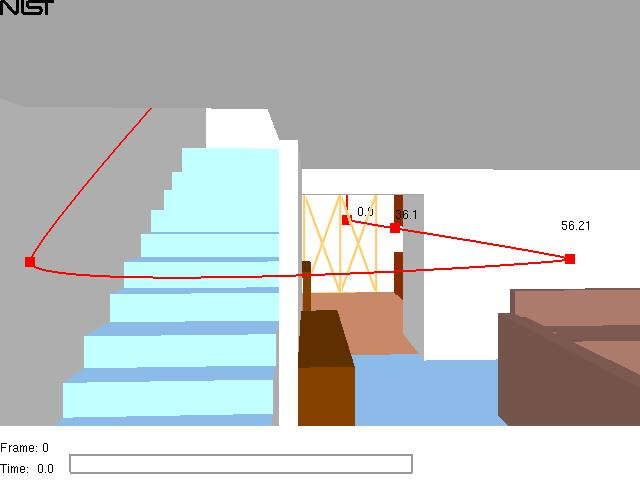
\includegraphics[height=\figheightA]{figures/figTOUR_4}\\
c) All keyframe positions set (tension=0.0)&d) Tension set to 0.75
\end{tabular}
\end{center}
\caption [Tutorial examples for Tour option] {Tutorial examples for Tour option.}
\label{figTutorial}%
\end{figure}


The following steps give a simple example of setting up a tour in the
townhouse scenario.  The tour will begin at the back of the house,
go towards the front door and then end at the top of the stairs.
These steps are illustrated in Figure \ref{figTutorial}.

\begin{enumerate}
\item Start by clicking the \frameit{Dialog$>$Tours...}\ menu item
which opens up the \frameit{Edit Tours}\ dialog box.

\item  Click on the \frameit{New Tour}\ button in the Tour dialog
box. This creates a tour, illustrated in Figure
\ref{figTutorial}a, starting at the front left of the scene and
ending at the back right. This tour has two keyframes.  The
elevation of each keyframe is halfway between the bottom and top
of the scene.

\item Click on the \frameit{Edit Tour Path} checkbox. This
activates buttons that allows the user to edit the properties of
each individual keyframe. Click on the square dot at the back of
the townhouse. This is the first keyframe.  Click on the square
dot at the back of the townhouse.  This is the first keyframe.
Change the ``Z'' value to 1.0.  Click on the second dot and change
its ``Z'' value to 1.0.


\item  Click on the \frameit{Add}\ button, found inside the {\em Edit
Keyframe's Position}\ panel, three times. This will add three more
key frames to the tour which will be needed so that the path bends
up the stairs. You should now have five keyframes.

\item Move the first keyframe at the back of the townhouse near the
double door by setting X, Y, Z positions to (3.8,-1.0,1.6).
Move the last keyframe to the top
of the steps by setting X, Y, Z positions to (6.0,3.6,4.1).
The path should now look like
Figure \ref{figTutorial}b.

\item Move the second, third and fourth keyframes to positions
(4.0,4.0,1.6), (4.0,6.8,1.6) and (6.0,6.8,1.6).  The path should
now look like Figure \ref{figTutorial}c.

\item Click on the \frameit{Advanced Settings}\ button. Check the
\frameit{Global} checkbox and set the \frameit{All keyframes} edit
box to 0.5. This {\em tightens}\ up the spline curve reducing the dip
near the stairs that occurs with the tension=0.0 setting. The path
should now look like Figure \ref{figTutorial}d.

\item Click on the \frameit{Save Settings}\ button to save the results
of your editing changes.

\item To see the results of the tour, click on the {\em View From
Tour Path}\ check box.
\end{enumerate}

The point of view of the observer on this path is towards the
direction of motion. Next the view direction will be changed to
point to the side while the observer is on the first floor.

\begin{enumerate}
\item Click on the \frameit{Advanced Settings} button if it is not already open.

\item Uncheck the {\em View From Tour Path}\ checkbox in the {\em tour}\
dialog box and make sure that the \frameit{X,Y,Z View} checkbox is
unchecked.

\item Click on the dot representing the first keyframe. Then
change {\em Azimuth}\ setting to 90 degrees.  To see the results of
the change, go back and check the {\em View From Tour Path}\
checkbox.

\item Uncheck the {\em View From Tour Path}\ checkbox again. Now
select the second and third keyframes and change their azimuth
settings to 90 degrees.
\end{enumerate}

With this second set of changes, the observer will look to the
side as they pass through the kitchen and living room.  The
observer will look straight ahead as they go up the stairs.


\section{Clipping Scenes}


\begin{figure}[\figoptions]
\begin{center}
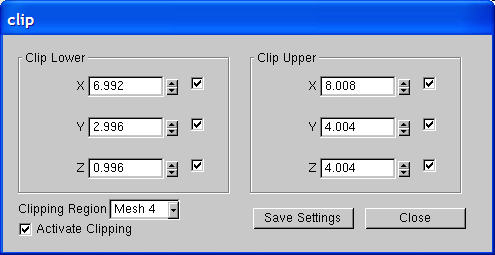
\includegraphics[width=4.2708333in]{FIGURES/figCLIP}
\end{center}
\caption[Clipping dialog box]{Clipping dialog box.  Clipping
entries result in the view shown in Figure \ref{figCLIPPED}b.
Clipping entries may be changed individually or selected by mesh
number. } \label{figCLIP}
\end{figure}

\begin{figure}[\figoptions]
\begin{center}
\begin{tabular}{cc}
\includegraphics[width=3.507in]{FIGURES/sprinkhall4a}&\includegraphics[width=3.507in]{FIGURES/sprinkhall4b}\\
a) full scene&b) scene clipped to mesh 4\\
\end{tabular}
\end{center}
\caption[Two views of a multi-mesh case.]{Two views of a
multi-mesh case. The first view shows the entire scene, the second
view shows the scene clipped to mesh 4. The clipping entries
producing the second view are shown in Figure \ref{figCLIP}.}
\label{figCLIPPED}
\end{figure}

It is difficult to view the interior of a scene when modelling
complicated geometries.  To alleviate this problem, portions of
the scene may be hidden or clipped by defining up to six clipping
planes. OpenGL draws the scene on one side of a clipping plane but
not the other. In general, a clipping plane may have any
orientation. Smokeview defines two clipping planes for each of the
three coordinate axes.   The two x axis clipping planes clip
regions with $x$ coordinates smaller than an `$x_{min}$' clipping
value and larger than an `$x_{max}$' value. The y axis and z axis
clipping planes behave similarly.  Clipping plane values are
specified using the clipping dialog box which is opened by
selecting the \frameit{Dialogs$>$Clip Geometry}\ menu item. Figure
\ref{figCLIP} shows this dialog box with all planes active and
values selected for mesh 4 of the scene.  The corresponding
clipped scene is illustrated in Figure \ref{figCLIPPED}.

\section{Setting Data Bounds}

Normally, \smokeview\ determines data bounds automatically
when it loads data. Sometimes, however, it is desirable to
override \smokeview's choice.  This allows for consistent
color shading when displaying several data files
simultaneously.

\begin{figure}[\figoptions]
\centerline{\includegraphics[width=1.993055in]{FIGURES/figBOUNDSplot3d}
} \caption[File/Bounds dialog box showing PLOT3D file options]
{File/Bounds dialog box showing PLOT3D file options. Select a
variable and a bounds type {\em check box/radio button}, then enter
a lower and/or upper bound. Data may be excluded from the plot by
selecting a {\em Truncate}\ bound.  Select type of contour plot to be
displayed. Press {\em Reload...}\ or {\em Update}\ for the new bounds to
take effect.} \label{figBOUNDSplot3d}
\end{figure}

The \fbox{\tt Set Bounds...} dialog box is opened from the
\frameit{Dialogs}\ menu. Each file type in Figure
\ref{figBOUNDSplot3d} (slice, particle, Plot3D \etc) has a set of
{\em radio buttons}\ for selecting the variable type that data bounds
are to be applied to. These variable types are determined from the
files generated by \fds\ and are automatically recorded in the
{\tt .smv} file. The data bounds are set in a pair of edit boxes.
Radio buttons adjacent to the edit boxes determine what type of
bounds should be applied.  The \frameit{Update}\ and
\frameit{Reload}\ buttons are pressed to make the new bounds take
effect.

\begin{figure}[\figoptions]
\centerline{\includegraphics[width=2.222222in]{FIGURES/figBOUND2}
} \caption[File/Bounds dialog box showing slice and boundary file
options] {File/Bounds dialog box showing slice and boundary file
options. Select a variable and a bounds type {\em check box/radio
button}, then enter a lower and/or upper bound. In the slice
portion, data may be excluded from the plot by selecting a
{\em Truncate}\ bound. In the boundary portion, ignited materials may
be highlighted if a wall temperature boundary file has been saved.
 Press {\em Reload...}\ or {\em Update}\ for the new bounds to take
effect.} \label{figBOUNDSslice}
\end{figure}

\begin{figure}[\figoptions]
\begin{center}
\begin{tabular}{ccc}
\includegraphics[height=\figheightAbar]{figures/thouse3d2_0025}&
\includegraphics[height=\figheightAbar]{figures/thouse3d2_0050}\\
5.0 s&10.0 s\\
\includegraphics[height=\figheightAbar]{figures/thouse3d2_0150}&
\includegraphics[height=\figheightAbar]{figures/thouse3d2_0300}&\\
30.0 s&60.0 s
&\raisebox{0.0ex}[0pt]{\includegraphics[height=5.0in]{figures/colorbar_20_620}}\\
\end{tabular}
\caption [Ceiling Jet Visualization.] {   Ceiling jet
visualization created by {\em chopping data}\ below 140~$^\circ$C
using the {\tt Bounds Dialog Box} as illustrated in
Figure~\ref{figBOUNDSslice}. }
\label{figceilingjet}%
\end{center}
\end{figure}

The {\tt Plot3D} and {\tt Slice File}\ portions of the bounds
dialog box have additional controls used to chop or hide data.
The settings used in Figure \ref{figBOUNDSslice} were used to
generate the ceiling jet visualized in Figure~\ref{figceilingjet}.
Data values less than 140\degC\ are chopped or not drawn in the
figure.

Slice file data may be time averaged or smoothed over a user
selectable time interval.  This option is also implemented from
the Slice File section of the bounds dialog box (see Figure
\ref{figBOUNDSslice}.

The {\bf Boundary File}\ portion of the dialog box has an {\bf
ignition} checkbox which allows one to visualize when and where
the blockage temperature exceeds its ignition temperature.

The bounds dialog for PLOT3D display allows one to select between
three different types of contour plots:  shaded, stepped and line
contours.

\section{3D Smoke Options}
\begin{figure}[\figoptions]
\centerline{\includegraphics[width=2.8264in]{FIGURES/fig3DSmoke} }
\caption[Dialog Box for setting 3D smoke options] {Dialog box for
setting 3D smoke options.   } \label{fig3DSmoke}
\end{figure}
Figure \ref{fig3DSmoke} allows one to override Smokeview's choice
for several of the 3D smoke parameters.  The user may specify the
color of the fire and the gray level of the smoke.  A gray level
of $n$ where n ranges from 0 to 7 results in a color of
$(2^n,2^n,2^n)$ where the three components represent red, green
and blue contributions.  The {\bf hrrpuv cutoff} input refers to
the heat release rate required at a node before Smokeview will
color the node as fire rather than smoke.  The {\bf 50\% flame
depth} allows one to specify the transparency or optical thickness
of the fire (for visualization purposes only). A small value
results in opaquely drawn fire while a large value results in a
transparently drawn fire. The {\bf Absorption Parameter} setting
refers to how the smoke slices are drawn.  The {\bf adjust
off-center} setting causes Smokeview to account for non-axis
aligned paths. The {\bf adjust off-center + zero at boundary}
accounts for off center path lengths and zeros smoke density at
boundaries in order to remove graphical artifacts.


\section{Plot3D Viewing Options} Plot3D files are more
complicated to visualize than time dependent files such as
particle, slice or boundary files. For example, only the
transparency and color characteristics of a time file may be
changed. With Plot3D files however, many attributes may be
changed. One may view 2D contours along the {\tt X}, {\tt Y}
and/or {\tt Z} axis of up to six\footnote{ The \fds\ software
stores temperature, three components of velocity (denoted $u$, $v$
and $w$) and heat release per unit volume.  If at least one
velocity component is stored in a Plot3D file, then \smokeview\
adds speed to the Plot3D variable list.} different simulated
quantities, view flow vectors and iso or 3D contours. Plot3D file
visualization is initiated by selecting the desired entry from the
\loadmenu\ {\tt Plot3D} sub-menu and as with time files one may
change color and transparency characteristics.

\paragraph{2D contours}
\Smokeview\ displays a 2D contour slice midway along the
{\tt Y} axis by default when a Plot3D file is first loaded,
To step the contour slice up by one grid cell along the
{\tt Y} axis, depress the {\em\tt space bar}. Similarly to
step the contour slice down by one grid cell along the {\tt
Y} axis, depress the ``{\tt -}'' key. To view a contour
along either the {\tt X} or {\tt Z} axis, depress the {\tt
x} or {\tt z} keys respectively.  Depressing the {\tt x},
{\tt y} or {\tt z} keys while the contour is visible will
cause it to be hidden. The Plot3D variable viewed may be
changed by either depressing the ``{\tt p}'' key or by
selecting the {\tt Solution Variable} sub-menu of the
\showmenu\ menu.

\paragraph{Iso-Contours}Iso-contours also called 3D contours or level surfaces may be
viewed by depressing the ``{\tt i} key or by selecting the
{\tt Plot3D 3D Contours} sub-menu of the \showmenu\ menu.

\paragraph{Flow vectors}If at least one velocity component is present in the Plot3D
file then the ``{\tt v}'' key may be depressed in order to
view flow  vectors. The length and direction of the vector
indicates the flow direction and speed. The vector color
indicates the value of the currently displayed quantity. A
small dot is drawn at the end of the line to indicate flow
direction. The vector lengths as drawn may be changed by
depressing the ``{\tt a}'' key. Vector plots may be very
dense when the grid is finely meshed. The ``{\tt s}'' key
may be depressed in order to skip vectors.  For example,
all vectors are displayed by default.  If the ``{\tt s}''
is depressed then every other vector is skipped.

\section{Display Options}
\subsection{General}
\begin{figure}[\figoptions]
\centerline{\includegraphics[width=5.13888in]{FIGURES/figProperties}
} \caption [Dialog Box for setting miscellaneous Smokeview scene
properties] {Dialog Box for setting miscellaneous Smokeview scene
properties} \label{figProperties}
\end{figure}
The display dialog box, illustrated in Figure \ref{figProperties},
allows one to set various options to control the display or
{\em look}\ of the Smokeview scene.  It may be invoked by selecting
the \frameit{Dialogs$>$Display} menu item.  This dialog box also
allows one to show or hide loaded data files.


\subsection{Stereo}
\begin{figure}[\figoptions]
\begin{center}
\includegraphics[height=2.0in]{figures/thouse5c_stereo}
\caption[Stereo pair view of a townhouse kitchen fire.]{
Stereo pair view of a townhouse kitchen fire. To aid in viewing the stereo effect, place
a finger in front of each image.  Relax your eyes allowing your two fingers and stereo pair
images to merge into one.
}
\label{figstereo}
\end{center}
\end{figure}

\begin{figure}[\figoptions]
\begin{center}
\includegraphics[height=1.5in]{figures/figSTEREO}
\caption{Dialog
box for activating the stereo view option.}
\label{figstereodialog}
\end{center}
\end{figure}
Smokeview implements two methods for displaying images in stereo or 3D.
Each method creates two versions of the scene, one version for each eye.
In one method, the two images are displayed alternately.  Specialized shuttered glasses are synched
with the monitor to ensure that the left eye sees only the left eye's version of the scene and that the right eye sees only the right eye's version  of the scene. To be effective the monitor requires a refresh rate of at least 120 frames per second (60 frames per second for each eye).
Flickering is annoyingly noticeable in monitors with slower frame rates.  Unfortunately, today's LCD flat panel monitors typically do not have refresh rates faster than 60 to 80 frames per second.  This method requires a video card that implements OpenGL {\em QUAD buffering}.
This Smokeview option can only be enabled from the command line by using the {\tt -stereo}\
option.

In the second method, Smokeview displays the two images side by side, again one image for each eye.  With practice, one can merge the images without requiring specialized equipment, especially if the images are small and not separated by a large angle.
A trick for seeing the stereo effect is to place a finger from each hand in the center of each picture.  Then relax your eyes, trying to {\em merge}\ your two fingers together.

Figure \ref{figstereo} shows
a pair of images of a townhouse kitchen fire.  Figure \ref{figstereodialog} shows the dialog
box used to activate this option.  If the {\em -stereo}\ command line option was used and
the video card supports shuttered stereo display then the {\em shuttered checkbox}\ in the dialog box will be enabled.

\section{Texture Maps} Texture mapping is a technique used by
Smokeview to make a scene appear more realistic by pasting images
onto obstructions or vents. For example, to apply a wood paneling
image to a wall, add the keywords {\tt
TEXTURE\_MAP='paneling.jpg', TEXTURE\_WIDTH=1., TEXTURE\_HEIGHT=2.
}\ to the {\tt \&SURF}\ line where {\bf paneling.jpg} is the JPEG
file containing the texture map (SGI users should use RGB files
instead of JPEG) and {\bf TEXTURE\_WIDTH}\ and {\bf
TEXTURE\_HEIGHT}\ are the characteristic dimensions of the texture
map in meters. Note that the image will not appear when Smokeview
first starts up. The user must select the texture maps using the
{\tt Show/Hide} menu.

One can create texture maps using a digital camera or obtain them
commercially.  The maps should be {\em seamless}\ so that no
breaks or seams appear when the maps are tiled on a blockage or
vent.  This is important, because Smokeview replicates the image
as often as necessary to cover the blockage or vent.

When the texture does have a pattern, for example windows or
bricks, the keyword {\tt TEXTURE\_ORIGIN} may be used to specify
where the pattern should begin.  For example,
\begin{verbatim}
&OBST XB=1.0,2.0,3.0,4.0,5.0,7.0,SURF_ID='wood paneling',
      TEXTURE_ORIGIN=1.0,3.0,5.0 /
\end{verbatim}
\noindent will apply paneling to an obstruction whose dimensions
are 1 m by 1 m by 2 m, such that the image of the paneling will be
positioned at the point (1.0,3.0,5.0). The default value of {\tt
TEXTURE\_ORIGIN} is (0,0,0), and the global default can be changed
by added a {\tt TEXTURE\_ORIGIN} statement to the {\tt MISC} line.

\begin{figure}[\figoptions]
\centerline{\includegraphics[width=4.8125in]{FIGURES/figTextures}
} \caption [Texture map example.] {
Texture map example.  The same texture was applied to two different
blockages and a vent (with different widths) by assigning different {\tt TEXTURE\_WIDTH}\
parameters in the input file.
} \label{figTextures}
\end{figure}
Figure \ref{figTextures} shows a simple application of a texture
applied to two different blockages and a vent.  The same jpeg file
was used in two different {\tt \&SURF}\ lines so that the texture
could be stretched by differing amounts (using the {\tt
TEXTURE\_WIDTH}\ parameter.)  The FDS data file used to create
this Figure follows.

\begin{verbatim}
&HEAD CHID='sillytexture',TITLE='Silly Test Case' /
&MISC TEXTURE_ORIGIN=0.1,0.1,0.1 /

&GRID IBAR=20,JBAR=20,KBAR=20 /
&PDIM XBAR=1.0,YBAR=1.0,ZBAR=1.0 /
&TIME TWFIN=0. /
&SURF ID     = 'TEXTURE 1'
      TEXTURE_MAP= 'nistleft.jpg'
      TEXTURE_WIDTH=0.6
      TEXTURE_HEIGHT=.20
      rgb=0.0,0.0,1.0
 /

&SURF ID     = 'TEXTURE 2'
      TEXTURE_MAP= 'nistleft.jpg'
      TEXTURE_WIDTH=0.4
      TEXTURE_HEIGHT=.20
      rgb=1.0,0.0,1.0
 /
&OBST XB=0.1,0.30, 0.1,0.7, 0.1,0.3, SURF_ID='TEXTURE 1'  /
&OBST XB=0.5,0.9, 0.3,0.7, 0.1,0.5 SURF_ID='TEXTURE 2'
      rgb=1.0,0.0,0.0 TEXTURE_ORIGIN=0.5,0.3,0.1  /

&VENT XB=0.00,0.00,0.2,0.8,0.20,0.40,SURF_ID='TEXTURE 1'
    rgb=0.0,1.0,0.0 TEXTURE_ORIGIN=0.0,0.2,0.2 /
&VENT XB=0.30,0.90,0.0,0.0,0.30,0.50,SURF_ID='TEXTURE 1'
    TEXTURE_ORIGIN=0.90,0.0,0.3 /
\end{verbatim}


\section{Using Smokeview to Debug FDS Input Files} One of the most difficult
tasks in setting up an \fds\ input file is defining the geometry
(blockages, vent locations \etc) properly. \Smokeview\ may be used
to debug \fds\ input files by making short runs and observing
whether blockages, vents and other geometric features of a run are
located correctly. Blockages may then be created or changed. This
is done with the {\em Edit Blockage}\ dialog box called from the
\fbox{\tt Option menu}.

The following is a general procedure for identifying problems in
\fds\ input files. Assume that the \fds\ input data file is named
{\tt testcase1.data}.
\begin{enumerate}
\item Set the stop time to $0.0$ using {\tt TWFIN=0.0} on the {\tt
\&TIME} line. This causes \fds\ to read the input file and create
a {\tt .smv} file without  performing lengthy startup
calculations.

\item After the input file has been modified, run the \fds\ model
(for details see the FDS User's Guide\cite{FDS_Users_Guide_4})

\noindent\ \FDS\ creates a file named {\tt testcase1.smv}
containing information that \smokeview\ uses to visualize data.
\item To visualize the input file, open {\tt testcase1.smv} with
\smokeview\ by either typing {\tt smokeview testcase1} at a
command shell prompt or if on the PC by double-clicking the file
{\tt testcase1.smv}.

\item Make corrections if necessary. Use the {\tt COLOR} or {\tt
RGB} option\footnote{The \fds\ {\tt COLOR} keyword may have
values: {\tt RED}, {\tt BLUE}, {\tt GREEN}, {\tt MAGENTA}, {\tt
CYAN}, {\tt YELLOW}, {\tt WHITE} or {\tt BLACK}. The {\tt RGB}
keyword uses three floating point inputs ranging from 0.0 to 1.0
to specify the red, green and blue components of color.  {\tt
COLOR} replaces {\tt BLOCK\_COLOR} and {\tt VENT\_COLOR}.} of the
{\tt OBST} keyword to more easily identify blockages to be edited.
For example, to change a blockage's color to red use:
\begin{verbatim}
&OBST XB=0.0,1.0,0.0,1.0,0.0,1.0 COLOR='RED' /
\end{verbatim}
\noindent or
\begin{verbatim}
&OBST XB=0.0,1.0,0.0,1.0,0.0,1.0 RGB=1.0,0.0,0.0 /
\end{verbatim}

\noindent Save testcase1.data file and go back to step 2.

\item If corrections are unnecessary, then change the {\tt TWFIN}
keyword back to the desired final simulation time, remove any
unnecessary \fds\ {\tt COLOR} keywords and run the case.
\end{enumerate}

\paragraph{Examining and/or Editing Blockages}  Blockages may be examined or changed by selecting
the menu item \frameit{Dialogs/Edit Geometry}\\ which opens up the dialog box
illustrated in Figure \ref{figEDIT}. Text edit boxes allow one to
define comments (any text to the right of the closing ``/'' on an
\&OBST line and pull down menus for linking surfaces (\&SURF
lines) to obstructions. The surface choices are obtained from the
input file or the database file if one is specified in the input
file.

Note, the blockage editor does not work when clipping planes are
active.

The user may associate one, three or six surfaces with an obstruction.
If the {\em\tt 3 wall} radio button is selected then materials
for the ceiling (upper surface), walls (vertical surfaces) and
floor (lower surface) may be specified. The {\tt\em color}\ check
box allows the inputted or default color (manilla) to be displayed
on blockage surfaces.

Associating unique colors with each surface allows the user to quickly
determine whether blockages are defined with the proper surfaces.
One can then verify that these modelling elements have been
defined and positioned as intended.

\begin{figure}[\figoptions]
\centerline{
\centerline{\includegraphics[width=4.826in]{FIGURES/figEDIT} } }
\caption[Blockage Edit Dialog Box] {Blockage Edit Dialog Box.
Click on `New' to create a new blockage or click on an existing
blockage in the Smokeview scene to change its size or location.
Change the size or location by entering blockage bounds directly
or clicking an `arrow' and/or direction buttons.  Note, the
blockage editor does not work when clipping planes are active.}
 \label{figEDITBLOCKS}
\label{figEDIT}
\end{figure}

The blockage editor works on one mesh at a time. For multi-mesh
cases, use the Mesh list-box to select the desired mesh or simply
click on a blockage in the mesh to switch to that mesh. The
pull-down menu is necessary for meshes without blockages.

Position coordinates entered into the text boxes are
{\em snapped}\ to the nearest grid line.  Materials appearing
under {\em\tt Surface Type}\ come from those materials
defined in either the input data file or the database file.
Either one, three or six wall properties can be entered by
selecting the appropriate radio button.

\section{Making Movies} \label{section:movie} A movie can be made
of a Smokeview animation by converting the visualized scene into a
series of PNG or JPEG files, one file for each time step and then
combining the individual images together into one movie file. More
specifically:

\begin{enumerate}
\item Set up Smokeview by orienting the scene and loading the
desired data files.

\item Select the \frameit{Options/Render} menu and pick the
desired frame skip value. The more frames you include in
the animation, the smoother it will look. Of course more
frames result in larger file sizes.  Choose fewer frames
if the movie is to appear on a web site.

\item Use a program such as the Antechinus Media Editor
available at \hhref{http://www.c-point.com} to assemble the
JPEGS or PNGS rendered in the previous step into a movie
file.
\end{enumerate}

The default Smokeview image size is $640\times 480$ .  This size
is fine if the movie is to appear in a presentation located on a
local hard disk.  If the movie is to be placed on a web site then
care needs to be taken to insure that the generated movie file is
a reasonable size.  Two suggestions are to reduce the image size
to $320\times 240$ or smaller by modifying the {\tt WINDOWWIDTH}
and {\tt WINDOWHEIGHT} smokeview.ini keywords  and to reduce the
number of frames to 300 or less by skipping intermediate frames
{\em via} the \frameit{Options/Render} menu.

Sometimes when copying or {\em capturing}\ a Smokeview scene it is
desirable, or even necessary, to have a margin around the scene.
This is because the capturing system does not include the entire
scene but itself captures an indented portion of the scene. To
indent the scene, either press the ``h'' key or select the
\frameit{Option$>$Viewpoint$>$Offset Window}\ menu item. The
default indentation is 45 pixels. This may be changed by
adding/editing the WINDOW\_OFFSET keyword in the smokeview.ini
file.

\section{Annotating the Scene }
\label{section:annotate} \label{subsect_features} Smokeview
rendered JPEG or PNG image files may be annotated with any package
that edits these types of files. Tick marks and label annotation
can be placed within the 3D scene and moved around as the scene is
moved. This would be difficult to duplicate with an external image
editor. In addition, axis labels are displayed, if desired, by
selecting \showmenu $>$\fbox{\tt Labels}$>$\fbox{\tt Axis labels}.


The current release of FDS places tick marks and labels
documenting the scene dimensions.  To replace or customize
these annotations add the {\tt TICK} keyword to a .smv file
using the following format:

\begin{verbatim}
TICKS
xb yb zb xe ye ze nticks
ticklength tickdir r g b tickwidth
\end{verbatim}

\noindent where {\tt xb}, {\tt yb}, and {\tt zb} are the x, y and
z coordinates of the first tick; {\tt xe}, {\tt ye} and {\tt ze}
are the x, y and z coordinates of the last tick and {\tt nticks}
is the number of ticks. The coordinate dimensions are in physical
units, the same units used to set up the FDS geometry. The
parameter {\tt ticklength} specifies the lengh of the tick in
physical units. The parameter {\tt tickdir} specifies the tick
direction.  For example 1(-1) places ticks in the
positive(negative) x direction. Similarly, 2(-2) and 3(-3) place
ticks in the positive(negative) y and positive(negative) z
directions.

The color parameters {\tt r}, {\tt g} and {\tt b} are the
red, green and blue components of the tick color each
ranging from 0.0 to 1.0. The foreground color (white by
default) may be set by setting any or all of the {\tt r},
{\tt g} and {\tt b} components to a negative number. The
{\tt tickwidth} parameter specifies tick width in pixels.
Fractional widths may be specified.

The {\tt LABEL} keyword allows a text string to be added
within a Smokeview scene.  The label color and start and
stop appearance time may also be specified. The format is
given by

\begin{verbatim}
LABELS
x y z r g b tstart tstop
label
\end{verbatim}

\noindent where ({\tt x, y, z}) is the label location in cartesian
coordinates and {\tt r, g, b} are the red, green and blue color
components ranging from 0.0 to 1.0.  Again, if a negative value is
specified then the foreground color will be used instead (white is
the default).  The parameters, {\tt tstart} and {\tt tstop}
indicate the time interval when the label is visible. The text
string is specified on the next line ({\tt label}).

\begin{figure}[\figoptions]
\begin{center}
\includegraphics[height=3.0in]{figures/ticklabels}
\end{center}
\caption{ Annotation example using the TICKS and LABEL keword. }
\label{figticklabels}%
\end{figure}
Figure \ref{figticklabels} shows how the {\tt LABEL} and
{\tt TICKS} keywords can be used together to create a
{\em ruler}\ with major and minor tick marks.  These ticks and
labels were created using:

{\small
\begin{verbatim}
TICKS
0.0 0.0 0.0 8.0 0.0 0.0 5
0.5 -2.0 -1. -1.0 -1.0 4.0
TICKS
1.0 0.0 0.0 9.0 0.0 0.0 5
0.25 -2.0 -1. -1.0 -1.0 4.0
TICKS
0.0 0.0 0.0 0.0 0.0 2.0 3
0.5 -1.0 -1. -1.0 -1.0 4.0
TICKS
0.0 0.0 0.0 0.0 4.0 0.0 5
0.5 -1.0 -1. -1.0 -1.0 4.0
LABEL
0.0 -0.6 0.0 -1.0 0.0 0.0 0.0 20.0
0
LABEL
2.0 -0.6 0.0 -1.0 0.0 0.0 0.0 20.0
2
LABEL
4.0 -0.6 0.0 -1.0 0.0 0.0 0.0 20.0
4
LABEL
6.0 -0.6 0.0 -1.0 0.0 0.0 0.0 20.0
6
LABEL
8.0 -0.6 0.0 -1.0 0.0 0.0 0.0 20.0
8
LABEL
9.5 -0.6 0.0 -1.0 0.0 0.0 0.0 20.0
m
\end{verbatim}
}

\section{Creating Custom Devices}
Smokeview draws devices such as heat and smoke detectors,
sprinklers, sensors {\em etc.} using instructions contained in a
data file.  These instructions correspond to OpenGL library calls,
the same type of calls Smokeview uses to visualize FDS cases.
Smokeview then acts as an OpenGL interpreter executing OpenGL
commands as specified in the device definition file. Efficiency is
obtained by compiling these instructions into display lists,
terminology for an OpenGL construct for storing and efficiently
drawing collections of OpenGL {\em commands}.

This section describes how to create new devices. Though all of
the examples are given for devices, the intent of this procedure
is to be more general allowing Smokeview to draw other types of
objects such as people walking.

There are two types of instructions, instructions for drawing
simple geometric objects such as cubes, disks, spheres {\em etc.}
and instructions for manipulating these objects through scaling,
rotation and translation. Collectively these instructions specify
the type, location and orientation of objects used to represent
devices.  The important feature of this process is that new
devices may be designed and drawn without the need to modify
Smokeview.

\subsection{Device File Format}
The format for an object definition file is given in Figure
\ref{figobjectdef}.  Each device definition consists of one or two
frames.  Devices such as thermocouples which do not activate use
just one frame. Other devices such as sprinklers or smoke
detectors which do activate use two frames, the first for normal
conditions and the second for when the device has activated.

\begin{figure}[\figoptions]
{\small
\begin{Verbatim}[frame=single,rulecolor=\color{blue},
framerule=3pt,framesep=1pc,fillcolor=\color{yellow}]
DEVICEDEF
   //  comments follow the double slash

   //  blank lines ^^^^^^ are permitted
   //  any line not begging with a double "slash"
   //   is part of the devices definition.
  device_name // name or type of device
  // comments and blank lines

  // are permitted anywhere
  args command1 args command2 ...  // arguments followed by command name
  args command1 args command2 ...  // arguments and commands may be split
                                   // across lines
 NEWFRAME    // beginning of next frame
  args command args command  ...
  ....
\end{Verbatim}
} \caption{Device Object file format}
\label{figobjectdef}%
\end{figure}

Each definition begins with the {\tt DEVICEDEF}\ keyword.  The
next non-comment line contains a label naming the device.
Succeeding lines contain one or more commands, each pre-pended by
zero or more numerical arguments.   New frames begin with the {\tt
NEWFRAME}\ keyword.  Blank lines may occur anywhere.  Definitions
may be documented by adding comments following the {\tt `//'}\
characters.

Some examples of command/argument pairs are {\tt d drawsphere} for
drawing a sphere of diameter {\tt d} or {\tt x y z translate} for
translating an object by $(x,y,z)$. Transformation commands are
cumulative, each command builds on the effects of the previous
command.  The {\tt push}\ and {\tt pop}\ then may be used to
isolate these effects by saving and restoring the geometric state.
More details may be found in the next two sections.

A simple example of a definition used to draw a sensor along with
the corresponding Smokeview view is given in Figure
\ref{figsensor}. The definition uses just one frame. A sphere is
drawn with color yellow and diameter 0.38 m. Push and pop commands
are not necessary because there is only one object and no
transformations are used.

Figure \ref{figsprinkler} is more complicated. It shows a
definition for an up-right sprinkler along with a corresponding
Smokeview view. The definition uses two frames. The first frame
represents the sprinkler's inactive state, the second frame
represents the active state (commands after the {\tt NEWFRAME}\
keyword). This definition uses cubes, a truncated cone, spheres,
disks and a notched plate. The cube is stretched and rotated using
the scale and rotate commands forming the two sloped `bars'. The
other parts are moved into their proper position using the
translate command. The push and pop commands are used to isolate
the effects of transformation commands for one part when drawing
another.

\begin{figure}[\figoptions]
\begin{Verbatim}[frame=single,rulecolor=\color{blue},
framerule=3pt,framesep=1pc,fillcolor=\color{yellow}]
DEVICEDEF
 sensor
 1.0 1.0 0.0  setcolor
 0.038 drawsphere
\end{Verbatim}
\begin{center}
\includegraphics[height=\figheightA]{figures/sensorplain}\\
\end{center}
\caption{Instructions for drawing a sensor along with the corresponding Smokeview view.}
\label{figsensor}%
\end{figure}

\begin{figure}[\figoptions]
{\bf Heat detector Instructions}\\
{\small
\begin{Verbatim}[frame=single,rulecolor=\color{blue},
framerule=3pt,framesep=1pc,fillcolor=\color{yellow}]
DEVICEDEF
 heat_detector         // label, name of device

 // The heat detector has three parts
 //   a disk, a truncated disk and a sphere.
 //   The sphere changes color when activated.

 0.8 0.8 0.8 setcolor  // set color to off white
 push 0.0 0.0 -0.02 translate 0.127 0.04 drawdisk pop
 push 0.0 0.0 -0.04 translate 0.06 0.08 0.02 drawtrunccone pop
 0.0 1.0 0.0 setcolor
 push 0.0 0.0 -0.03 translate  0.04 drawsphere pop
 // push and pop are not necessary in the last line
 //   of a frame.  Its a good idea though, to prevent
 //   problems if parts are added later.
NEWFRAME  // beginning of activated definition
 0.8 0.8 0.8 setcolor
 push 0.0 0.0 -0.02 translate 0.127 0.04 drawdisk pop
 push 0.0 0.0 -0.04 translate 0.06 0.08 0.02 drawtrunccone pop
 1.0 0.0 0.0 setcolor
 push 0.0 0.0 -0.03 translate 0.04 drawsphere pop
\end{Verbatim}
}
\begin{center}
\begin{tabular}{cc}
 \includegraphics[height=\figheightA]{figures/heatdetector_inact}&
 \includegraphics[height=\figheightA]{figures/heatdetector_act}\\
inactive&active\\
 \end{tabular}
 \end{center}
\caption{Instructions for drawing an inactive and active heat detector
along with the corresponding Smokeview view }
\label{figsprinkler}%
\end{figure}


\newcommand{\devfig}[1]{
\includegraphics[height=1.7in]{figures/#1}
}

As with preference ({\tt .ini}) files, Smokeview looks for device
definitions in three places.  First, in a file named {\tt
devices.svo}, in the directory containing the Smokeview program.
On the PC, this is {\tt
C:$\backslash$nist$\backslash$fds$\backslash$} . Next, in a file
named {\tt devices.svo}, in the directory containing the case
being viewed and finally in a file named {\tt casename.svo} where
{\tt casename} is thet name of the case.

The global file, {\tt devices.svo}, contains definitions for a
sprinkler (upright and pendent), heat detector, smoke detector,
sensor and nozzle.  Figure \ref{figdevicesr} gives Smokeview views
for theses devices.  Active views are shown when they are defined.
The object's origin is identified by the three intersecting lines.
The origin is placed where FDS records data for these devices.

\begin{figure}[\figoptions]
\begin{center}
\begin{tabular}{ccc}
 \devfig{sprinkler_inact}&\devfig{pendent_inact}&\devfig{nozzle_inact}\\
 inactive up-right sprinkler&inactive pendent sprinkler&inactive nozzle\\
 \devfig{sprinkler_act}  &\devfig{pendent_act}  &\devfig{nozzle_act}\\
 active up-right sprinkler&active pendent sprinkler&active nozzle\\
 \devfig{smokedetector_inact}&\devfig{heatdetector_inact}&\devfig{target}\\
 inactive smoke detector&inactive heat detector&target\\
 \devfig{smokedetector_act}  &\devfig{heatdetector_act}  &\devfig{sensor}\\
 active smoke detector&active heat detector&sensor
 \end{tabular}
 \end{center}
\caption[Smokeview view of devices defined in the global
devices.svo file] {Smokeview view of devices defined in the global
devices.svo file.  The device origin occurs at the intersection of
the thin (green) lines, where data is recorded in FDS.}
\label{figdevicesr}%
\end{figure}

\subsection{Geometric Objects}
\label{svocommands} Each command used to draw elementary geometric
objects consists of one or more arguments followed by the command
{\em e.g.}\ {\tt 0.3 drawsphere}. Some portion of the object is
designated as the origin, {\em i.e.}\ with coordinate $(0,0,0)$.
The location of the origin is needed when assembling geometric
objects together to form more complex objects.  The transformation
commands discussed in the next section are used to perform this
assembly, specifying exactly where and with what orientation the
geometric objects should be placed.


\newcommand{\infigr}[2]{
\parpic[r]{
\begin{tabular}{c}
\includegraphics[height=\infigheight]{figures/#1}\\
{\tiny\tt #2}
\end{tabular}
}
}
\newcommand{\infigl}[2]{
\parpic[l]{
\begin{tabular}{c}
\includegraphics[height=\infigheight]{figures/#1}\\
{\tiny\tt #2}
\end{tabular}
}
}
%\infigr{circle}{0.5 drawcircle}
\paragraph{DRAWCIRCLE} The command, {\tt d drawcircle },
draws a circle with diameter d.  The origin is located at the center of the circle.

\infigr{cone}{0.50 0.30 drawcone}
\paragraph{DRAWCONE}
The command, {\tt d h drawcone}, draws a right circular cone where
d is the diameter of the base and h is the height. The origin is
located at the center of the cone's base.

\infigl{cube}{0.25 drawcube}
\paragraph{DRAWCUBE} The command, {\tt s drawcube},
draws a cube where s is the length of the side.  The origin is
located at the center of the cube.  An oblong box, a box with
different length sides, may be drawn by using {\tt scale}\ along
with {\tt drawcube}.  For example, {\tt 1.0 2.0 4.0 scale 1.0
drawcube}\ creates a box with dimensions $1\times 2\times 4$.

\infigr{disk}{0.25 0.50 drawdisk}
\paragraph{DRAWDISK} The command, {\tt d h drawdisk},
draws a circular disk with diameter d and height h. The origin is
located at the center of the disk's base.\vspace{0.25in}

\infigl{hexdisk}{0.5 0.25 drawhexdisk}
\paragraph{DRAWHEXDISK} The command, {\tt d h drawhexdisk},
draws a hexagonal disk with diameter d and height h.  The origin
is located at the center of the hexagon's base.

%\infigr{line}{0.0 0.0 -0.5 0.0 0.0 0.5}
\paragraph{DRAWLINE} The
command, {\tt x1 y1 z1 x2 y2 z2 drawline}, draws a line between
the points $(x_1,y_1,z_1)$ and $(x_2,y_2,z_2)$.\vspace{0.25in}

\parpic[r]{
\begin{tabular}{cc}
\includegraphics[height=\infigheight]{figures/notchplate}&
\includegraphics[height=\infigheight]{figures/pendent}\\
{\tiny\tt  0.5 0.1 0.2 1 drawnotchplate}&
{\tiny\tt 0.5 0.1 0.2 -1 drawnotchplate}
\end{tabular}
}
\paragraph{DRAWNOTCHPLATE} The command, {\tt d h nh dir drawnotchplate},
draws a  notched plate.  This object is used to represent a
portion of a sprinkler where d is the plate diameter, h is the
plate height (not including notches), nh is the height of the
notches and dir indicates the notch orientation (1 for vertical,
-1 for horizontal).  The origin is located at the center of the
plate's base.

\paragraph{DRAWPOINT} The command, {\tt drawpoint}, draws a point
(small square).  The command, {\tt s setpointsize}\ may be used to
change the size of the point.  The default size is 1.0 .

\infigl{polydisk}{5 0.35 0.15 drawpolydisk}
\paragraph{DRAWPOLYDISK} The command, {\tt n d h drawpolydisk},
draws an n-sided polygonal disk with diameter d and height h.  The
origin is located at the center of the polygonal disk's base.  The
example to the left is a pentagonal disk.

\infigr{ring}{0.3 0.5 0.1 drawring}
\paragraph{DRAWRING} The command, {\tt di do h drawring},
draws a ring where {\tt di}\ and {\tt do}\ are the inner and outer
ring diameters and h is the height of the ring. The origin is
located at the center of the ring's base.

\infigl{sphere}{0.25 drawsphere}
\paragraph{DRAWSPHERE} The command, {\tt d drawsphere},
draws a sphere with diameter d.  The origin is located at the
center of the sphere. As with an oblong box, an ellipsoid may be
drawn by using {\tt scale}\ along with {\tt drawsphere}. For
example, {\tt 1.0 2.0 4.0 scale 1.0 drawsphere}\ creates an
ellipsoid with semi-major axes of length 1, 2 and 4. This is how
the sprinkler {\em bulb}\ in Figure \ref{figsprinkler}a is drawn.

\infigr{truncatedcone}{0.5 0.2 0.4 drawtrunccone}
\paragraph{DRAWTRUNCCONE} The command, {\tt d1 d2 h drawtrunccone},
draws a right circular truncated cone where d1 is the diameter of
the base, d2 is the diameter of the truncated portion of the cone
and h is the height or distance between the lower and upper
portions of the truncated cone.  The origin is located at the
center of the truncated cone's base.

\subsection{Transformations}
As with geometric commands, transformation commands consist of one
or more arguments followed by the command (except for {\tt push}
and {\tt pop}\ which do not require any arguments). Transformation
commands are used to change the location and orientation of drawn
objects, to save and restore the geometric state and to set
attributes such as point size, line width or object color. The
rotate and translate commands change the origin (translate) or
orientation of the x,y,z axes (rotate). The PUSH command is then
used to save the origin or axis orientation while the POP command
is used to restore the origin and axis orientation.

\blist

\hitem{POP} The command, {\tt pop}, restores the origin and axis
orientation saved using a previous {\tt pop}\ command.  The total
number of {\tt pop}\ and {\tt push}\ commands must be equal,
otherwise a fatal error would occur.  Smokeview detects this
problem and draws a red sphere instead of the errantly defined
object.

\hitem{PUSH} The command, {\tt push}, saves the origin and axis
orientation. (see above comment about number of {\tt push}\ and
{\tt pop}\ commands).

\hitem{ROTATEX} The command, {\tt r rotatex}, rotates objects
drawn afterwards {\tt r} degrees about the x axis.

\hitem{ROTATEY} The command, {\tt r rotatey}, rotates objects
drawn afterwards {\tt r} degrees about the y axis.

\hitem{ROTATEZ} The command, {\tt r rotatez}, rotates objects
drawn afterwards {\tt r} degrees about the z axis.  A cone or any
object for that matter may be drawn upside down by adding a {\tt
rotatez}\ command as in {\tt 180 rotatez 1.0 0.5 drawcone}.

\hitem{SCALEXYZ} The command, {\tt x y z scalexyz}, stretches
objects drawn afterwards by x, y and z respectively along the x, y
and z axes. The {\tt scalexyz}\ along with the {\tt drawsphere}\
commands would be used to draw an ellipsoid by stretching a sphere
along one of the axes.

\hitem{SCALE} The command, {\tt xyz scale}, stretches objects
drawn afterwards xyz along each of the x, y and z axes (equivalent
to {\tt xyz xyz xyz scalexyz} ).

\hitem{SETBW} The command, {\tt grey setbw}, sets the red, green
and blue components of color to grey (equivalent to grey grey grey
setcolor ).  As with the {\tt setcolor}\ command, {\tt setbw}\ is
only required when the grey level changes, not for each object
drawn.

\hitem{SETCOLOR} The command, {\tt r g b setcolor}, sets the red,
green and blue components of the current color.  Any object's
drawn afterwards will be drawn with this color.  That is, a {\tt
setcolor}\ command is not required for each object part drawn.

\hitem{SETLINEWIDTH} The command, {\tt w setlinewidth}\, sets the
width of lines drawn with the {\tt drawline}\ and {\tt
drawcircle}\ commands.

\hitem{SETPOINTSIZE} The command, {\tt s setpointsize}, sets the
size of points drawn with the {\tt drawpoint}\ command.

\hitem{TRANSLATE} The command, {\tt x y z translate}, translates
objects drawn afterwards by x, y and z along the x, y and z axes
respectively.  Equivalently, one can think of think of {\tt x y z
translate}\ as translating the origin by (-x,-y,-z).

\elist


\section{Smokezip - Compressing 3D Smoke and Boundary Files}

\begin{figure}[\figoptions]
\centerline{\includegraphics[width=1.6666in]{FIGURES/figBOUND1} }
\caption[Compression and Autoload dialog box] {File/Bounds dialog
box showing compression and autoload options.  3D smoke boundary
files may be compressed using smokezip.  All currently loaded
files may be loaded automatically when smokeview first starts by
selecting the autoload checkbox.} \label{figBOUNDScompress}
\end{figure}

3D smoke and boundary files may now be compressed using the
stand-alone program smokezip or from within Smokeview using the
compression menu item found on the Load/Unload menu.  File
compression may also be activated from the Compressions, Autoload
section of the File Bounds dialog box illustrated in Figure
\ref{figBOUNDScompress}. Compression is performed using the ZLIB
compression library (see \hhref{http://www.zlib.org} ). When using
Smokeview, compression is performed in the {\em background}\
allowing one to continue visualization.  Smokeview adds the label
{\em ZLIB}\ to Load menu entries for any files that have been
compressed. Smokezip adds the extension svz to the corresponding
compressed file name.

The usage for Smokezip is
\begin{verbatim}
smokezip 1.0 - Mar 12 2006

  Compresses Smokeview 3D smoke and boundary files

  smokezip [-f] [-s sourcedir] [-d destdir] [-c] casename [destdir]
\end{verbatim}

\blist
\hitem{-f} - overwrites compressed boundary and 3d smoke files
\hitem{-d destdir} - if specified will copy compressed files (and files needed
by Smokeview to view the case) to the directory destdir
\hitem{-s sourcedir} - if specified assumes all files are in
directory sourcedir
\hitem{-c}  - clean or remove all compressed files
\hitem{casename} - Smokeview .smv file
\elist

Smokezip uses min and max specifications found in the casename.ini
file to determine how to map the four byte floating point data
found in the boundary files to one byte color indices used by
Smokeview. Smokezip uses percentile min and max bounds if the
casename.ini file does not exist. The algorithms for determining
the data mappings used by Smokeview and Smokezip are identical so
should result in the same views.

%---------------------------------------------------------------------------------
%------------------------ Summary ------------------------------------------------
%---------------------------------------------------------------------------------

\chapter{Summary}
Often fire modeling is looked upon with skepticism because of the
perception that eye-catching images shroud the underlying physics.
However, if the visualization is done well, it can be used to
assess the quality of the simulation technique. The user of FDS
chooses a numerical grid on which to discretize the governing
equations. The more grid cells, the better but more time-consuming
the simulation. The payoff for investing in faster computers and
running bigger calculations is the proportional gain in realism
manifested by the images. There is no better way to demonstrate
the quality of the calculation than by showing the realistic
behavior of the fire.

Up to now, most visualization techniques have provided useful ways
of analyzing the output of a calculation, like contour and
streamline plots, without much concern for realism. A
rainbow-colored contour map slicing down through the middle of a
room is fine for researchers, but for those who are only
accustomed to looking at real smoke-filled rooms, it may not have
as much meaning. Good visualization needs to provide as much
information as the rainbow contour map but in a way that speaks to
modelers and non-modelers alike. A good example is smoke
visibility. Unlike temperature or species concentration, smoke
visibility is not a local quantity but rather depends on the
viewpoint of the eye and the depth of field. Advanced simulators
and games create the illusion of smoke or fog in ways that are not
unlike the techniques employed by fire models to handle thermal
radiation. The visualization of smoke and fire by Smokeview is an
example of the graphics hardware and software actually computing
results rather than just drawing pretty pictures. A common concern
in the design of smoke control systems is whether or not building
occupants will be able to see exit signs at various stages of a
fire. FDS can predict the amount of soot is located at any given
point, but that doesn't answer the question. The harder task is to
compute on the fly within the visualization program what the
occupant would see and not see. In this sense, Smokeview is not
merely a {\em post-processor}, but rather an integral part of the
analysis.




\bibliography{../refs/math,../refs/forney,../refs/fire,../refs/graphics}
\addcontentsline{toc}{chapter}{References}

\appendix
\addcontentsline{toc}{chapter}{Appendices}

%---------------------------------------------------------------------------------
%------------------------ Command Line Options -----------------------------------
%---------------------------------------------------------------------------------

\chapter{Command Line Options}
\label{sectioncommand} \Smokeview\ may be run from a command
shell.  Furthermore, command line options may be invoked in order
to alter \smokeview's startup behavior. Normally these options are
not necessary.  However, they may be used for cases with very
large particle files or to generate a preference or customization
file. To obtain a list of command line options, type:
\begin{verbatim}
smokeview -help
\end{verbatim}
\noindent without any arguments which results in output similar to:\\

\begin{verbatim}
Smokeview 5.0.0 Beta - May  6 2007
Visualize fire/smoke flow simulations.  All parameters are optional.

Usage:

smokeview casename -points m -frames n -ini -part -nopart -stereo -build

where

  casename = project id (file names without the extension)
         m = maximum number of particles.  Default=50000000
         n = maximum number of particle frames.  Default=5001
      -ini = output default smokeview parameters to smokeview.ini
     -part = load particle file if present
   -nopart = do not load particle file
   -stereo = activate stereo mode (if supported)
    -build = show pre-preprocessing directives used to build smokeview
\end{verbatim}

\noindent The {\tt -nopart} option is used to prevent a particle
file from being loaded at startup. The {\tt -points} and {\tt
-frames} options are used to load more than the default 5,000,000
points or 500 frames where a frame is data for one time step. To
load up to 6,000,000 points and 1000 frames then type:
\begin{verbatim}
smokeview casename -points 6000000 -frames 1000
\end{verbatim}
\noindent where in both cases {\tt casename} is the basename of
the \fds\ output files. The same effect may be achieved by using:
\begin{verbatim}
MAXPOINTS
6000000
MAXFRAMES
1000
\end{verbatim}
\noindent in the {\tt smokeview.ini} or {\tt casename.ini} file.
This file may be created with the {\tt -ini} option and contains
many other customizable \smokeview\ parameters. The {\tt
-benchmark} option is used to measure the performance of
\smokeview. The {\tt -benchmark} option causes \smokeview\ to
produce precise timings by outputting frame rates based upon one
cycle through the timing loop rather than using moving averages.
The {\tt -stereo} option may used to access stereo hardware (often
called quad buffering) if it is available.

%---------------------------------------------------------------------------------
%------------------------ Menu Options -------------------------------------------
%---------------------------------------------------------------------------------

\chapter{Menu Options}
\label{sectionmenu}
% --------------------MENU OPTIONS -----------------------

The design philosophy used to develop \smokeview\ has been
to avoid complicated, non-portable user interfaces that are
costly to implement.  As a result, most of the development
effort has gone into the visualization (display of particle
flow, contour plots \etc) rather than user interface design
and implementation. Smokeview's pop-up menus are
implemented with GLUT\cite{OpenGLGlut}, the graphics
library utility toolkit. The user interacts with
\smokeview\ \via 1) menus, 2) keyboard shortcuts and 3) the
preference file ({\tt smokeview.ini} or {\tt
casename.ini}).

A {\em pop up}\ menu is displayed when the right mouse is clicked
anywhere within the scene.  The main menu options as illustrated
in Figure \ref{fig_mainmenu} are: \loadmenu\, \showmenu,
\frameit{Options}, \frameit{Dialogs}\, \frameit{Tours},
\frameit{View}, \frameit{Help} and \frameit{Quit}. Several of
these menu options have sub-menus. These menus are described in
the following sections.

\section{Main Menu Items}

\begin{figure}[\figoptions]
\begin{center}
\includegraphics[width=1.513888in]{figures/menu_main2}
\caption{Main Menu} \label{fig_mainmenu}
\end{center}
\end{figure}

\blist

\hitem{Load/Unload}This menu option allows one to load or unload
particle, isosurface, vector slice, slice, Plot3D or boundary
files. These time dependent files may be viewed simultaneously,
but not concurrently with the time independent Plot3D files.
However, one boundary or one Plot3D file per mesh may be viewed at
a time. Multiple slices for the same variable may be viewed
simultaneously. This menu may also be used to load and create
preference files {\tt .ini files} and to re-read the {\tt .smv}
file. For more details see Appendix \ref{sectload}.
\\

\hitem{Show/Hide}This menu item allows one to show or hide
the loaded data files and various scene attributes such as
time/color bars, internal blockages \etc. As a file type is
shown or hidden (or loaded and unloaded), the color and
time bars are changed to reflect the currently visible data
files.
More details are given in Appendix \ref{sectshow}.\\

\hitem{Options}This menu allows one to specify various
smokeview options such as specifying frame rates, dumping
the screen to a PNG or JPEG file, changing font sizes,
selecting dialog boxes \etc.

\hitem{Dialogs}This menu allows one to open/close various dialog
boxes for setting data bounds, controlling {\em look}\ of the 3D
smoke, specifying clip planes \etc.

\hitem{Tour}This menu displays a list of tours stored in the {\tt
casename.ini}\ preference file.  The {\tt manual}\ tour gives
control back to the user.  Tours may be defined using the Tour
dialog box.

\hitem{View}Resets the simulation scene to an alternate view. The
three choices are 1) exterior view, 2) interior view or a 3) user
defined view.  A viewpoint may be saved by using this menu or by
using the \fbox{\tt Viewpoint} sub-menu of the \frameit{Options}\
menu. If a time file is visible then two sub-menus occur allowing
one to reset the view back to the
original position or the time bar back to the initial time.\\

\hitem{Help}Displays a list and explanation of keyboard equivalent commands. \\

\hitem{Quit}Quit Smokeview.

\elist


\section{Load/Unload}
\begin{figure}[\figoptions]
\begin{center}
\includegraphics[width=3.25in]{figures/menu_load2}
\caption{Load/Unload Menu}
\label{fig_loadmenu}
\end{center}
\end{figure}

\label{sectload}Six types of files may be visualized with
\smokeview. These files are loaded using the \fbox{\tt
LOAD/UNLOAD} menus as illustrated in Figure
\ref{fig_loadmenu}. They are particle, vector slice, slice,
boundary, isosurface and Plot3D files. Note that vector
slice animations use two or more slice files to display the
animated vector slices. The format of the data contained in
these files is described in Appendix \ref{sectionfile}. A
sub-menu is present under \loadmenu\ for each file type
generated for the simulation. Selecting one of the files
appearing in the sub-menu causes it to be loaded and then
displayed. The data may be unloaded or freed by selecting
an \fbox{\tt Unload} menu item appearing under the file
list. Selecting \fbox{\tt Unload All}  as expected will
unload all files. To hide a data file, select the
\showmenu\ menu option corresponding to the  file type to
be hidden.

The \smokeview\ {\tt .smv} file contains information about
all data files appearing in the \loadmenu\  menu item. The
\fds\ field modelling software creates this file. (See
Appendix \ref{sectionsmv} for documentation on the format
of this file).

The character ``{\tt *}'' occurring before a file name in
one of the sub-menus indicates that the file has already
been loaded. If the file below is loaded but not visible,
then use the appropriate \showmenu\ option to make it
visible.

\blist

\hitem{Open Smokeview ({\tt .smv})}This menu item allows one (on
the PC) to use an open file dialog box to open a Smokeview scene
(file with {\tt .smv} extension).  This menu is only active when
one starts up Smokeview without first specifying a file.  (One
cannot open a new Smokeview file after one has already been
opened.)

\hitem{3D Smoke File ({\tt .s3d})}This menu item allows one to
load realistic smoke, fire or water spray files.

\hitem{Slice File ({\tt .sf})} This menu item gives the
name and location of all available slice
files and also the option to
unload the currently loaded slice files.  \\

\hitem{Multi-Slice File ({\tt .sf})}This menu item
allows one to load all slices occurring in one plane (within a grid cell) simultaneously.
It also gives the option to unload the currently loaded multi-slices.

\hitem{Vector Slice File ({\tt .sf})}This menu item gives
the name of all slice files that have one or more
associated U, V and/or W velocity slice files. These slice
files must be defined for the same region (or slice) in the
simulation.

\hitem{Multi-Vector Slice File ({\tt .sf})}This menu item
allows one to load all vector slices occurring in one plane (within a grid cell) simultaneously.
It also gives the option to unload the currently loaded multi-slices.

\hitem{Isosurface File ({\tt .iso})}This menu item gives the name
of all isosurface files and also the option to unload the
currently loaded isosurface file.

\hitem{Boundary File ({\tt .bf})} This menu item gives the
name of all boundary files and also the option to
unload the currently loaded boundary file.\\

\hitem{Particle File ({\tt .part})} This menu item gives the name
of all particle file and also the option to
unload the currently loaded particle file.\\

\hitem{Plot3D File ({\tt .q})} This menu item gives the name of
all Plot3D files and also the option to
unload the currently loaded Plot3D file.\\

\hitem{Preference File ({\tt .ini)}}The INI or preference file
contains configuration parameters that may be used to customize
\smokeview's appearance and behavior. This menu item allows one to
create (or overwrite) a preference file named either {\tt
smokeview.ini} or {\tt casename.ini}. A preference file contains
parameter settings for defining how \smokeview\ visualizes data.
This file may be edited and re-read while \smokeview\ is running.

\hitem{Compression}3D smoke and boundary files may be compressed using this menu item.

\hitem{Show File Names}Load and Unload menus by default are
specified using the location and type of visual to be displayed.
This menu item adds file names to the Load and Unload menus.

\hitem{Reload}This menu item allows one to reload files at
intervals of 1, 5 or 10 minutes. This is useful when using
Smokeview to display a case that is currently running in
FDS.
\\
\hitem{Unload All}This option causes all data files to be unloaded.
\elist

\section{Show/Hide}
\label{sectshow} The \showmenu\ menu item allows one to
show or hide various parts of the simulation. This menu
item contains sub-menus for Particles, Boundary, Animated
Slice, Plot3D 2D and 3D contours, sensors (thermocouples,
heat detectors and sprinklers), Color and time Bars and
Geometry.  These menu items only appear if they pertain to
the simulation.  For example the \fbox{\tt Particles}
sub-menu only appears if a particle file has been loaded.
Similarly, the \fbox{\tt Plot3D contouring} sub-menus only
appear if a Plot3D file has been loaded. The ``{\tt *}''
character is used to indicate whether the visualization
feature corresponding to the menu item is set or active.

\subsection{Geometry Options}
The \frameit{Geometry}\ menu is illustrated in Figure
\ref{fig_geometrymenu}.
\begin{figure}[\figoptions]
\begin{center}
\includegraphics[width=3.611111in]{figures/menu_geometry2}
\caption{Geometry Menu}
\label{fig_geometrymenu}
\end{center}
\end{figure}

\blist

\hitem{Blockages} Blockage sub-menus are divided into two groups.
The first group allows the user to change how blockage appear
(\frameit{Defined in Input File}, \frameit{Normal},
\frameit{Outline}, \frameit{Hidden}).

The second group allows the user to change where blockages are
located (actual or requested). The \frameit{Actual}\ sub-menu
positions blockages as computed by FDS (along grid lines).  The
\frameit{Requested}\ sub-menu positions blockages at locations as
specified in the input file.  If the {\tt dx2dxf}\ conversion
program was used to convert a Cad drawing to input compatible with
FDS and Smokeview then a third menu option appears, \frameit{Cad}.
This option displays the Smokeview scene in a form similar to the
original Cad drawing.

\hitem{Grid}This option allows one to visualize the grid
used to perform the numerical calculations. One selects
\fbox{\tt xy plane}, \fbox{\tt xz plane} or \fbox{\tt yz
plane} to visualize a single plane or \fbox{\tt Show All},
\fbox{\tt Hide All} to show or hide all grids. (Keyboard
shortcut: {\tt g})

\hitem{Outline}Show or hide the outline that frames the
simulation scene.

\hitem{Floor}Show or hide the floor.

\hitem{Ceiling}Show or hide the ceiling.

\hitem{Vents}Show or hide the vents.

\hitem{Walls}Show or hide the walls.

\hitem{Show All}Show all geometric features described above.

\hitem{Hide All}Hide all geometric features described above.

\elist

\subsection{Animated Surface}
This menu allows one to control the way isosurfaces are displayed.
An isosurface is represented in Smokeview as a collection of
triangles.  Each triangle consists of three edges and three
vertices.

\blist
\hitem{Solid}Display the isosurface by shading
the triangles.

\hitem{Outline}Display the isosurface by only
showing the triangle edges.

\hitem{Points}Display the isosurface
by only showing the triangle vertices.

\hitem{{\em quantity}\ levels}
Display the desired isosurface level (when more than one
isosurface is stored in an isosurface file).

\hitem{Smooth}Display
the isosurface using smoothed vertex normals.

\elist

\subsection{Particles}
\blist

\hitem{Smoke (tracer)}Toggle the visibility of the
particles. If water/sprinkler droplets are present in the
particle file then sub-menus exist for both smoke and water
to allow one to show or hide smoke and water droplets
independently.

\hitem{Sprinkler}Toggle the visibility of sprinkler (water
droplets). \elist
\subsection{Boundary}
\blist

\hitem{Exterior}Show or hide all data contained in a
boundary ({\tt .bf}) file pertaining to the exterior walls.

\hitem{Interior}Show or hide all data contained in a
boundary ({\tt .bf}) file pertaining to interior blockages.

\hitem{Front, Back, Left, Right, Up, Down}Toggle the
visibility of whatever exterior boundary surface is
selected.  Note an exterior boundary menu option only
appears if its data is present in the boundary file. \elist

\subsection{Animated Vector Slice}
Toggle the visibility of the animated vector slice file.
\subsection{Animated Slice}
Toggle the visibility of the animated slice file.
\subsection{Plot3D}
\par{2D Contours}
\blist

\hitem{Solution Variables}A Plot3D data file contains five
solution variables. If one or more of the velocity components
denoted $u$, $v$ and $w$ are present in the Plot3D file then
speed, calculated using $\sqrt{u^2+v^2+w^2}$, appears in the menu.
Any velocity components missing from the Plot3D file are set to
0.0 when calculating speed. This menu item allows one to select
the Plot3D solution variable to be visualized. (Keyboard shortcut:
{\tt p})


\hitem{xy, xz, yz planes}These three menu items, appearing beneath
the  \fbox{\tt Solution Variables} menu item, allow one to select
which plane (xy, xz or yz) is displayed. (Applicable keyboard
shortcuts: space bar, -, left/right cursor, up/down cursor, page
up/down, {\tt 1...9})

\hitem{Flow vectors}Toggle visibility of flow vectors.  The magnitude and
direction of the vectors are determined by the U, V and W components of
velocity.  The vector color is determined by the solution variable selected.
(Applicable keyboard shortcuts: {\tt a, s, v})

\hitem{Continuous}Display contours as smooth continuous shades or as
stepped constant shades. (Keyboard shortcut: {\tt c})

\hitem{Show All}Show all three (xy, xz and yz) Plot3D planes at
once.

\hitem{Hide All}Hide all three Plot3D planes. \elist

\par{Plot3D 3D Contours}
\blist

\hitem{Solution Variables}Same as for 2D contours. This menu item
allows one to select the solution variable used to generate the 3D
or iso-contour to be displayed.

\hitem{Solution Value}Select the 3D contour level to display.  The
axis label shown in red corresponds to the 3D contour level
displayed.

\hitem{Block Size}To increase the drawing speed,
adjacent grid cells may be combined when viewing 3D contours.  Selecting 1 will result
in highly resolved contours but may take longer to draw.  Selecting 5
will have the opposite effect.

\hitem{Hide}Hide the 3D contour.
\elist
\subsection{Heat detectors, Sprinklers, Thermocouples}
Toggle the sensor visibility.  The currently implemented sensors are
heat detectors, sprinklers and thermocouples.

\subsection{Textures}Toggle the visibility of each or
all textures.

\begin{figure}[\figoptions]
\begin{center}
\includegraphics[width=2.930555in]{figures/menu_labels2}
\caption{Label Menu}
\label{fig_labelmenu}
\end{center}
\end{figure}

\subsection{Labels}
The label menu is illustrated in Figure \ref{fig_labelmenu}

\blist

\hitem{Color Bars, Time Bars, Title, Axis, Frame Rate, Time Label,
Frame label, Mesh label, Memory Load, Text Labels}Show or hide the
individual scene element.

\hitem{Show All}Show all scene elements.

\hitem{Hide All}Hide all scene elements.
\elist
\section{Options}
The option menu is illustrated in Figure
\ref{fig_optionsmenu} and detailed below.
\begin{figure}[\figoptions]
\begin{center}
\includegraphics[width=3.1388888in]{figures/menu_options2}
\caption{Option Menu}
\label{fig_optionsmenu}
\end{center}
\end{figure}

\begin{figure}[\figoptions]
\begin{center}
\includegraphics[width=4.43055555in]{figures/menu_shades2}
\caption{Shades Menu} \label{fig_shadesmenu}
\end{center}
\end{figure}
\subsection{Shades}
The shades menu is illustrated in Figure \ref{fig_shadesmenu}.
This menu contains a new \frameit{colorbar} sub-menu which allows
the user to choose and manipulate colorbars.
%Colorbars are defined
%in the user preference file (.ini file) using the {\bf GENCOLORBAR
%keyword}.

\blist

\hitem{Flip Background}Flip the background color between a dark and light shade.
A dark background shade looks better on a computer monitor while
a light shade looks better on the printed page.
\hitem{Flip Colorbar}Reverse the order of the colors displayed in the colorbar.
\hitem{Cycle Colorbar}Cycle the colors in the colorbar.
\hitem{Reset Colorbar}Return the colorbar to the original display.

\hitem{Color}Toggle scene colors between color and shades of gray.
This option currently does not convert all scene colors to shades
of gray. Contours and blockages are the most important Smokeview
objects to convert.

\hitem{Transparent}Toggle contours between opaque and transparent.
Transparent colors allow one to view the scene behind the contours
giving the user a better sense of scale.  Transparent colors,
however, may make the scene look too confusing when the geometry
is complex.

\elist
\subsection{Units}Select alternate temperature or velocity units.
The {\tt UNIT} keyword described in
Appendix \ref{appendixini} may be used to incorporate
additional unit changes
into \smokeview.
\subsection{Rotation}
\blist

\hitem{Eye Centered}Rotate and move the scene relative to the observer's {\em eye}.
Eye centered views make it easier to move around within the scene itself as in modern
computer games.
(Keyboard shortcut: {\tt e}.
The ``{\tt e}'' keyboard shortcut toggles the view
between an {\em eye centered} and a {\em world centered} perspective.)

\hitem{World Centered}Rotate and move the scene relative to the scene's center.
(Keyboard shortcut: {\tt e}.
The ``{\tt e}'' keyboard shortcut toggles the view
between an {\em eye centered} and a {\em world centered} perspective.)

\hitem{World Centered - Level Rotation}As expected, this is the
same as {\tt World Centered} but with level rotations.

\elist
\subsection{Max Frame Rate}
This option controls the rate at which image frames are
displayed. The sub-menus allow one to specify a maximum
frame rate.  The actual frame rate may be slower if the
scene is complex and the graphics card is unable to draw
the scene sufficiently fast. The \fbox{\tt unlimited\ }
menu item allows one to display frames as rapidly as the
graphics hardware permits.  The \fbox{\tt Real Time} menu
item allows one to draw frames so that the simulation time
matches real time. The
\fbox{\tt step} menu item allows one to step through the
simulation one time step at a time. This menu item may be
used in concert with the \fbox{\tt Render} menu item
described below to create images at the desired time and
view orientation for inclusion into reports. This is how
figures were generated in this report.
\\

\begin{figure}[\figoptions]
\begin{center}
\includegraphics[width=3.3055555in]{figures/menu_render2}
\caption{Render Menu} \label{fig_rendermenu}
\end{center}
\end{figure}

\subsection{Render}
The \frameit{Render}\ menu, illustrated in Figure
\ref{fig_rendermenu}, allows one to create PNG or JPEG image files
of the currently displayed scene. The graphics library, GD 2.0.15,
was used to create the rendered versions.  GD 1.0 is documented in
reference \cite[Appendix 4]{BOUTELL}.  GD 2.0.7 now creates images
using {\em full color}\ allowing for more realistic scene
representations eliminating the color banding that occurred with
the previous version because of the limited number (256) of colors
used to represent images. Due to patent disputes, GD 2.0.15 has
dropped support for the GIF file format and uses JPEG or PNG
instead.

The \fbox{\tt Render} sub-menus allow one to specify an
integer between 1 and 20 indicating the number of frames
between rendered images. This allows one to generate images
encompassing the entire time duration of the simulation
which in turn can be converted into movie files ({\tt mpeg,
mov, avi} \etc) using software available on the internet.
Rendering may be stopped by selecting \fbox{\tt Cancel}.

The keyboard shortcut for the render option is {\tt r}.

\subsection{Font Size}This option allows one to display text in either a normal or a large font.
\subsection{Zoom}This menu item allows one to change the perspective by altering the magnification used to display the scene.


\section{Dialogs}
\begin{figure}[\figoptions]
\begin{center}
\includegraphics[width=3.69444444in]{figures/menu_dialogs}
\caption{Dialogs Menu} \label{fig_dialogmenu}
\end{center}
\end{figure}
The \frameit{Dialogs}\ menu, illustrated in Figure
\ref{fig_dialogmenu}, allows one to select dialog boxes for
setting various Smokeview features.

\blist
\hitem{Stereo 3-D}Provides stereo 3-D output on systems
equipped with supported video cards.  Stereo 3-D requires a
computer graphics card, monitor, software drivers and
shuttered glasses.  This option only appears if \smokeview\
is started from the command line using the {\tt\em
-stereo} command line option and if a video card
supporting quad buffering (left and right front buffer, and left and right back buffer) is supported.

\hitem{Clip Geometry}Open the dialog box for
clipping the geometry allowing one to see past exterior
portions of the scene.

\hitem{Display}Open the dialog box for setting various
parameters that control how the Smokeview scene appears.

\hitem{Edit Geometry}Open the dialog box for editing \fds\ blockages.

\hitem{File/Bound Settings}Open the dialog box for specifying data bounds.

\hitem{Motion/View}Open the dialog box for controlling scene movement.
To use the movement arrows, click and hold the mouse in one
of the arrows then move the mouse to achieve the desired
movement.

\hitem{Smoke3D Parameters}Open the dialog box for specifying controlling the look
of the 3D smoke.

\hitem{Tours}This menu item opens up the {\bf Edit Tour}\ dialog
box and shows the path over which the tours occur.


\elist

\section{Tours}
\begin{figure}[\figoptions]
\begin{center}
\includegraphics[width=2.888888in]{figures/menu_tour}
\caption{Tour Menu} \label{fig_tourmenu}
\end{center}
\end{figure}
The \frameit{Tour}\ menu illustrated in Figure \ref{fig_tourmenu}
allows one to show and hide available tours.


\blist \hitem{Manual}This menu item turns {\em touring}\ off,
allowing the user to control the scene with the mouse.

\hitem{Default}This menu item activates the original {\em tour}\ used
in previous versions of Smokeview.

\hitem{List of tours}Each tour defined in the {\tt .ini}\ file is
listed under the \frameit{Tour}\ menu.  A {\em circular}\ tour is
defined automatically by Smokeview.

\elist

%---------------------------------------------------------------------------------
%------------------------ Keyboard Shortcuts -------------------------------------
%---------------------------------------------------------------------------------

\chapter{Keyboard Shortcuts}
\label{sectionkeyboard} Many menu commands have equivalent
keyboard shortcuts.  These shortcuts are described here and are
also briefly described under the \fbox{\tt Help} menu item from
within \smokeview\  itself. \blist

\hitem{a}Alter the arrow size used to display velocity vectors.

\hitem{a}Slice left when in {\bf eye centered}\ movement mode.


\hitem{b} To increase the drawing speed, adjacent grid cells may
be combined into coarser pseudo-grid cells when generating and
viewing 3D contours.  The ``{\tt b}'' key is used to increment the
number of grid cells that are combined (between one and five grid
cells) when generating 3D contours. Using one grid will result in
highly resolved contours but may take longer to draw.  Using five
grid cells will have the opposite effect resulting in coarse
contours that can be drawn quickly.

\hitem{c}Toggle the Plot3D 2D contour display between solid
banded contours and continuously shaded contours.

\hitem{d}Slide right when in {\bf eye centered}\ movement mode.

\hitem{e}Toggle how the scene is manipulated between an
{\em eye view}\ where scene motion is relative to the observer
and a {\em world view}\ where the scene motion is relative to
the scene center.

\hitem{g}Toggle the grid visibility.  When the grid display option is active,
the x, y and z keys may be used to show or hide the grid perpendicular to the x, y and
z axes respectively.

\hitem{h}Toggle window indentation, for
use with window capturing.

\hitem{i}Toggle the visibility of iso-contours (3D surface
contours).

\hitem{k}Toggle the visibility of the time bar.

\hitem{m}Switch between blocks in a case that has more than one
mesh.

\hitem{o}Reset a time dependent animation to the initial time.

\hitem{p}Show the next variable in the Plot3D data set.

\hitem{P}The cursor keys and the page up/down keys are needed to
both move grid and Plot3D planes around the scene and to move
through the scene while in {\em eye centered}\ mode.  The upper case
``P`` key is then used to switch the way these keys are used
between grid/Plot3D movement mode and scene movement mode.


\hitem{q}Switch between blockage views.  These views are
blocks that are aligned on grid lines, blocks as specified
by the user (in the .data file) and blocks as generated by
a CAD (computer aided drawing) package.

\hitem{r,R}Render the current scene as a JPEG or a PNG file
which can be viewed in a web browser or inserted into a
word processing document.  If the upper case {\tt R}\ key
is selected then the scene is rendered in with double the screen resolution.

\hitem{s}Increment the number of vectors skipped. This is useful
for making vector displays more readable when grids are finely
meshed.

\hitem{s}Move backwards when in {\bf eye centered}\ movement mode.

\hitem{t}Toggle the time stepping mode.  Time stepping mode allows one
to step through the simulation one time step at a time.

\hitem{T}Toggle the texture method for drawing slice and boundary file colors.

\hitem{v}Toggle vector visibility.  This option is only active
when there are U, V and/or W velocity components present in the
Plot3D data set.

\hitem{w}Move forwards when in {\bf eye centered}\ movement mode.

\hitem{x, y, z}Toggle the visibility of the Plot3D data planes
perpendicular to the x, y and z axes respectively (parallel to the
yz, xz and xy planes).

\hitem{Left/Right Cursor}When the {\em eyeview}\ mode is
{\bf eye centered} then these keys rotate the scene to the
left or right otherwise they increment/decrement the Plot3D
plane location displayed in the xz plane.

\hitem{Page Up, Page Down}Increment/decrement the Plot3D plane
location displayed in the xy plane.


\hitem{Up/Down Cursor}Increment/decrement the Plot3D plane
location displayed in the yz plane.

\hitem{-}Decrement Plot3D data planes, Plot3D iso-contour levels
or time step displayed.

\hitem{space bar}Increment Plot3D data planes, Plot3D iso-contour
levels or time step displayed.

 \elist

%---------------------------------------------------------------------------------
%------------------------ File Formats -------------------------------------------
%---------------------------------------------------------------------------------

\chapter{File Formats}
\section{Smokeview Preference File Format (.ini files)}
\label{sectionconfig}
\label{appendixini}
% --------------------CONFIGURATION FILES -----------------------

\Smokeview\ uses preference files to set input parameters not
settable by using menus or the keyboard and to save the {\em state}\
of a visualization. \Smokeview\ looks for preference files in
three locations in the following order:
\begin{enumerate}

\item a file named {\tt smokeview.ini} in a global directory
defined by the {\tt SMOKEVIEWINI} environment variable. On the PC,
the directory {\tt
C:$\backslash$nist$\backslash$fds$\backslash$smokeview.ini} is the
default location for this preference file. The {\tt SMOKEVIEWINI}\
environment variable may be defined on the
PC by adding the line:\\

{\tt set SMOKEVIEWINI=dir} \\

to the {\tt C:$\backslash$autoexec.bat} file where {\tt dir} is
the directory where the global preference file is stored. This
step is performed automatically by the \smokeview\ installation
program. This environment variable may be
defined on a UNIX workstation by adding the line:\\

{\tt setenv SMOKEVIEWINI dir} \\

to a {\tt .login}  or {\tt .cshrc} start up file
again where {\tt dir} is the directory containing the
global preference file. Changes to this {\tt smokeview.ini}
file apply to all cases visualized on the computer unless
overridden by preference files named or located in
directories named in steps 2. and  3.

\item a file named {\tt smokeview.ini} in the directory
containing the case being visualized.  Changes to this {\tt
smokeview.ini} file apply to all cases in the current
directory unless overridden by the {\tt casename.ini} file
contained in this directory.

\item a file named {\tt casename.ini} in the directory containing the case being
visualized where casename is the name of the case.
\end{enumerate}

The {\tt smokeview.ini} file may be created by typing:
\begin{verbatim}
smokeview -ini
\end{verbatim}
\noindent from the command line or by selecting the \fbox{\tt
Write smokeview.ini} menu item. The \fbox{\tt casename.ini}
preference file can be created \via\ the menus or by copying a
previously created {\tt smokeview.ini} file.

\Smokeview\ reads the global {\tt smokeview.ini} file first (step 1. above),
followed by the local {\tt smokeview.ini} file (step 2. above),
followed by the {\tt casename.ini} file.
The global {\tt smokeview.ini} file is used to customize parameters for all \smokeview\ runs.
The local {\tt smokeview.ini} file is used to customize parameters for just those \smokeview\ runs
contained in the local directory.
The {\tt casename.ini} file is used to customize parameters for only
those \smokeview\ runs with the prefix casename.

All preference file parameters unless otherwise noted consist of a {\tt KEYWORD}
followed by a value, as in:
\begin{verbatim}
KEYWORD
value
\end{verbatim}


\subsection{Color parameters}
All colors are specified using a 3-tuple: r g b
where r, g and b are the red, green and blue components of the color respectively.
Each color component is a floating point number ranging
from 0.0 to 1.0 where 0.0 is the darkest shade and 1.0 is the
lightest shade.  For example the 3-tuple 1.0 0.0 0.0 is bright red, 0.0 0.0 0.0 is black and
1.0 1.0 1.0 is white.


\blist

\hitem{AMBIENTLIGHT}Sets the color used for specifying ambient light. (default: {\tt 0.6 0.6 0.6})

\hitem{BACKGROUNDCOLOR}Sets the color used to visualize
the scene background.
(default: {\tt 0.0 0.0 0.0})

\hitem{BLOCKCOLOR}Sets the color used to visualize
internal blockages.
(default: {\tt 1.0 0.8 4.0})

\hitem{BOUNDCOLOR}Sets the color used to visualize
floors, walls and ceilings.
(default: {\tt 0.5 0.5 0.2})

\hitem{COLORBAR}Entries for the color palette in RGB (red, green, blue) format where
each color component ranges from 0.0 to 1.0 .
The default values (rounded to 2 digits) are specified with:
\begin{verbatim}
COLORBAR
12
0.00 0.00 1.00
0.00 0.28 0.96
0.00 0.54 0.84
0.00 0.76 0.65
0.00 0.91 0.41
0.00 0.99 0.14
0.14 0.99 0.00
0.41 0.91 0.00
0.65 0.76 0.00
0.84 0.54 0.00
0.96 0.28 0.00
1.00 0.00 0.00
\end{verbatim}

\hitem{COLOR2BAR} Miscellaneous colors
used by \smokeview.  The default values are specified using:
\begin{verbatim}
COLOR2BAR
8
1.0 1.0 1.0 :white
1.0 1.0 0.0 :yellow
0.0 0.0 1.0 :blue
1.0 0.0 0.0 :red
0.0 1.0 0.0 :green
1.0 0.0 1.0 :magenta
0.0 1.0 1.0 :cyan
0.0 0.0 0.0 :black
\end{verbatim}

\noindent where the 8 indicates the number of colors defined and
the character string after the {\tt ``:''} are ignored.

%\hitem{GENCOLORBAR} Specifies one or more general colorbars.  A
%colorbar consists of one or more color line segments.  Each line
%segment traverses the 3D color cube from
%$(r_{beg}^i,g_{beg}^i,b_{beg}^i)$ to
%$(r_{end}^i,g_{end}^i,b_{end}^i)$ where each of the six color
%components range from 0.0 to 1.0.  The line segments do not have
%to be continous, in other words the last color of one segment may
%be different than the first color of the next segment. The format is given by
%\begin{verbatim}
%GENCOLORBAR
%ncolorbars                // number of colorbars
%label                     // menu label for first colorbar
%nlegs                     // number of legs or segments in colorbar
%frac r1 g1 b1 r2 g2 b2    // frac - portion of colorbar used by segment
%...
%...
%label for second color bar
%frac r1 g1 b1 r2 g2 b2
%...
%...
%...
%\end{verbatim}
%
%The color at the end of a segment, ({\tt r2, b2, g2}), is only
%required if it differs from the color at the beginning of the next
%segment, ({\tt r1,g1,b1}).  In other words, it is required if the
%colorbar is discontinous. The, {\tt frac}, parameter ranges from
%0.0 to 1.0 and is the portion of the colorbar taken up by its
%segment. Smokeview normalizes the {\tt fracs's} so that their
%total sums to 1.0.
%
%The following example defines two colorbars.  The first color bar
%is the so called {\em rainbow}\ color bar because it traverses the
%entire spectrum.  The second colorbar discontinuous and is useful
%for highlighting important data values, for example a zero
%velocity or an ignition temperature.
%\begin{verbatim}
%GENCOLORBAR
%2
%rainbow
%4
%0.25 0.0 1.0 0.0
%0.25 1.0 0.0 0.0
%0.25 0.0 1.0 1.0
%0.25 0.0 0.0 0.0 1.0 1.0 1.0
%split data
%2
%0.5  0.0 0.0 0.0 0.0 0.0 1.0
%0.5  1.0 0.0 0.0 1.0 1.0 1.0
%
%\end{verbatim}
%
%\begin{figure}[\figoptions]
%\begin{center}
%\begin{tabular}{ccc}
%\includegraphics[height=2.0in]{figures/figCBorig}
%&\includegraphics[height=2.0in]{figures/figCBrainbow}
%&\includegraphics[height=2.0in]{figures/figCBzerosplit}\\
%a) original Smokeview colorbar&
%b) rainbow colorbar&
%c) colorbar for splitting data
%\end{tabular}
%\end{center}
%\caption{Colorbars created using the {\bf GENCOLORBAR}\ keyword.  }
%\label{figcolorbars}%
%\end{figure}


\hitem{COLORBARFLIP} Specifies whether the colorbar is flipped (1) or not flipped (0)
(default: {\tt 0}).
\hitem{DIFFUSELIGHT} Sets the color for specifying diffuse light (default: {\tt 0.5 0.5
0.5}).
\hitem{FLIP} Specifies whether to flip (1) or not to flip (0) the foreground and background
colors.  By default the background color is black and the foreground color
is white.  Setting FLIP to 1 has the effect of having a white background and black foreground.
(default: {\tt 0}).

\hitem{FOREGROUNDCOLOR}Sets the color used to visualize
the scene foreground (such as text labels).
(default: {\tt 1.0 1.0 1.0})

\hitem{HEATOFFCOLOR}Sets the color used to visualize
heat detectors before they activate.
(default: {\tt 1.0 0.0 0.0})

\hitem{HEATONCOLOR}Sets the color used to visualize
heat detectors after they activate.
(default: {\tt 0.0 1.0 0.0})


\hitem{ISOCOLORS}\ Colors and parameters used to display animated isocontours.
Default:
\begin{verbatim}
ISOCOLORS
10.000000 0.800000 : shininess, transparency
0.700000 0.700000 0.700000 : specular
3
0.960000 0.280000 0.000000
0.750000 0.800000 0.800000
0.000000 0.960000 0.280000
\end{verbatim}

\hitem{SENSORCOLOR}Sets the color used to visualize sensors.
(default: {\tt 1.0 1.0 0.0})

\hitem{SETBW}The parameter used to set whether color shades (0) or shades of grey (1)
are to used for coloring contours and blockages.
(default: {\tt 0})

\hitem{SPRINKOFFCOLOR}Sets the color used to visualize
sprinklers before they activate.
(default: {\tt 1.0 0.0 0.0})

\hitem{SPRINKONCOLOR}Sets the color used to visualize
sprinklers after they activate.
(default: {\tt 0.0 1.0 0.0})

\hitem{STATICPARTCOLOR}Sets the color used to visualize static particles (particles
displayed in frame 0).
 (default: {\tt 0.0 1.0 0.0}).

\hitem{TIMEBARCOLOR} Sets the color used to visualize the timebar. (default: {\tt 0.6 0.6 0.6})

\hitem{VENTCOLOR}Sets the color used to visualize vents.
(default: {\tt 1.0 0.0 1.0})
\elist

\subsection{Size parameters}
The parameters described in this section allow one to customize the size of various
\smokeview\ scene elements.
\blist

\hitem{LINEWIDTH}Defines the width of
lines\footnote{Except lines used to draw vents} in pixels.
(default: $2.0$)

\hitem{PARTPOINTSIZE}Defines the size in pixels
of smoke or tracer particles.
(default: $1.0$)

\hitem{SENSORABSSIZE}Defines the sensor size drawn
by smokeview using the same units as used to specify the grid coordinates.
(default: $0.038$)

\hitem{SLICEOFFSET}Defines an offset
distance\footnote{distance is relative to the maximum grid cell width}
animated slices are drawn from adjacent solid surfaces.
(default: $0.10$)

\hitem{SMOOTHLINES}Specifies whether lines should be drawn (1) or not drawn (0) using
anti-aliasing  (default: {\tt 1}).

\hitem{SPRINKLERABSSIZE}Defines the sprinkler size drawn
by smokeview using the same units as used to specify the grid coordinates.
(default: $0.076$)

\hitem{STREAKLINEWIDTH}Defines the width of a streak line.
(default: $1.0$)

\hitem{VECTORLENGTH}Defines the length of Plot3D vectors. A vector
length of $1.0$ fills one grid cell.  Vector lengths may also be
changed from within \smokeview\ by depressing the ``{\tt a}'' key.
(default: $4.0$)

\hitem{VECTORPOINTSIZE}Defines the size in pixels of the point
that is drawn at the end of a Plot3D vector. (default: $3.0$)

\hitem{VENTLINEWIDTH}Defines the width of
lines used to draw vents in pixels.
(default: $2.0$)

\hitem{VENTOFFSET}Defines a distance used to offset
vents drawn from adjacent surfaces.
(default: $0.10$ (units of fraction of a grid cell width))

\hitem{WINDOWHEIGHT}Defines the initial window height in pixels.
(default: $480$)

\hitem{WINDOWWIDTH}Defines the initial window width in pixels.
(default: $640$)

\hitem{WINDOWOFFSET}Defines a margin offset around the
Smokeview scene for use when capturing images to video.
(default: 45)
\elist

\subsection{Time, Chop and value bound parameters}
This section describes parameters used by \smokeview\ to 1) modify
the time intervals used to load data (keywords beginning with T\_
), 2) eliminate or chop data from being displayed (beginning with
C\_) and 3) override the minimum and maximum data values (keywords
beginning with V\_) used to convert data to color values. By
default, \smokeview\ reads in data for all time values and does
not override minimum and maximum data values. Each time and data
bound keyword (except for V\_PLOT3D) has the format:
\begin{verbatim}
KEYWORD
minflag minvalue maxflag maxvalue
\end{verbatim}
\noindent where {\tt minflag} can be either 0 or 1.  If it is 1
then, the subsequent number, {\tt minvalue} is used by \smokeview\
to scale the data otherwise if {\tt minflag} is 0 then {\tt
minvalue} is ignored. The next two parameters {\tt maxflag} and
{\tt maxvalue} are defined similarly. The {\tt V\_PLOT3D} keyword
contains data bound entries for each variable in the Plot3D data
file.  If a Plot3D {\em speed}\ variable was constructed by
\smokeview\ then the {\tt V\_PLOT3D} keyword will contain six
entries instead of five. \blist

\hitem{C\_PARTICLES} Defines the minimum and maximum values used
to discard particle data in a visualization. To drop particle data
below 70\degC\ and above 200\degC\ use:
\begin{verbatim}
C_PARTICLES 1 70. 1 200.
\end{verbatim}

\hitem{C\_PLOT3D} Defines the minimum and maximum data values used
to drop or chop Plot3D.  To cause \smokeview\ to set the minimum
and maximum chop values for the first PLOT3D quantity (usually
temperature) to 100 and 300 use:

\begin{verbatim}
C_PLOT3D 5
1 1 100.0 1 300.0
2 0 1.0 0 0.0
3 0 1.0 0 0.0
4 0 1.0 0 0.0
5 0 1.0 0 0.0
\end{verbatim}

\noindent The integer ``{\tt 1}'' occurring before the ``{\tt
100}'' or ``{\tt 300}'' causes \smokeview\ to use the next number
as a minimum or maximum chop value respectively.

\hitem{C\_SLICE} Defines the minimum and maximum values used to
discard slice file data in a visualization. To drop slice data
below 70\degC\ and above 200\degC\ use:

\begin{verbatim}
C_SLICE 1 70. 1 200.
\end{verbatim}

\hitem{T\_BOUNDARY}Defines the minimum and maximum times
used to include boundary frames in a visualization. To load
boundary data between 20 and 150 seconds use:
\begin{verbatim}
T_BOUNDARY
1 20. 1 150.
\end{verbatim}

(default: {\tt 0 1.0 0 0.0})

\hitem{T\_ISO} Defines the minimum and maximum times used
to include isosurface frames in a visualization.  To load
isosurface data between 20 and 150 seconds use:

\begin{verbatim}
T_ISO
1 20. 1 150.
\end{verbatim}


\hitem{T\_PARTICLES}Defines the minimum and maximum
times used to include particles in a visualization.
To load particle data between 20 and 150 seconds use:
\begin{verbatim}
T_PARTICLES
1 20. 1 150.
\end{verbatim}

\hitem{T\_SLICE}Defines the minimum and maximum times used
to include slice frames in a visualization. To load slice
data between 20 and 150 seconds use:
\begin{verbatim}
T_SLICE
1 20. 1 150.
\end{verbatim}

(default: {\tt 0 1.0 0 0.0})

\hitem{V\_BOUNDARY}Defines the minimum and maximum
data bounds used to convert boundary data values to color indices.
(default: {\tt 0 1.0 0 0.0})

The {\tt V\_BOUNDARY} keyword has an optional parameter allowing
one to specify to which type of data the bounds should apply. For
example, to specify boundary file bounds for temperature (30.0
\degC, 600.0 \degC) use:
\begin{verbatim}
V_BOUNDARY
1 30.000000 1 600.000000 TEMP
\end{verbatim}
where {\tt TEMP} is the \smokeview\ colorbar labels displayed when
showing the boundary file.

These suffixes are added automatically when the Bounds dialog box is used to set data bounds.

\hitem{V\_PARTICLES}Defines the minimum and maximum
data bounds used to convert particle data values to color indices.
(default: {\tt 0 1.0 0 0.0})

\hitem{V\_PLOT3D}Defines the minimum and maximum data bounds used
to convert Plot3D data values to color indices. The default values
are given by:
\begin{verbatim}
V_PLOT3D
5
1 0 1.0 0 0.0
2 0 1.0 0 0.0
3 0 1.0 0 0.0
4 0 1.0 0 0.0
5 0 1.0 0 0.0
\end{verbatim}
where the initial $5$ indicates the number of subsequent entries,
the first integer on each line indicates the Plot3D data variable
being specified and all other parameters on each line are defined
as above.

To cause \smokeview\ to set the minimum and maximum data values to for the first quantity
(usually temperature) to 20 and 600
use:

\begin{verbatim}
V_PLOT3D
5
1 1 20.0 1 600.0
2 0 1.0 0 0.0
3 0 1.0 0 0.0
4 0 1.0 0 0.0
5 0 1.0 0 0.0
\end{verbatim}
The integer ``{\tt 1}'' occurring before the ``{\tt 20}'' or ``{\tt 600}'' causes \smokeview\
to use the next number as a minimum or maximum value respectively otherwise if ``0'' is specified
then \smokeview\ ignores the subsequent min/max value.

In addition to 0 and 1, the {\tt V\_PLOT3D} keyword may use 2 as a
bound indicator. In the above example, if 2 rather than 1 is used
to define Plot3D bounds, then \smokeview\ does not draw
contour\footnote{This is true for {\em stepped}\ or discrete
contours.  If {\em continuous}\ contours are drawn, then ``{\tt 2}''
and ``{\tt 1}'' have the same effect. } levels smaller than 20 or
contours greater than 600. The {\tt Plot3D} bound line {\tt 1 2
360.0 1 420.0} indicates that temperatures below 360~\degC\ are
not drawn and that temperatures above 420~\degC\ are drawn with
the {\em highest}\ color (black in black and white mode, red in color
mode).  This bound line could also be implemented with the {\em Set
Bounds}\  dialog box as illustrated in Figure \ref{figBOUNDS}
resulting in a contour plot as illustrated in Figure
\ref{figceilingjet}.


\hitem{V\_SLICE}Defines the minimum and maximum
data bounds used to convert slice data values to color indices.
(default: {\tt 0 1.0 0 0.0})

The {\tt V\_SLICE} keyword has an optional parameter allowing one
to specify to which type of data the bounds should apply.  For
example, to specify separate slice file bounds for temperature
(30.0 \degC, 600.0 \degC) and the U component of velocity (-1.0
m/s and 1.0 m/s) use:
\begin{verbatim}
V_SLICE
1 30.000000 1 600.000000 TEMP
V_SLICE
1 -1.0 1 1.0 U-VEL
\end{verbatim}
where {\tt TEMP} and {\tt U-VEL} are the \smokeview\ colorbar labels displayed when
showing the slice file.

These suffixes are added automatically when the Bounds dialog box is used to set data bounds.


\elist

\subsection{Data loading parameters}
\label{SECTDATALOADING}
The keywords in this section may be used to reduce the memory required
to visualize \fds\ data. Keywords exist for limiting particles and frames.
Other keywords exist for compressing particle data and skipping particles and frames.
\blist
\hitem{BOUNDFRAMESTEP}Defines the number of
intervals or steps between loaded boundary file frames.
(default: 1)

\hitem{EVACFRAMESTEP}Specifies the
interval or steps between loaded evacuation frames.  An evacuation frame
consists of all the {\em people}\ loaded at one particular time step.
For example, if {\tt EVACFRAMESTEP} is set to 3 then every 3rd evacuation frame
is read in.
(default: 1)

\hitem{ISOFRAMESTEP} Defines the number of intervals or steps between loaded isosurface file frames
(default: 1)

\hitem{MAXFRAMES}Specifies the
maximum number of particle frames that can be read in.
(default: {\tt 501})

\hitem{MAXPOINTS}Specifies the
maximum number of particle points that can be read in from a particle file.
(default: {\tt 5000000})

\hitem{NOPART}Indicates that
a particle file should not (1) or should (0) be loaded when \smokeview\ starts up.
This option is used when one wants to look at other files besides the particle file.
(default: 0)

\hitem{PARTFRAMESTEP}Specifies the
interval or steps between loaded particle frames.  A particle frame
is all the particles loaded at one particular time step.
For example, if {\tt PARTFRAMESTEP} is set to 3 then every 3rd particle frame
is read in.
This and the {\tt PARTPOINTSTEP} options may be used together to dramatically
reduce the memory required to view particle  files.  These options should be used
when displaying \smokeview\ files on computers with limited memory.
(default: 1)

\hitem{PARTPOINTCOMPRESS}Specifies how \smokeview\ stores particle
data. Each particle is represented using three position
coordinates and one data value.  Using full precision ({\tt
PARTPOINTCOMPRESS} value of 0), \smokeview\ uses four bytes per
position coordinate and one byte for the data value or 13 bytes to
represent each particle point. If this keyword is set to 1 then
\smokeview\ uses one byte per position coordinate and one byte for
the data value or 4 bytes per particle point.  Finally if this
keyword has value 2 then 2 bytes are used to store each position
coordinate and one byte for the data value or 7 bytes per particle
point.  The recommended value is 2.  Using 0 results in almost
twice the memory usage without any extra precision in positioning
particles. Using 1, though using less memory than the ``{\tt 2}''
option, results in granularity effects when displaying particles
which the user may find annoying. (default: 2)

\hitem{PARTPOINTSTEP}Specifies the
interval or steps between loaded particle points.
For example, if {\tt PARTPOINTSTEP} is set to 5 then every 5th particle or
only 20 per cent of the particle file is read in.  (default: {\tt 1})

\hitem{SLICEFRAMESTEP}Specifies the number of
interval or steps between loaded slice file frames.  (default: 1)

\hitem{SMOKE3DFRAMESTEP}Specifies the number of
interval or steps between loaded 3D smoke file frames.  (default: 1)

\hitem{SMOKE3DZIPSTEPxxx}

\hitem{SLICEDATAOUT}When set to 1 will output data corresponding
to any loaded slice files whenever the scene is rendered.

\elist



\subsection{Viewing parameters}
The keywords in this section define how a scene is viewed.
Keywords exist for showing or hiding various scene elements
and for modifying how various scene elements appear.

\blist

\hitem{APERTURE} Specifies the viewing angle used to
display a Smokeview scene.  Viewing angles of 30, 45, 60,
75 and 90 degrees are displayed when APERTURE has the value
of 0, 1, 2, 3 and 4 respectively.  (default: 2)

\hitem{AXISNUM}Specifies whether \smokeview\ should ({\tt AXISNUM}
set to 1) or should not ({\tt AXISNUM} set to 0) calculate data
minimums and maximums based upon statistical limits.  For example,
if this parameter is set to 1 then \smokeview\ will set the
minimum and maximum data bound to be the 1st and 99th percentile
of the data respectively. (default: 1)

\hitem{AXISSMOOTH}Specifies
whether axis  numerical labels should be smoothed
({\tt AXISSMOOTH set to 1}) or not smoothed ({\tt AXISSMOOTH} set to 0).
(default: 1)

\hitem{BLOCKLOCATION} Specifies the location or method used to
draw blockages.  Blockages are drawn either snapped to the nearest
grid (5), drawn at locations as specified in the FDS input file
(6) or drawn as specified in a compatible CAD package (7).  A
program used to convert DXF formatted CAD files to files
compatible with FDS and Smokeview is available at
\hhref{http://fire.nist.gov/fds/refs/tools.html} (default: 5)

\hitem{CLIP} Specifies the near and far clipping plane
locations.  Dimensions are relative to the longest side of
an FDS scene. (default: 0.001 3.000)

\hitem{CULLFACES}Hide (1) or show (0) the back side of various surfaces.

\hitem{EYEVIEW}Specifies whether
the scene should be rotated relative to the observer ({\tt EYEVIEW} set to 1)
or the scene center ({\tt EYEVIEW}=0).
(default: 0)

\hitem{EYEX, EYEY, EYEZ}The parameters {\tt EYEX, EYEY, EYEZ} specify the
$x$, $y$ and $z$ location respectively of the viewing origin (where your eyes are).
(default: {\tt 0.5 -0.9 1.5})

\hitem{FONTSIZE} Specifies whether small (0) or large (1)
fonts should be used to display text labels. (default: 0)

\hitem{FRAMERATEVALUE}Specifies the maximum rate (frames per second)
that \smokeview\ should display frames.
This value is an upper bound.  \Smokeview\ will not display frames faster than
this rate but may display frames at a slower rate if the scene to be visualized is
complex.
(default: 1000000 (essentially unlimited))

\hitem{MSCALE} Specifies how dimensions along the X, Y
and/or Z axes should be scaled. (default: 1.0 1.0 1.0)

\hitem{PROJECTION} Specifies whether a perspective (0) or orthographic (1) projection
is used to draw Smokeview scenes.
(default: 0)

\hitem{P3CONT2D}The parameter {\tt P3CONT2D} may be set to 0, 1 or
2.  If P3CONT2D is set to 0 then Plot3D color contours are drawn
by coloring each node and letting OpenGL interpolate colors
between nodes.  If P3CONT2D is set to 1 then discrete or stepped
shaded contours are drawn.  If P3CONT2D is set to 2 then contour
lines are drawn. (default: 1)

\hitem{P3DSURFACETYPE}Specifies how Plot3D isosurfaces should be
drawn.  If P3DSURFACETYPE is set to 1 then Plot3D isosurfaces are
drawn using shaded triangles.  If P3DSURFACETYPE is set to 2 or 3
then Plot3D isosurfaces are drawn using triangle outlines and
points respectively. (default: 1)

\hitem{P3DSURFACESMOOTH}When drawing Plot3D isosurfaces using
shaded triangles, this option specifies whether the vertex normals
should be averaged (P3DSURFACESMOOTH set to 1) resulting in smooth
isosurfaces or not averaged resulting in isosurfaces that have
sharp edges (P3DSURFACESMOOTH set to 0). (default: 1)

\hitem{RENDERFILETYPE}Specifies whether PNG (RENDERFILETYPE set to 0) or JPEG (RENDERFILETYPE set to 1)
should be used to render images.  (default: 1)

\hitem{RENDEROPTIONxxx}

\hitem{SHOWAXISLABELS} Specifies whether axis labels should
be drawn (1) or not drawn (0) drawn. (default: 0)

\hitem{SHOWBLOCKLABEL} Specifies whether a label identifying the
active mesh should be drawn (1) or not drawn (0). (default: 1)

\hitem{SHOWBLOCKS}Specifies how a blockage should
be drawn.  A value of 0, 1 or 2 indicates that the blockages are
invisible, drawn normally or drawn as outlines respectively.  (default: 1)

\hitem{SHOWCADANDGRID}

\hitem{SHOWCEILING}Specifies whether
the ceiling (upper bounding surface) should be drawn (1) or not drawn (0).
(default: 0)


\hitem{SHOWCOLORBARS}Specifies whether
the color bars should be drawn (1) or not drawn (0).
(default: 1)

\hitem{SHOWFLOOR}Specifies whether
the floor (lower bounding surface) should be drawn (1) or not drawn
(0).
(default: 1)

\hitem{SHOWFRAME} Specifies whether the frame surrounding
the scene should be drawn (1) or not drawn (0). (default:
1)

\hitem{SHOWFRAMELABEL} Specifies whether the frame number
should be drawn (1) or not drawn (0). (default: 1)

\hitem{SHOWFRAMERATE}Specifies whether
the frame rate label should be drawn (1) or not drawn (0).
(default: 0)

\hitem{SHOWGRIDLOC} Specifies where grid location should be drawn (1) or not drawn (0). (default: 0)

\hitem{SHOWIGNITION} When drawing a temperature boundary file, this option
specifies whether ignited materials (regions exceeding the materials ignition temperature) should be drawn (1) or not drawn (0).  A second parameter specifies whether only the ignited regions should be drawn (1) or both the ignited regions and other regions should be drawn (0).
(default: 0 0)


\hitem{SHOWLABELS}Specifies whether labels should be drawn (1) or
not drawn (0).  Labels are specified using the {\bf LABEL}\
keyword described in subsection \ref{subsect_features}. (default:
0)

\hitem{SHOWMEMLOAD} Specifies (when run on a PC) whether a label
giving the memory used should be drawn (1) or not drawn (0).
(default: 0)

\hitem{SHOWNORMALWHENSMOOTH} Specifies that smooth blocks
should be drawn as normal blocks (1) or drawn as smooth
blocks (0). (default: 0)

\hitem{SHOWOPENVENTS} Specifies that open vents should be drawn
(1) or not drawn (0).  (default: 0)

\hitem{SHOWDUMMYVENTS} Specifies that dummy vents (vents created
by FDS) should be drawn (1) or not drawn (0).  (default: 0)

\hitem{SHOWSENSORS} Specifies whether sensors should be drawn (1) or not drawn (0).
A second parameter specifies whether the sensor's orientation or normal vector
should be drawn (1) or not drawn (0). (default: 1 0).

\hitem{SHOWSLICEINOBST} Specifies whether a slice file should be drawn (1) inside
a blockage or not drawn (0) inside a blockage.  Normally a slice file is not drawn inside a blockage but one would want to draw a slice file inside a blockage if the blockage disappears over the duration of a run.  (default: 0).


\hitem{SHOWSMOKEPART}Specifies whether smoke or trace particles
should be drawn (1) or not drawn (0). (default: 1)

\hitem{SHOWSPRINKPART}Specifies whether
sprinkler droplet particles (if present in the particle file)
should be drawn (1) or not drawn (0).
(default: 1)

\hitem{SHOWTICKS} Specifies whether labels should be drawn (1) or
not drawn (0).  Ticks are specified using the {\bf TICK}\ keyword
described in subsection \ref{subsect_features}. (default: 0)

\hitem{SHOWTIMEBAR}Specifies whether the timebar should be drawn
(1) or not drawn (0). (default: 1)

\hitem{SHOWTIMELABEL} Specifies whether the time label should be
drawn (1) or not drawn (0). (default: 1)

\hitem{SHOWHMSTIMELABEL}Specifies whether the time label should be
drawn (1) or not drawn (0) using the format ``h:m:s'' where ``h''
is hours, ``m'' is minutes and ``s'' is seconds.  (default: 0)

\hitem{SHOWTITLE}Specifies whether
the title should be drawn (1) or not drawn (0).
(default: 1)

\hitem{SHOWVENTS} Specifies whether vents should be drawn
(1) or not drawn (0).  (default: 1)

\hitem{SHOWWALLTEXTURES} If wall texures are defined in the input .smv file, this
option specifies whether to draw (1) or not to draw (0) wall textures.
(default: 0)


\hitem{SHOWWALLS}Specifies whether
the four walls (four vertical bounding surfaces) should be drawn (1) or not drawn (0).
(default: 1)

\hitem{STARTUPVIEW}Used by Smokeview to record the view to be
displayed at startup (as defined in a previous Smokeview run).

\hitem{SURFINC}Smokeview allows one to display two Plot3D
isosurfaces simultaneously.  The SURFINC parameter specifies the
interval between displayed Plot3D surface values. (default: 0)

\hitem{TIMEOFFSET} Specifies that offset time in seconds added to
the displayed simulation time.  Along with the {\bf
SHOWHMSTIMELABEL}\ keyword, the {\bf TIMEOFFSET}\ keyword allows
one to display {\em wall clock}\ rather than simulation time.
(default: 0.0)

\hitem{TITLESAFE}Amount in pixels to offset titles when displaying
scene in {\em title safe}\ mode.   (default: 0)

\hitem{TRANSPARENT}Specifies whether 2D and 3D contours should be
drawn with solid colors (0) or transparent colors(1). (default: 1)

\hitem{TWOSIDEDVENTS}  Specifies whether to draw vents so that they are visible from
both sides (1) or visible from only one side (0).  (default: 0)

\hitem{UNIT}This keyword defines how to calculate colorbar label
values for non-default units.  Note that in the following example
all text to the right of the `//` characters is not part of the
keyword but is used to explain the format.

default:
{\small
\begin{verbatim}
UNIT
temperature  // text appearing in smokeview unit menu
1            // number of FDS variables that have temperature units
temp         // FDS variable, appears in colorbar heading
3 1          // number of units, default unit number
C            // first unit
1.0 0.0      // newunitval = 1.0*oldunitval + 0.0
F            // second unit
1.8 32.0
K            // third unit
1.0 273.15

UNIT
velocity     // text appearing in smokeview unit menu
4            // number of FDS variables that have velocity units
U-VEL        // first variable
V-VEL        // second variable
W-VEL        // third variable
Speed        // fourth variable
3 1          // number of units, default unit number
m/s
1.0 0.0
mph
2.236932 0.0
f/s
3.280833 0.0
\end{verbatim}
}

\hitem{VECTORSKIP}Specifies
what vectors to draw.  For example, if this parameter is set to 2 then
every 2nd vector is drawn when displaying vectors.
(default: 1)

\hitem{VIEWPOINT}Specifies the internal \smokeview\ parameters used to
record a scene's viewpoint and orientation.  This parameter is set automatically
by \smokeview\ when a .ini file is created.
(default: none)

\hitem{XYZCLIP} Specifies clip planes in physical
coordinates. There are six clipping planes, a minimum and
maximum X, a minimum and maximum Y, a minimum and maximum
Z. Each clipping plane may be used or not. The first
parameter is 1 or 0 and specifies whether clipping is
turned on or off. The next three lines specify clipping
parameters for the X, Y and Z axes.  Each line has the
format

\begin{verbatim}
minflag min-clipval maxflag max-clipval
\end{verbatim}

where the two flags, minflag and maxflag are 1 if turned on or 0
if turned off. Clipping is specified with the clipping dialog box
found under the \frameit{Options} menu item.
 (default:
\begin{verbatim}
0
0 0.0 0 0.0
0 0.0 0 0.0
0 0.0 0 0.0
\end{verbatim}

\hitem{ZOOM} Specifies the zoom amount used to display a Smokeview
scene using two parameters, an integer zoom index and a floating
point zoom amount.  If the zoom index is 0->4 then the zoom amount
is 0.25, 0.5, 1.0, 2.0 and 4.0 respectively.  If the zoom index is
negative then the second parameter is used to specify the zoom
amount. (default: 0 1.0)

\elist

\subsection{Tour Parameters}
\blist

\hitem{GLOBALTENSION}Specifies whether the tour spline tension
parameter found in the dialog box should (1) or should not (0) be
used for ALL tour keyframes. (default: 1)

\hitem{SHOWPATHNODES} Specifies whether the path nodes should (1) or should not (0)
be drawn.  This is a debugging parameter, not normally used.  (default: 0)

\hitem{SHOWTOURROUTE} Specifies whether the tour route should (1) or should not (0)
be drawn.  (default: 0)

\hitem{TOURS}Keyword used to specify the tours. The format is
\begin{verbatim}
TOURS
ntours - number of tours
label for tour
nkeyframes - number of keyframes for first tour
time xpos ypos zpos 1 az elev bias continuity tension zoom localspeedflag
...
time xpos ... for last keyframe
nkeyframes for 2nd tour
...
...
\end{verbatim}
If a cartesian view direction is specified then instead of {\tt 1 az elev} above
use {0 xview yview zview} where xview, yview, zview are the coordinates of the view
direction.
The {\em Circle}\ tour is not stored in the .ini file unless it has been changed
by the user.  The tour entry created by using the {\bf Add} button in the
{\bf Tour}\ dialog box is given by
\begin{verbatim}
TOURS
1
Added Tour 1
2
0.0 -1.0 -1.0 -1.0 0 0.0 0.0 0.0 0.0 0.0 1.0  0
100.0 7.4 9.0 7.4 0 0.0 0.0 0.0 0.0 0.0 1.0 0
\end{verbatim}

\hitem{TOURCOLORS}Keyword used to specify the tour colors.  The colors as before
consist of a red, green and blue component ranging from 0.0 to 1.0 .  One can override
Smokeview's choice for the path, the path knots for both the selected and un-selected
case.  One may also specify the color of the time labels and the location of the
object or avatar on the tour at the current time. The foreground color is used when a
color component less than 0.0 is specified.
Default:

\begin{verbatim}
TOURCOLORS
1.000000 0.000000 0.000000   :selected path line
1.000000 0.000000 0.000000   :selected path line knots
0.000000 1.000000 0.000000   :selected knot
-1.000000 -1.000000 -1.000000   :path line
-1.000000 -1.000000 -1.000000   :path knots
-1.000000 -1.000000 -1.000000   :text
1.000000 0.000000 0.000000   :avatar
\end{verbatim}
\hitem{TOURCONSTANTVEL}Specifies whether the avatar should (1) or
should not (0) traverse the path with a constant velocity.
(default: 1)

\hitem{VIEWALLTOURS}Specifies whether all (1) tours should be
drawn. (default: 0)

\hitem{VIEWTOURFROM}Specifies whether the scene should (1) or
should not (0) be observed from the selected tour.
\hitem{VIEWTIMES}Specifies the tour start time, tour stop time and
number of points to specify a tour. (default: 0.0 100.0 1000)
\elist

\subsection{Realistic Smoke Parameters}

\blist

\hitem{ADJUSTALPHA}The ALPHA paramter in OpenGL/Smokeview is used
to specify the transparency of an object.  The ALPHA's are
computed in FDS and adjusted in SMOKEVIEW according to value of
the ADJUSTALPHA keyword.  If ADJUSTALPHA is zero, then no
adjustments to ALPHA are made. If ADJUSTALHPA is one, then ALPHA's
are adjusted for non-orthogonal view directions (ALPHA is
increased to account for longer path lengths along non-orthogonal
view directions. If ADJUSTALPHA is two, then ALPHA's are adjusted
as in the ADJUSTALPHA=1 case and are also set to zero on wall at
blockage boundaries (this reduces graphical artifacts). (default:
1)

\hitem{FIRECOLOR} Specifies the color of the fire in red, green,
blue coordinates.  Each color component is an integer ranging from
0 to 255.  (default: 255, 128, 0)

\hitem{FIREDEPTH} Specifies the depth  at which the fire is 50
percent transparent. (default: 2.0)


\hitem{SMOKECULL} Cull (or do not draw) smoke if it is outside of
the viewing frustum.  (default: 1)

\hitem{SMOKESHADE} Grey level of smoke, may range from 0 to 255.
(default: 255)

\hitem{SMOKESKIP} To speed up smoke drawing, spatial frames may be
skipped.  Allowable parameters are (0, 1, 2).  (default: 0)

\hitem{SMOKETHICK} The ALPHA transparency parameter may be divided
by a power of two ($2^{\tt SMOKETHICK}$) to make the smoke
thinner. Parameters may range from 0 to 7. (default: 0)

 \elist

\subsection{Zone Fire Modeling Parmaeters}
\blist
\hitem{SHOWHZONE}Specifies whether upper layer temperatures should be (1) drawn horizontally
or not (0).  (default: 0)
\hitem{SHOWVZONE}Specifies whether upper layer temperatures should be (1) drawn vertically
or not (0).  (default: 1)
\hitem{SHOWHAZARDCOLORS} Specifies whether upper layer temperatures should be (1) drawn
in terms of hazard or drawn in terms of a standard color scale (0).  (default: 0)

\elist


\section{Smokeview Parameter Input File (.smv file)}
\label{sectionsmv} The \fds\ software outputs simulation
results into the \smokeview\ input file with extension {\tt
.smv} and various  output data files whose format is
documented in the next section. A {\tt .smv} file is a
formatted ascii text file consisting of a set of KEYWORDs
followed by DATA describing the \fds\ case's geometry, data
file names and contents, sensor information \etc.

\subsection{Geometry Keywords}
\blist

\hitem{GRID}This keyword specifies the number of grid cells in the
{\tt X}, {\tt Y} and {\tt Z} directions.
For example,
\begin{verbatim}
GRID
10 20 30
\end{verbatim}
specifies that there are 10, 20 and 30 grid cells in the {\tt X},
{\tt Y} and {\tt Z} directions respectively.

\hitem{PDIM}This keywords specifies the physical length of the
simulation domain in the {\tt X}, {\tt Y} and {\tt Z} directions.
For example,
\begin{verbatim}
PDIM
6.0 12.0 5.0
\end{verbatim}
specifies that the length of the {\tt X}, {\tt Y} and {\tt Z}
directions is 6.0, 12.0 and 5.0~m respectively.

\hitem{SHOW\_OBST(HIDE\_OBST)} This keyword specifies when a
blockage should be shown(hidden). For example,
\begin{verbatim}
SHOW_OBST  2
  10 120.1
\end{verbatim}
specifies that the tenth blockage in mesh 2 should be opened at
120.1 seconds.  This keyword is automatically added to the {\tt
.smv} file by \fds.

\hitem{OBST}This keyword specifies internal blockages. A
FORTRAN 90 code segment describing the format of {\tt OBST}
data is given by:
\begin{verbatim}
   read(5,*)nb
   do i = 1, nb
     read(5,*)x1(i),x2(i),y1(i),y2(i),z1(i),z2(i), id(i),
         ... s1(i),...,s6(i),tx(i),ty(i),tz(i)
   end do
   do i = 1, nb
     read(5,*)ib1(i), ib2(i), jb1(i), jb2(i), kb1(i), kb2(i),
            ... colorindex(i) blocktype(i),
            ...  red(i), green(i), blue(i), alpha(i)
   end do
\end{verbatim}
where the parameters are defined in Table \ref{tabOBST}.  The arrays {\tt x1, ..., z2}\ and {\tt ib1, ..., kb2}\ are
required. All other arrays are optional and may be omitted.

\newcommand{\tabentry}[1]{\parbox[c]{3.5in}{\vspace{0.05in}#1\vspace{0.05in}}}
\begin{table}[\figoptions]
\begin{center}
\caption{Descriptions of parameters used by the Smokeview OBST keyword} \vspace{0.1in}
\begin{tabular}{|l|l|l|}
\hline Variable(s) &  type & Description  \\

\hline\hline
\parbox[c]{1.0in}{nb} &integer&
\tabentry{number of blockages or entries for the OBST keyword}  \\ \hline

\parbox[c]{1.0in}{x1, x2\\y1,y2\\z1,z2} &float&
\tabentry{floating point blockage bounds}  \\ \hline

id & integer &
\tabentry{blockage identifier}\\ \hline

\parbox[c]{1.0in}{s1, s2\\s3, s4\\s5, s6} & integer&
\tabentry{index of surface (SURF) used to draw blockage sides}\\ \hline

tx, ty, tz & float &
\tabentry{texture origin}\\  \hline

\parbox[c]{1.0in}{ib1, ib2\\jb1, jb2\\kb1, kb2} &integer &
\tabentry{Indices used to define blockage bounds in terms of grid locations.}\\ \hline

colorindex & integer &
\tabentry{Type of coloring used to color blockage.\\ -1 - default color\\ -2 - invisible\\-3 - use red, green, blue and alpha to follow (values follow)\\n$>$0 - use n'th color table entry}\\  \hline

blocktype & integer &
\tabentry{Defines how the blockage is drawn.\\0 - regular block\\2 - outline\\ 3 - smooth}\\  \hline

\parbox[c]{1.0in}{red, green, blue\\alpha} & float &
\tabentry{Each color value ranges from 0.0 to 1.0 .  The alpha {\em color}\ represents transparency, alpha=0.0 is transparent, alpha=1.0 is opaque.}\\  \hline

\end{tabular}
\label{tabOBST}
\end{center}
\end{table}



\hitem{TRNX,TRNY,TRNZ}The {\tt TRNX, TRNY, TRNZ} keywords specify
grid nodes in the {\tt X, Y, Z} coordinate directions.  A FORTRAN
90 code segment describing the format of {\tt TRNX} data is given
by:
\begin{verbatim}
    read(5,*)nv
    do i = 1, nv
      read(5,*)idummy
    end do
    do i = 1, nv
      read(5,*)xplt(i)
    end do
\end{verbatim}
{\tt TRNY} and {\tt TRNZ} data entries are defined similarly. The first {\tt nx} data items
are not required by \smokeview.

\hitem{VENT}The keyword specifies vent coordinates.
A FORTRAN 90 code segment describing the format of {\tt VENT} data is given by:
\begin{verbatim}
   read(5,*)nv
   do i = 1, nv
     read(5,*)xv1(i), xv2(i), yv1(i), yv2(i), zv1(i), zv2(i), id(i)
         ... s1(i), tx(i), ty(i), tz(i)
   end do
   do i = 1, nv
     read(5,*)iv1(i), iv2(i), jv1(i), jv2(i), kv1(i), kv2(i)
   end do
\end{verbatim}
where the parameters are defined in Table \ref{tabVENT}.  The arrays {\tt xv1,  ..., zv2}\ and {\tt iv1, ..., kv2}\ are
required. All other arrays are optional and may be omitted.

\renewcommand{\arraystretch}{1.2}
\begin{table}[\figoptions]
\begin{center}
\caption{Descriptions of parameters used by the Smokeview VENT keyword} \vspace{0.1in}
\begin{tabular}{|l|l|l|}
\hline Variable(s) &  type & Description  \\

\hline\hline
\parbox[c]{1.0in}{nv} &integer&
\tabentry{number of vents or entries for the VENT keyword}  \\ \hline

\parbox[c]{1.0in}{xv1, xv2\\yv1,yv2\\zv1,zv2} &float&
\tabentry{floating point bounds}  \\ \hline

id & integer &
\tabentry{vent identifier}\\ \hline

\parbox[c]{1.0in}{s1} & integer&
\tabentry{index of surface (SURF) used to draw vent}\\ \hline

tx, ty, tz & float &
\tabentry{texture origin}\\  \hline

\parbox[c]{1.0in}{iv1, iv2\\jv1, jv2\\kv1, kv2} &integer &
\tabentry{Indices used to define vent bounds in terms of grid locations.}\\ \hline

ventindex & integer &
\tabentry{Type of coloring used to color vent.\\ -1 - default color\\ -99 of +99\\-n of +n - use n'th palette color\\$<$ 0 - do not draw boundary file over vent \\ $>$ 0 - draw boundary file over vent }\\  \hline

venttype & integer &
\tabentry{Defines how the vent is drawn.\\0 - solid surface \\2 - outline\\ -2 - hidden}\\  \hline

\parbox[c]{1.0in}{red, green, blue\\alpha} & float &
\tabentry{Each color value ranges from 0.0 to 1.0 .  The alpha {\em color}\ represents transparency, alpha=0.0 is transparent, alpha=1.0 is opaque.}\\  \hline

\end{tabular}
\label{tabVENT}
\end{center}
\end{table}


\hitem{OPEN\_VENT(CLOSE\_VENT)}This keyword specifies when a vent
should be opened(closed). For example,
\begin{verbatim}
OPEN_VENT 2
3 15.6
\end{verbatim}
specifies that the third vent in mesh 2 should be opened at
15.6~S.

\hitem{XYZ}The {\tt XYZ} keyword defines the .xyz or {\tt Plot3D}
grid file name. A FORTRAN 90 code segment describing the format of
{\tt XYZ} data is given by:
\begin{verbatim}
   read(5,"(a)")xyzfilename
\end{verbatim}
\elist
where {\tt xyzfilename}\ is a character variable containing the
name of the .xyz file.

\subsection{File Keywords}
\blist

\hitem{BNDF}The {\tt BNDF} keyword defines the {\tt .bf} file name along with character
labels used to describe the data contents of the boundary file.

\hitem{INPF}The {\tt INPF} keyword specifies a file containing a copy of the
\fds\ input file.


\hitem{ISOF}The {\tt ISOF} keyword defines the {\tt .iso} file name along with
character labels used to describe the data contents of the isosurface file.

\hitem{PART}The {\tt PART} keyword defines the {\tt .part} file name along with character
labels used to describe the data contents of the particle file.

\hitem{PL3D}The {\tt PL3D} keyword defines the {\tt .q}
file name along with character labels used to describe the
data contents for each Plot3D variable.

\hitem{SLCF}The {\tt SLCF} keyword defines the {\tt .sf}
file name along with character labels used to describe the
data contents of the slice file.


\elist


\subsection{Device (sensor) Keywords}
\blist

\hitem{DEVICE}A {\em device}\ generalizes the notion of a sensor,
sprinkler or heat detector.  The {\tt DEVICE} keyword defines the
device location and name.  This name is used to access the set of
instructions for drawing the device.  These instructions are
contained in a file named {\tt devices.svo}. The default location
of this file on the PC is
C:$\backslash$nist$\backslash$fds$\backslash$devices.svo . This
file may be customized by the user by adding instructions for
devices of their own design ({\em i.e.} custom devices may be
added to a Smokeview visualization without re-programming
Smokeview). See ?.? for more information on how to do this. The
format for the {\tt DEVICE}\ keyword is

\begin{verbatim}
DEVICE
device_name
x y z xn yn zn
\end{verbatim}

where device\_name is name of the entry in the object file
Smokeview uses to draw the device and $(x,y,z)$ and $(xn,yn,zn)$
are the location and direction vector of the device.

\hitem{DEVICE\_ACT}The {\tt DEVICE\_ACT} keyword defines the
activation time for a particular device. The format for the {\tt
DEVICE\_ACT} keyword is
\begin{verbatim}
DEVICE_ACT
idevice time
\end{verbatim}
where {\tt time}\ is the activation time of the {\tt idevice}'th device.

\hitem{HEAT}The {\tt HEAT} keyword defines heat detector location data.
A FORTRAN 90 code segment describing the format of {\tt HEAT} data is given by:
\begin{verbatim}
   read(5,*)nheat
   do i = 1, nheat
     read(5,*)xheat(i),yheat(i),zheat(i)
   end do
\end{verbatim}
where {\tt nheat}\ is the number of heat detectors and
{\tt xheat, yheat, zheat}\ are the {\tt x, y, z}\
coordinates of the heat detectors.

\hitem{HEAT\_ACT}The {\tt HEAT\_ACT} keyword defines heat detector activation data.
A FORTRAN 90 code segment describing the format of {\tt HEAT\_ACT} data is given by:
\begin{verbatim}
   read(5,*)iheat, heat_time
\end{verbatim}
where {\tt heat\_time}\ is the activation time of the {\tt iheat}'th heat
detector.

\hitem{SPRK}The {\tt SPRK} keyword defines sprinkler location data.
A FORTRAN 90 code segment describing the format of {\tt SPRK} data is given by:
\begin{verbatim}
   read(5,*)nsprink
   do i = 1, nsprink
     read(5,*)xsprink(i),ysprink(i),zsprink(i)
   end do
\end{verbatim}
where {\tt nsprink}\ is the number of sprinklers and
{\tt xsprink, ysprink, zsprink}\ are the {\tt x, y, z}\
coordinates of the sprinklers.

\hitem{SPRK\_ACT}The {\tt SPRK\_ACT} keyword defines sprinkler activation data.
A FORTRAN 90 code segment describing the format of {\tt SPRK\_ACT} data is given by:
\begin{verbatim}
   read(5,*)isprink, sprink_time
\end{verbatim}
where {\tt sprink\_time}\ is the activation time of the {\tt isprink}'th sprinkler.

\hitem{THCP}The {\tt THCP} keyword defines thermocouple location data.
A FORTRAN 90 code segment describing the format of {\tt THCP} data is given by:
\begin{verbatim}
   read(5,*)ntherm
   do i = 1, ntherm
     read(5,*)xtherm(i),ytherm(i),ztherm(i)
   end do
\end{verbatim}
where {\tt ntherm}\ is the number of thermocouples and
{\tt xtherm, ytherm and ztherm}\ are the {\tt x, y and z}\
coordinates of the thermocouples.

\elist

\subsection{Miscellaneous Keywords}
\blist

\hitem{ENDIAN}The {\tt ENDIAN} keyword defines whether a big or little
endian\footnote{
Big-endian and little-endian are terms that describe the order in which a
sequence of bytes are stored in computer memory.
Big-endian is an order in which the {\em big end} (most significant value in the sequence)
is stored first (at the lowest storage address).
Little-endian is an order in which the {\em little end}
(least significant value in the sequence) is stored first.
The terms big-endian and little-endian are derived from the Lilliputians of
Gulliver's Travels, whose major political issue was whether soft-boiled eggs
should be opened on the big end or the little end.
}
system is used
to represent the data.  The PC (both Windows and LINUX) uses the little endian system
for representing numbers while most UNIX workstations use the big endian system.
The PC version of \smokeview\ uses this keyword  to determine whether data should
be converted between these two systems before it is visualized.
The valid {\tt ENDIAN} parameters are {\tt BIG} or {\tt LITTLE}.

\hitem{SYST}The {\tt SYST} keyword defines which system the \fds\ case was run on.
The PC version of \smokeview\ uses this information (if the {\tt ENDIAN} keyword is absent)
to swap data bytes if the \fds\
case was run on a computer with a different {\em endian}\ format than the PC.

\hitem{TITLE1/TITLE2}The {\tt TITLE1} and {\tt TITLE2} keywords allow one to specify
extra information documenting a \smokeview\ case.  These keywords and associated labels are
added by hand to the smokeview (\tt .smv) file using the format:
\begin{verbatim}
TITLE1
first line of descriptive text
TITLE2
second line of descriptive text
\end{verbatim}

\elist



% --------------------DATA FILE FORMATS -----------------------

\section{Data File Formats (.s3d, .iso, .part, .sf, .bf, .q and CAD/.ge1 files)}
\label{sectionfile} \Smokeview\ visualizes Fire Dynamics
Simulator data using isosurface, particle, boundary, slice
and Plot3D data files.  Realistic geometric data created by DX2FDS is represented in a
CAD or .ge1 file.  This section documents the data format of
each FDS data file by showing FORTRAN program code segments
used to write the data out.  All FDS files are unformatted and
are opened using {\tt OPEN} statements of the form:
\begin{verbatim}
OPEN(UNIT=IUNIT,FILE=FILENAME,FORM="UNFORMATTED")
\end{verbatim}
where {\tt IUNIT} is the FORTRAN unit number used for output and {\tt FILENAME}
is a character variable containing the file name.  The CAD/.ge1 file is an ascii text file.
In the following code segments the standard FORTRAN naming convention of associating
variables beginning with I through N to integer variables and all other alphabetic
characters to REAL variables is used.  It is assumed that all variables take up four bytes.
Variables having DUMMY in the name indicates that they are not used by \smokeview.


\subsection{3D Smoke File Format}
3D smoke files contain alpha values used by Smokeview to draw
semi-transparent planes representing smoke, fire and water spray.
The \fds\ software outputs 3D smoke frames at fixed time
intervals. Note that char's are one byte, and ``int's'' and
float's are four bytes. A {\em pseudo-code}\ representation of the 3D
Smoke file is given by:

\begin{verbatim}
  endian flag (int)
  is1, is2, js1, js2, ks1, ks2 (6*int)
  version (int)
  for each time:
    time  (float)
    chars_uncompressed, chars_compressed (2*int)
    compressed_data (chars_compressed*char)
  end time
\end{verbatim}

The endian flag is an integer one.  Smokeview uses this number to
determine whether the computer creating the 3D smoke file and the
computer viewing the 3D smoke file use the same or different byte
swap (endian) conventions for storing floating point numbers.  The
opacity data is compressed using run-length encoding.

\subsection{Isosurface File Format}
Isosurface files are used to store one or more surfaces where each surface represents a region where
the solution take one a particular value.  The \fds\ software outputs isosurface frames at fixed
time intervals.  Note that char's are one byte, short's are two bytes and ``int's'' and float's are four bytes.
A {\em pseudo-code}\ representation of the isosurface file is given by:
\begin{verbatim}
version                                   (int)
len1,len2,len3                            (3*int)
label1,label2,label3                      ((len1+len2+len3+4)*char)
nlevels                                   (int)
level_1, level_2, ..., level_nlevels      (nlevels*float)
for each time:
  time                                    (float)
  for each level
    nvertices                             (int)
    ntriangles                            (int)
    vertices_1, ..., vertex_nvertices     (3*short*nvertices)
    triangles_1, ..., triangle_ntriangles (3*(byte/short/float)*ntriangles)
  end level
end time
\end{verbatim}

The length of each {\tt triangles\_i} node is one byte if
the number of triangles, {\tt ntriangles}, is between zero
and 255 (inclusive), two bytes if {\tt ntriangles} is
between 256 and 65536 (inclusive) and four bytes if {\tt
ntriangles} is greater than or equal to 65536. Note that
the isosurface files are written using the C programming
language.  These files should be read the same way unless
the programming language of choice supports binary I/O.


\subsection{Particle File Format}

Particle files are used to store smoke/tracer particles and/or sprinkler droplet
information.
The particle file consists of a header and a series of particle frames.
Each frame contains particle/droplet positions and data values for each
particle in that frame.
The \fds\ software outputs particle frames
at fixed time intervals but there is no requirement by
\smokeview\ for this to happen.
\Smokeview\ reads in the data one frame at a time noting the time read in for each frame.
The header can be described using the code segment:
\begin{verbatim}
      WRITE(IUNIT) DUMMY,DUMMY,DUMMY,IPART,NPPS
      WRITE(IUNIT) IBAR,JBAR,KBAR
      WRITE(IUNIT) (DUMMY,I=0,IBAR),(DUMMY,J=0,JBAR),(DUMMY,K=0,KBAR)
      WRITE(IUNIT) NB
      DO N=1,NB
        WRITE(IUNIT) IB1(N),IB2(N),JB1(N),JB2(N),KB1(N),KB2(N),1
      END DO
      WRITE(IUNIT) NV
      DO N=1,NV
        WRITE(IUNIT) IV1(N),IV2(N),JV1(N),JV2(N),KV1(N),KV2(N),2
      END DO
      WRITE(IUNIT) NSPR
      DO N=1,NSPR
        WRITE(IUNIT) XSP0(N),YSP0(N),ZSP0(N)
      END DO
\end{verbatim}
where {\tt DUMMY} is written by \fds\ but not needed by \smokeview,
{\tt IPART} is the index of the scalar
quantity associated with the particles, {\tt NPPS} is the maximum
number of particles per frame,
{\tt IB1, IB2,} \etc\ are the indices of blocked grid cells,
{\tt IV1, IV2,} \etc\ indicate vent cell nodes,
and {\tt XSP0, YSP0, ZSP0} are the coordinates of the
sprinklers. Grid coordinates are obtained by \smokeview\ from the \smokeview\ parameter
input file.
A particle frame is written using:
\begin{verbatim}
      WRITE(IUNIT) TIME,NP,IDUMMY,(ISPR(N),N=1,NSPR)
      WRITE(IUNIT) (XP(I),I=1,NP),
     .            (YP(I),I=1,NP),
     .            (ZP(I),I=1,NP),
     .            (BP(I),I=1,NP)
      IF (NASPR.GT.0) THEN
        WRITE(IUNIT) NSP
        WRITE(IUNIT) (XSP(I),I=1,NSP),(YSP(I),I=1,NSP),(ZSP(I),I=1,NSP)
      ENDIF
\end{verbatim}
where {\tt NP} is the number of particles in this frame,
{\tt ISPR} denotes whether the
sprinkler has activated, {\tt NSPR} is the number of sprinklers,
{\tt XP, YP, ZP} are the particle coordinates, {\tt BP} is the particle value,
{\tt NASPR} is the number of
active sprinklers, {\tt NSP} is the number of sprinkler droplets, and
{\tt XSP, YSP, ZSP} are the droplet coordinates.



\subsection{Slice File Format}

Slice files are unformatted.
The slice file header is written out using:
\begin{verbatim}
      WRITE(IUNIT) CDUMMY
      WRITE(IUNIT) CDUMMY
      WRITE(IUNIT) CDUMMY
      WRITE(IUNIT) I1,I2,J1,J2,K1,K2
\end{verbatim}
where {\tt CDUMMY} is a character strings of length 30.
\Smokeview\ obtains this information from the \smokeview\
parameter input file and not from the slice file. The
sextuple ({\tt I1,I2,J1,J2,K1,K2}) denotes the bounding
grid cell nodes of the slice to be displayed. The sextuple
indices correspond to grid cell nodes, or corners, thus the
entire grid would be represented by the sextuple ({\tt
0,IBAR,0,JBAR,0,KBAR}).  The grid node positions are
obtained from the \smokeview\ parameter input file.

The \fds\ software outputs slice frames
at fixed time intervals but there is no requirement by
\smokeview\ for this to happen.  Each slice frame is written using:
\begin{verbatim}
      WRITE(IUNIT) TIME
      WRITE(IUNIT) (((QQ(I,J,K),I=11,I2),J=J1,J2),K=K1,K2)
\end{verbatim}
where {\tt TIME} is the time in seconds when the data is ouput and {\tt QQ} are the data values.

\subsection{Terrain File Format}

Terrain files are unformatted and are output by the Wildland-Urban
interface (WUI) version of FDS.  The terrain file header is
written out using:
\begin{verbatim}
      WRITE(IUNIT) 1
      WRITE(IUNIT) VERSION
      WRITE(IUNIT) XMIN, XMAX, YMIN, YMAX
      WRITE(IUNIT) NX, NY
      WRITE(IUNIT) (ZELEV(I,J),I=1,NX),J=1,NY)
      WRITE(IUNIT) (STATE(I,J),I=1,NX),J=1,NY)
\end{verbatim}
The first ``1'' is used by Smokeview to determine whether the file
was written on a big or little endian computer.  {\tt VERSION} is
an integer value representing the file version (initially 1), {\tt
XMIN, XMAX, YMIN, YMAX} are floating point values defining the
terrain boundary, {\tt NX} and {\tt NY} are integers defining the
number of cells in the $x$ and $y$ direction, {\tt ZELEV} are
floating point values defining the elevation at each grid cell and
{\tt STATE} are one byte integers defining the states at each grid
cell.

The WUI \fds\ software outputs terrain frames at fixed time
intervals but there is no requirement by \smokeview\ for this to
happen. Because, cell states change infrequently, the cell states
are only output when they change.  Each terrain frame is written
using:
\begin{verbatim}
      WRITE(IUNIT) TIME
      WRITE(IUNIT) NCHANGES
      WRITE(IUNIT) (CELLINDEX(I),I=1,NCHANGES)
      WRITE(IUNIT) (CELLSTATES(I),I=1,NCHANGES)
\end{verbatim}
where {\tt TIME} is the time in seconds when the data is output,
CELLINDEX are the cell indices ($cellindex=(J-1)*NY + I - 1$) of
the cells that have changed state and CELLSTATES are the value of
the changed state.  The data for the very first time step (at
$t=0.0$) is not output explicitly but is assumed from information
previously output in the header.

\subsection{Boundary Files}

The boundary files are unformatted.
The header is written out using:
\begin{verbatim}
      WRITE(IUNIT) QUANTITY
      WRITE(IUNIT) SHORT_NAME
      WRITE(IUNIT) UNITS
      WRITE(IUNIT) NPATCH
      DO 10 I=1,NPATCH
        WRITE(IUNIT) IP1(I),IP2(I),JP1(I),JP2(I),KP1(I),KP2(I)
   10 CONTINUE
\end{verbatim}
where {\tt QUANTITY}, {\tt SHORT\_NAME} and {\tt UNITS} are
character strings of length 30,
{\tt NPATCH} is the number of planes (or {\em patches}) that make up the
solid boundaries plus the external walls.
The sextuple arrays ({\tt IP1,IP2,JP1,JP2,KP1,KP2}) defines the cell nodes of each
patch. The user does not prescribe these.

The \fds\ software outputs boundary frames
at fixed time intervals but there is no requirement by
\smokeview\ for this to happen.  The boundary file frame is written using:
\begin{verbatim}
      WRITE(IUNIT) TIME
      DO 10 I=1,NPATCH
        WRITE(IUNIT) (((QQ(I,J,K),I=IP1(I),IP2(I)),J=JP1(I),JP2(I)),K=KP1(I),KP2(I))
   10 CONTINUE
\end{verbatim}

\subsection{Plot3D Data}

Field data is dumped periodically by \fds\ in a format used by the
graphics package {\bf Plot3D}\cite{PLOT3D}. The {\bf Plot3D} data
sets are single precision (32 bit reals), whole and unformatted.
Note that there is blanking, that is, blocked out data points are
not plotted. The grid data is written out to a file called {\tt
casename.xyz} using:
\begin{verbatim}
      WRITE(IUNIT) IBAR+1,JBAR+1,KBAR+1
      WRITE(IUNIT) (((X(I),I=0,IBAR),J=0,JBAR),K=0,KBAR),
     .            (((Y(J),I=0,IBAR),J=0,JBAR),K=0,KBAR),
     .            (((Z(K),I=0,IBAR),J=0,JBAR),K=0,KBAR),
     .     (((IBLK(I,J,K),I=0,IBAR),J=0,JBAR),K=0,KBAR)
\end{verbatim}
where {\tt IBAR+1, JBAR+1, KBAR+1} are the number of grid cells along the
{\tt I, J, K} coordinate directions, {\tt X, Y} and {\tt Z}
are the physical coordinates of the cell corners,
and {\tt IBLK} is an indicator of whether or not the cell is blocked.
If the point ({\tt X,Y,Z}) is completely embedded within a solid region,
then {\tt IBLK} is 0. Otherwise, {\tt IBLK} is 1.
The flow variables are written to a file using:
\begin{verbatim}
      WRITE(IUNIT) IBAR+1,JBAR+1,KBAR+1
      WRITE(IUNIT) ZERO,ZERO,ZERO,ZERO
      WRITE(IUNIT) ((((QQ(I,J,K,N),I=0,IBAR),J=0,JBAR),K=0,KBAR),N=1,5)
\end{verbatim}
The five channels {\tt N=1,5} are by default the temperature
(C), the $u$, $v$ and
$w$ components of the velocity (m/s), and the heat release rate
per unit volume (kW/m$^3$).

\subsection{CAD/GE1 file format}

The program DXF2FDS (see
\hhref{http://fire.nist.gov/fds/refs/tools.html\#dxf2fds}) creates a FDS
input file and a Smokeview geometric description file (.GE1) given
a CAD description of the building being modelled.  The CAD
description must be in a {\em dxf}\ format and created using {\em 3D
face}\ commands.  The .GE1 file has a simple text format and is
described below.

\begin{verbatim}
[APPEARANCE]
nappearances
string (material description)
index r g b twidth, theight
tfile
:
:   The above entry is repeated nappearances-1 more times
:
[FACES]
nfaces
x1 y1 z1 x2 y2 z2 x3 y3 z3 x4 y4 z4 index
The above line is repeated nfaces-1 more times.
\end{verbatim}

\blist

\hitem{nappearances} Number of appearance entries to follow
Each appearance entry has 3 lines.
\hitem{string} A material description is written out by DX2FDS but is ignored by Smokeview.
\hitem{index} An index number starting at 0.
\hitem{r, g, b} Red green and blue components of the CAD face used when a texture is not drawn.
The values of r, g and b range from 0 to 255.  If a color is not used then use -1 for each color component.
\hitem{twidth, theight} Textures are tiled or repeated.  The characteristic width and length of the
texture file is twidth and theight respectively.
\hitem{tfile} The name of the texture file.  If one is not used or available then leave this line blank.
\hitem{nfaces} Number of face entries to follow.  Each face entry has one line.
\hitem{x1/y1/z1/.../x4/y4/z4}x,y,z coordinates of a quadrilateral.  The four corners of the quad
must lie in a plane or weird effects may result when Smokeview draws it.  (This is a requirement
of OpenGL).  The four points should be in counter-clockwise order.
\hitem{index} Points to a material in the [APPEARANCE] section.
\elist



%---------------------------------------------------------------------------------
%------------------------ Frequently Asked Questions -----------------------------
%---------------------------------------------------------------------------------

\chapter{Frequently Asked Questions}
This appendix contains a list of frequently asked questions
concerning \smokeview . An updated list may be found at
\hhref{http://fire.nist.gov/smokeview} .
\section{How can I keep up with new releases and other information about FDS and Smokeview?}
An e-mail list has been set up to alert users to changes, upgrades, {\em etc}.
To subscribe to the list, send an email to listproc@nist.gov and put the line
\begin{verbatim}
subscribe fdsusers Jane Doe
\end{verbatim}

in the text where Jane Doe is your name.
Subject line is unimportant. To get off the list, send an email to the same address and write
\begin{verbatim}
unsubscribe fdsusers
\end{verbatim}
Also, you can check the web page
\hhref{http://fire.nist.gov/download} to see the date of the most
recent update.

\section{Can I run Smokeview on other machines?}

Smokeview is more complicated to compile on other platforms
because it uses several freeware libraries that need to be
compiled and installed on that particular machine. We have
compiled Smokeview on the PC, SGI (IRIX), and Red Hat Linux, but
with the exception of the PC executable, there's no guarantee that
something we compile on one of our machines is going to work on
yours.  Worse comes to worse, use a PC to visualize the output of
a calculation run on your other machine.


\section{Smokeview doesn't look right on my computer.  What's wrong?}
\label{faq3}

Some video cards do not use enough bits to represent the
{\em depth buffer}. The depth buffer is used to determine
when objects are hidden and therefore should not be drawn.
A problem then can occur when the video card reduces the
number of depth buffer bits from 32 to 16 in order to speed
up its performance (less data to transport). This results
in straight lines or polygonal edges appearing to be
scalloped. Often reducing the acceleration setting for the
video card can eliminate this problem. To do this:

\begin{itemize}

\item click your mouse on the desktop to bring up the
"Display Properties" dialog box.

\item click on the "Advanced..." button

\item Find the dialog panel that lets you select the
"Hardware acceleration". Reduce the acceleration
(re-booting if necessary) until the scalloping disappears.

\end{itemize}
If you have upgraded your PC recently, make sure you have loaded the latest drivers for your video card.

\section{How do I make a movie of a Smokeview animation?}

You make a movie of a Smokeview animation by converting the
visualized scene into a series of PNG or JPEG files, one
file for each time. More specifically:

\begin{itemize}
\item Set up Smokeview orienting the scene and loading the desired
data files. \item Select the \frameit{Options/Render}\ menu and
pick the desired frame rate. The more frames you include in the
animation, the smoother it will look. Of course more frames
results in larger file sizes. \item Use a program such as the
Antechinus Media Editor or Platypus Animator available at
http://www.c-point.com
\end{itemize}

\section{Smokeview is running much slower than I expected. What can I do?}

A likely explanation is that your video drivers are not hardware
accelerated for OpenGL. You need to download the latest drivers
for your video card. You may also try playing around with the
hardware accleration settings (see \ref{faq3}).

\section{I loaded a particle file but Smokeview is not
displaying particles. What is wrong?}

This is a bug in your video card. To see particles, reduce your
hardware acceleration setting (see \ref{faq3}).

\section{Why do blockages not appear the way I defined them in
my input file? ( invisible blockages are visible, smooth blockages
are not smooth etc ) What is wrong?}

Blockage appearance is controlled by the Show/Hide > Geometry >
Blockages menu setting. Blockages will appear as defined in the
input file if you set Defined in Input File under this menu. To
set the behavior to drawing blockages as defined in the input
file, use the SHOWBLOCKS preference file keyword. The SHOWBLOCKS
keyword defined in the smokeview.ini preference file ( or the
casename.ini preference file for your case ) may be set to 1 to
cause Smokeview to display blockages as defined in the input file.
As always, you may also create a preference file, after you have
set Smokeview menu options to display scenes as desired.

%---------------------------------------------------------------------------------
%------------------------ Technical Guide ----------------------------------------
%---------------------------------------------------------------------------------

%\chapter{Technical Overview}
%\input{svtech}
%
% ----------------------  section --------------------------
%
\end{document}
